\chapter{Nonlinear estimation}
\label{NonLinResults}

\textbf{Estimation data}

In order to estimate accurately the unknown parameters of the system, adequate input signals have to be applied to the model. In this way, the system 
will work on different scenarios regarding the different combination of inputs signals. 

\figref{fig:nonlinearpumps} shows the different combination between the OD of the PMA valves, and the steps applied to the main pumps. 


\begin{figure}[H]
  \centering
  \begin{minipage}[b]{0.45\textwidth}
    % This file was created by matlab2tikz.
%
%The latest updates can be retrieved from
%  http://www.mathworks.com/matlabcentral/fileexchange/22022-matlab2tikz-matlab2tikz
%where you can also make suggestions and rate matlab2tikz.
%
\definecolor{mycolor1}{rgb}{0.00000,0.44700,0.74100}%
\definecolor{mycolor2}{rgb}{0.85000,0.32500,0.09800}%
\definecolor{mycolor3}{rgb}{0.92900,0.69400,0.12500}%
\definecolor{mycolor4}{rgb}{0.49400,0.18400,0.55600}%
%
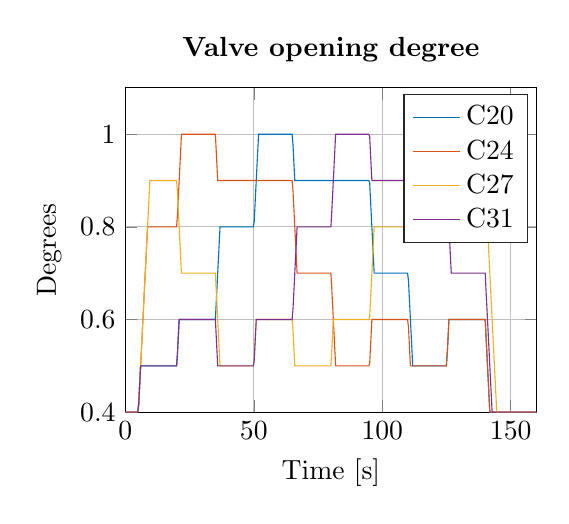
\begin{tikzpicture}

\begin{axis}[%
width=2.0556in,
height=1.62135in,
at={(1.011in,0.642in)},
scale only axis,
xmin=0,
xmax=160,
xlabel={Time [s]},
xmajorgrids,
ymin=0.4,
ymax=1.1,
ylabel={Degrees},
ymajorgrids,
axis background/.style={fill=white},
title style={font=\bfseries},
title={Valve opening degree},
legend style={legend cell align=left,align=left,draw=white!15!black}
]
\addplot [color=mycolor1,solid]
  table[row sep=crcr]{%
0	0.4\\
0.4	0.4\\
0.75	0.4\\
1.15	0.4\\
1.5	0.4\\
1.85	0.4\\
2.25	0.4\\
2.6	0.4\\
2.95	0.4\\
3.35	0.4\\
3.7	0.4\\
4.1	0.4\\
4.45	0.4\\
4.8	0.4\\
5.2	0.416666666666667\\
5.55	0.455555555555556\\
5.9	0.494444444444444\\
5.95	0.5\\
6.3	0.5\\
6.65	0.5\\
7.05	0.5\\
7.4	0.5\\
7.75	0.5\\
8.15	0.5\\
8.5	0.5\\
8.85	0.5\\
9.25	0.5\\
9.6	0.5\\
10	0.5\\
10.35	0.5\\
10.7	0.5\\
11.1	0.5\\
11.45	0.5\\
11.8	0.5\\
12.2	0.5\\
12.55	0.5\\
12.9	0.5\\
13.3	0.5\\
13.65	0.5\\
14.05	0.5\\
14.4	0.5\\
14.75	0.5\\
15.15	0.5\\
15.5	0.5\\
15.85	0.5\\
16.25	0.5\\
16.6	0.5\\
17	0.5\\
17.35	0.5\\
17.7	0.5\\
18.1	0.5\\
18.45	0.5\\
18.8	0.5\\
19.2	0.5\\
19.55	0.5\\
19.95	0.5\\
20.3	0.527777777777778\\
20.65	0.566666666666667\\
20.95	0.6\\
21.05	0.6\\
21.4	0.6\\
21.75	0.6\\
22.15	0.6\\
22.5	0.6\\
22.9	0.6\\
23.25	0.6\\
23.6	0.6\\
24	0.6\\
24.35	0.6\\
24.7	0.6\\
25.1	0.6\\
25.45	0.6\\
25.8	0.6\\
26.2	0.6\\
26.55	0.6\\
26.95	0.6\\
27.3	0.6\\
27.65	0.6\\
28.05	0.6\\
28.4	0.6\\
28.75	0.6\\
29.15	0.6\\
29.5	0.6\\
29.9	0.6\\
30.25	0.6\\
30.6	0.6\\
31	0.6\\
31.35	0.6\\
31.7	0.6\\
32.1	0.6\\
32.45	0.6\\
32.85	0.6\\
33.2	0.6\\
33.55	0.6\\
33.95	0.6\\
34.3	0.6\\
34.65	0.6\\
35.05	0.6\\
35.4	0.638888888888889\\
35.75	0.677777777777778\\
36.15	0.722222222222222\\
36.5	0.761111111111111\\
36.85	0.8\\
36.9	0.8\\
37.25	0.8\\
37.6	0.8\\
38	0.8\\
38.35	0.8\\
38.7	0.8\\
39.1	0.8\\
39.45	0.8\\
39.85	0.8\\
40.2	0.8\\
40.55	0.8\\
40.95	0.8\\
41.3	0.8\\
41.65	0.8\\
42.05	0.8\\
42.4	0.8\\
42.8	0.8\\
43.15	0.8\\
43.5	0.8\\
43.9	0.8\\
44.25	0.8\\
44.6	0.8\\
45	0.8\\
45.35	0.8\\
45.75	0.8\\
46.1	0.8\\
46.45	0.8\\
46.85	0.8\\
47.2	0.8\\
47.55	0.8\\
47.95	0.8\\
48.3	0.8\\
48.65	0.8\\
49.05	0.8\\
49.4	0.8\\
49.8	0.8\\
50.15	0.811111111111111\\
50.5	0.85\\
50.9	0.894444444444444\\
51.25	0.933333333333333\\
51.6	0.972222222222222\\
51.85	1\\
52	1\\
52.35	1\\
52.75	1\\
53.1	1\\
53.45	1\\
53.85	1\\
54.2	1\\
54.55	1\\
54.95	1\\
55.3	1\\
55.7	1\\
56.05	1\\
56.4	1\\
56.8	1\\
57.15	1\\
57.5	1\\
57.9	1\\
58.25	1\\
58.6	1\\
59	1\\
59.35	1\\
59.75	1\\
60.1	1\\
60.45	1\\
60.85	1\\
61.2	1\\
61.55	1\\
61.95	1\\
62.3	1\\
62.7	1\\
63.05	1\\
63.4	1\\
63.8	1\\
64.15	1\\
64.5	1\\
64.9	1\\
65.25	0.977777777777778\\
65.65	0.933333333333333\\
65.95	0.9\\
66	0.9\\
66.35	0.9\\
66.75	0.9\\
67.1	0.9\\
67.45	0.9\\
67.85	0.9\\
68.2	0.9\\
68.6	0.9\\
68.95	0.9\\
69.3	0.9\\
69.7	0.9\\
70.05	0.9\\
70.4	0.9\\
70.8	0.9\\
71.15	0.9\\
71.5	0.9\\
71.9	0.9\\
72.25	0.9\\
72.65	0.9\\
73	0.9\\
73.35	0.9\\
73.75	0.9\\
74.1	0.9\\
74.45	0.9\\
74.85	0.9\\
75.2	0.9\\
75.6	0.9\\
75.95	0.9\\
76.3	0.9\\
76.7	0.9\\
77.05	0.9\\
77.4	0.9\\
77.8	0.9\\
78.15	0.9\\
78.55	0.9\\
78.9	0.9\\
79.25	0.9\\
79.65	0.9\\
80	0.9\\
80.35	0.9\\
80.75	0.9\\
81.1	0.9\\
81.45	0.9\\
81.85	0.9\\
82.2	0.9\\
82.6	0.9\\
82.95	0.9\\
83.3	0.9\\
83.7	0.9\\
84.05	0.9\\
84.4	0.9\\
84.8	0.9\\
85.15	0.9\\
85.55	0.9\\
85.9	0.9\\
86.25	0.9\\
86.65	0.9\\
87	0.9\\
87.35	0.9\\
87.75	0.9\\
88.1	0.9\\
88.5	0.9\\
88.85	0.9\\
89.2	0.9\\
89.6	0.9\\
89.95	0.9\\
90.3	0.9\\
90.7	0.9\\
91.05	0.9\\
91.4	0.9\\
91.8	0.9\\
92.15	0.9\\
92.55	0.9\\
92.9	0.9\\
93.25	0.9\\
93.65	0.9\\
94	0.9\\
94.35	0.9\\
94.75	0.9\\
95.1	0.894444444444444\\
95.5	0.85\\
95.85	0.811111111111111\\
96.2	0.772222222222222\\
96.6	0.727777777777778\\
96.85	0.7\\
96.95	0.7\\
97.3	0.7\\
97.7	0.7\\
98.05	0.7\\
98.45	0.7\\
98.8	0.7\\
99.15	0.7\\
99.55	0.7\\
99.9	0.7\\
100.25	0.7\\
100.65	0.7\\
101	0.7\\
101.4	0.7\\
101.75	0.7\\
102.1	0.7\\
102.5	0.7\\
102.85	0.7\\
103.2	0.7\\
103.6	0.7\\
103.95	0.7\\
104.3	0.7\\
104.7	0.7\\
105.05	0.7\\
105.45	0.7\\
105.8	0.7\\
106.15	0.7\\
106.55	0.7\\
106.9	0.7\\
107.25	0.7\\
107.65	0.7\\
108	0.7\\
108.4	0.7\\
108.75	0.7\\
109.1	0.7\\
109.5	0.7\\
109.85	0.7\\
110.2	0.683333333333333\\
110.6	0.638888888888889\\
110.95	0.6\\
111.35	0.555555555555555\\
111.7	0.516666666666667\\
111.85	0.5\\
112.05	0.5\\
112.45	0.5\\
112.8	0.5\\
113.15	0.5\\
113.55	0.5\\
113.9	0.5\\
114.25	0.5\\
114.65	0.5\\
115	0.5\\
115.4	0.5\\
115.75	0.5\\
116.1	0.5\\
116.5	0.5\\
116.85	0.5\\
117.2	0.5\\
117.6	0.5\\
117.95	0.5\\
118.35	0.5\\
118.7	0.5\\
119.05	0.5\\
119.45	0.5\\
119.8	0.5\\
120.15	0.5\\
120.55	0.5\\
120.9	0.5\\
121.3	0.5\\
121.65	0.5\\
122	0.5\\
122.4	0.5\\
122.75	0.5\\
123.1	0.5\\
123.5	0.5\\
123.85	0.5\\
124.25	0.5\\
124.6	0.5\\
124.95	0.5\\
125.35	0.533333333333333\\
125.7	0.572222222222222\\
125.95	0.6\\
126.05	0.6\\
126.45	0.6\\
126.8	0.6\\
127.15	0.6\\
127.55	0.6\\
127.9	0.6\\
128.3	0.6\\
128.65	0.6\\
129	0.6\\
129.4	0.6\\
129.75	0.6\\
130.1	0.6\\
130.5	0.6\\
130.85	0.6\\
131.25	0.6\\
131.6	0.6\\
131.95	0.6\\
132.35	0.6\\
132.7	0.6\\
133.05	0.6\\
133.45	0.6\\
133.8	0.6\\
134.2	0.6\\
134.55	0.6\\
134.9	0.6\\
135.3	0.6\\
135.65	0.6\\
136	0.6\\
136.4	0.6\\
136.75	0.6\\
137.1	0.6\\
137.5	0.6\\
137.85	0.6\\
138.25	0.6\\
138.6	0.6\\
138.95	0.6\\
139.35	0.6\\
139.7	0.6\\
140.05	0.6\\
140.45	0.555555555555556\\
140.8	0.516666666666667\\
141.2	0.472222222222222\\
141.55	0.433333333333333\\
141.85	0.4\\
141.9	0.4\\
142.3	0.4\\
142.65	0.4\\
143	0.4\\
143.4	0.4\\
143.75	0.4\\
144.15	0.4\\
144.5	0.4\\
144.85	0.4\\
145.25	0.4\\
145.6	0.4\\
145.95	0.4\\
146.35	0.4\\
146.7	0.4\\
147.1	0.4\\
147.45	0.4\\
147.8	0.4\\
148.2	0.4\\
148.55	0.4\\
148.9	0.4\\
149.3	0.4\\
149.65	0.4\\
150	0.4\\
150.4	0.4\\
150.75	0.4\\
151.15	0.4\\
151.5	0.4\\
151.85	0.4\\
152.25	0.4\\
152.6	0.4\\
152.95	0.4\\
153.35	0.4\\
153.7	0.4\\
154.1	0.4\\
154.45	0.4\\
154.8	0.4\\
155.2	0.4\\
155.55	0.4\\
155.9	0.4\\
156.3	0.4\\
156.65	0.4\\
157.05	0.4\\
157.4	0.4\\
157.75	0.4\\
158.15	0.4\\
158.5	0.4\\
158.85	0.4\\
159.25	0.4\\
159.95	0.4\\
};
\addlegendentry{C20};

\addplot [color=mycolor2,solid]
  table[row sep=crcr]{%
0	0.4\\
0.4	0.4\\
0.75	0.4\\
1.15	0.4\\
1.5	0.4\\
1.85	0.4\\
2.25	0.4\\
2.6	0.4\\
2.95	0.4\\
3.35	0.4\\
3.7	0.4\\
4.1	0.4\\
4.45	0.4\\
4.8	0.4\\
5.2	0.416666666666667\\
5.55	0.455555555555556\\
5.9	0.494444444444444\\
6.3	0.538888888888889\\
6.65	0.577777777777778\\
7.05	0.622222222222222\\
7.4	0.661111111111111\\
7.75	0.7\\
8.15	0.744444444444444\\
8.5	0.783333333333333\\
8.65	0.8\\
8.85	0.8\\
9.25	0.8\\
9.6	0.8\\
10	0.8\\
10.35	0.8\\
10.7	0.8\\
11.1	0.8\\
11.45	0.8\\
11.8	0.8\\
12.2	0.8\\
12.55	0.8\\
12.9	0.8\\
13.3	0.8\\
13.65	0.8\\
14.05	0.8\\
14.4	0.8\\
14.75	0.8\\
15.15	0.8\\
15.5	0.8\\
15.85	0.8\\
16.25	0.8\\
16.6	0.8\\
17	0.8\\
17.35	0.8\\
17.7	0.8\\
18.1	0.8\\
18.45	0.8\\
18.8	0.8\\
19.2	0.8\\
19.55	0.8\\
19.95	0.8\\
20.3	0.827777777777778\\
20.65	0.866666666666667\\
21.05	0.911111111111111\\
21.4	0.95\\
21.75	0.988888888888889\\
21.85	1\\
22.15	1\\
22.5	1\\
22.9	1\\
23.25	1\\
23.6	1\\
24	1\\
24.35	1\\
24.7	1\\
25.1	1\\
25.45	1\\
25.8	1\\
26.2	1\\
26.55	1\\
26.95	1\\
27.3	1\\
27.65	1\\
28.05	1\\
28.4	1\\
28.75	1\\
29.15	1\\
29.5	1\\
29.9	1\\
30.25	1\\
30.6	1\\
31	1\\
31.35	1\\
31.7	1\\
32.1	1\\
32.45	1\\
32.85	1\\
33.2	1\\
33.55	1\\
33.95	1\\
34.3	1\\
34.65	1\\
35.05	1\\
35.4	0.961111111111111\\
35.75	0.922222222222222\\
35.95	0.9\\
36.15	0.9\\
36.5	0.9\\
36.9	0.9\\
37.25	0.9\\
37.6	0.9\\
38	0.9\\
38.35	0.9\\
38.7	0.9\\
39.1	0.9\\
39.45	0.9\\
39.85	0.9\\
40.2	0.9\\
40.55	0.9\\
40.95	0.9\\
41.3	0.9\\
41.65	0.9\\
42.05	0.9\\
42.4	0.9\\
42.8	0.9\\
43.15	0.9\\
43.5	0.9\\
43.9	0.9\\
44.25	0.9\\
44.6	0.9\\
45	0.9\\
45.35	0.9\\
45.75	0.9\\
46.1	0.9\\
46.45	0.9\\
46.85	0.9\\
47.2	0.9\\
47.55	0.9\\
47.95	0.9\\
48.3	0.9\\
48.65	0.9\\
49.05	0.9\\
49.4	0.9\\
49.8	0.9\\
50.15	0.9\\
50.5	0.9\\
50.9	0.9\\
51.25	0.9\\
51.6	0.9\\
52	0.9\\
52.35	0.9\\
52.75	0.9\\
53.1	0.9\\
53.45	0.9\\
53.85	0.9\\
54.2	0.9\\
54.55	0.9\\
54.95	0.9\\
55.3	0.9\\
55.7	0.9\\
56.05	0.9\\
56.4	0.9\\
56.8	0.9\\
57.15	0.9\\
57.5	0.9\\
57.9	0.9\\
58.25	0.9\\
58.6	0.9\\
59	0.9\\
59.35	0.9\\
59.75	0.9\\
60.1	0.9\\
60.45	0.9\\
60.85	0.9\\
61.2	0.9\\
61.55	0.9\\
61.95	0.9\\
62.3	0.9\\
62.7	0.9\\
63.05	0.9\\
63.4	0.9\\
63.8	0.9\\
64.15	0.9\\
64.5	0.9\\
64.9	0.9\\
65.25	0.877777777777778\\
65.65	0.833333333333333\\
66	0.794444444444445\\
66.35	0.755555555555556\\
66.75	0.711111111111111\\
66.85	0.7\\
67.1	0.7\\
67.45	0.7\\
67.85	0.7\\
68.2	0.7\\
68.6	0.7\\
68.95	0.7\\
69.3	0.7\\
69.7	0.7\\
70.05	0.7\\
70.4	0.7\\
70.8	0.7\\
71.15	0.7\\
71.5	0.7\\
71.9	0.7\\
72.25	0.7\\
72.65	0.7\\
73	0.7\\
73.35	0.7\\
73.75	0.7\\
74.1	0.7\\
74.45	0.7\\
74.85	0.7\\
75.2	0.7\\
75.6	0.7\\
75.95	0.7\\
76.3	0.7\\
76.7	0.7\\
77.05	0.7\\
77.4	0.7\\
77.8	0.7\\
78.15	0.7\\
78.55	0.7\\
78.9	0.7\\
79.25	0.7\\
79.65	0.7\\
80	0.7\\
80.35	0.666666666666667\\
80.75	0.622222222222222\\
81.1	0.583333333333333\\
81.45	0.544444444444444\\
81.85	0.5\\
81.9	0.5\\
82.2	0.5\\
82.6	0.5\\
82.95	0.5\\
83.3	0.5\\
83.7	0.5\\
84.05	0.5\\
84.4	0.5\\
84.8	0.5\\
85.15	0.5\\
85.55	0.5\\
85.9	0.5\\
86.25	0.5\\
86.65	0.5\\
87	0.5\\
87.35	0.5\\
87.75	0.5\\
88.1	0.5\\
88.5	0.5\\
88.85	0.5\\
89.2	0.5\\
89.6	0.5\\
89.95	0.5\\
90.3	0.5\\
90.7	0.5\\
91.05	0.5\\
91.4	0.5\\
91.8	0.5\\
92.15	0.5\\
92.55	0.5\\
92.9	0.5\\
93.25	0.5\\
93.65	0.5\\
94	0.5\\
94.35	0.5\\
94.75	0.5\\
95.1	0.505555555555556\\
95.5	0.55\\
95.85	0.588888888888889\\
95.95	0.6\\
96.2	0.6\\
96.6	0.6\\
96.95	0.6\\
97.3	0.6\\
97.7	0.6\\
98.05	0.6\\
98.45	0.6\\
98.8	0.6\\
99.15	0.6\\
99.55	0.6\\
99.9	0.6\\
100.25	0.6\\
100.65	0.6\\
101	0.6\\
101.4	0.6\\
101.75	0.6\\
102.1	0.6\\
102.5	0.6\\
102.85	0.6\\
103.2	0.6\\
103.6	0.6\\
103.95	0.6\\
104.3	0.6\\
104.7	0.6\\
105.05	0.6\\
105.45	0.6\\
105.8	0.6\\
106.15	0.6\\
106.55	0.6\\
106.9	0.6\\
107.25	0.6\\
107.65	0.6\\
108	0.6\\
108.4	0.6\\
108.75	0.6\\
109.1	0.6\\
109.5	0.6\\
109.85	0.6\\
110.2	0.583333333333333\\
110.6	0.538888888888889\\
110.95	0.5\\
111.35	0.5\\
111.7	0.5\\
112.05	0.5\\
112.45	0.5\\
112.8	0.5\\
113.15	0.5\\
113.55	0.5\\
113.9	0.5\\
114.25	0.5\\
114.65	0.5\\
115	0.5\\
115.4	0.5\\
115.75	0.5\\
116.1	0.5\\
116.5	0.5\\
116.85	0.5\\
117.2	0.5\\
117.6	0.5\\
117.95	0.5\\
118.35	0.5\\
118.7	0.5\\
119.05	0.5\\
119.45	0.5\\
119.8	0.5\\
120.15	0.5\\
120.55	0.5\\
120.9	0.5\\
121.3	0.5\\
121.65	0.5\\
122	0.5\\
122.4	0.5\\
122.75	0.5\\
123.1	0.5\\
123.5	0.5\\
123.85	0.5\\
124.25	0.5\\
124.6	0.5\\
124.95	0.5\\
125.35	0.533333333333333\\
125.7	0.572222222222222\\
125.95	0.6\\
126.05	0.6\\
126.45	0.6\\
126.8	0.6\\
127.15	0.6\\
127.55	0.6\\
127.9	0.6\\
128.3	0.6\\
128.65	0.6\\
129	0.6\\
129.4	0.6\\
129.75	0.6\\
130.1	0.6\\
130.5	0.6\\
130.85	0.6\\
131.25	0.6\\
131.6	0.6\\
131.95	0.6\\
132.35	0.6\\
132.7	0.6\\
133.05	0.6\\
133.45	0.6\\
133.8	0.6\\
134.2	0.6\\
134.55	0.6\\
134.9	0.6\\
135.3	0.6\\
135.65	0.6\\
136	0.6\\
136.4	0.6\\
136.75	0.6\\
137.1	0.6\\
137.5	0.6\\
137.85	0.6\\
138.25	0.6\\
138.6	0.6\\
138.95	0.6\\
139.35	0.6\\
139.7	0.6\\
140.05	0.6\\
140.45	0.555555555555556\\
140.8	0.516666666666667\\
141.2	0.472222222222222\\
141.55	0.433333333333333\\
141.85	0.4\\
141.9	0.4\\
142.3	0.4\\
142.65	0.4\\
143	0.4\\
143.4	0.4\\
143.75	0.4\\
144.15	0.4\\
144.5	0.4\\
144.85	0.4\\
145.25	0.4\\
145.6	0.4\\
145.95	0.4\\
146.35	0.4\\
146.7	0.4\\
147.1	0.4\\
147.45	0.4\\
147.8	0.4\\
148.2	0.4\\
148.55	0.4\\
148.9	0.4\\
149.3	0.4\\
149.65	0.4\\
150	0.4\\
150.4	0.4\\
150.75	0.4\\
151.15	0.4\\
151.5	0.4\\
151.85	0.4\\
152.25	0.4\\
152.6	0.4\\
152.95	0.4\\
153.35	0.4\\
153.7	0.4\\
154.1	0.4\\
154.45	0.4\\
154.8	0.4\\
155.2	0.4\\
155.55	0.4\\
155.9	0.4\\
156.3	0.4\\
156.65	0.4\\
157.05	0.4\\
157.4	0.4\\
157.75	0.4\\
158.15	0.4\\
158.5	0.4\\
158.85	0.4\\
159.25	0.4\\
159.95	0.4\\
};
\addlegendentry{C24};

\addplot [color=mycolor3,solid]
  table[row sep=crcr]{%
0	0.4\\
0.4	0.4\\
0.75	0.4\\
1.15	0.4\\
1.5	0.4\\
1.85	0.4\\
2.25	0.4\\
2.6	0.4\\
2.95	0.4\\
3.35	0.4\\
3.7	0.4\\
4.1	0.4\\
4.45	0.4\\
4.8	0.4\\
5.2	0.416666666666667\\
5.55	0.455555555555556\\
5.9	0.494444444444444\\
6.3	0.538888888888889\\
6.65	0.577777777777778\\
7.05	0.622222222222222\\
7.4	0.661111111111111\\
7.75	0.7\\
8.15	0.744444444444444\\
8.5	0.783333333333333\\
8.85	0.822222222222222\\
9.25	0.866666666666667\\
9.55	0.9\\
9.6	0.9\\
10	0.9\\
10.35	0.9\\
10.7	0.9\\
11.1	0.9\\
11.45	0.9\\
11.8	0.9\\
12.2	0.9\\
12.55	0.9\\
12.9	0.9\\
13.3	0.9\\
13.65	0.9\\
14.05	0.9\\
14.4	0.9\\
14.75	0.9\\
15.15	0.9\\
15.5	0.9\\
15.85	0.9\\
16.25	0.9\\
16.6	0.9\\
17	0.9\\
17.35	0.9\\
17.7	0.9\\
18.1	0.9\\
18.45	0.9\\
18.8	0.9\\
19.2	0.9\\
19.55	0.9\\
19.95	0.9\\
20.3	0.872222222222222\\
20.65	0.833333333333333\\
21.05	0.788888888888889\\
21.4	0.75\\
21.75	0.711111111111111\\
21.85	0.7\\
22.15	0.7\\
22.5	0.7\\
22.9	0.7\\
23.25	0.7\\
23.6	0.7\\
24	0.7\\
24.35	0.7\\
24.7	0.7\\
25.1	0.7\\
25.45	0.7\\
25.8	0.7\\
26.2	0.7\\
26.55	0.7\\
26.95	0.7\\
27.3	0.7\\
27.65	0.7\\
28.05	0.7\\
28.4	0.7\\
28.75	0.7\\
29.15	0.7\\
29.5	0.7\\
29.9	0.7\\
30.25	0.7\\
30.6	0.7\\
31	0.7\\
31.35	0.7\\
31.7	0.7\\
32.1	0.7\\
32.45	0.7\\
32.85	0.7\\
33.2	0.7\\
33.55	0.7\\
33.95	0.7\\
34.3	0.7\\
34.65	0.7\\
35.05	0.7\\
35.4	0.661111111111111\\
35.75	0.622222222222222\\
36.15	0.577777777777778\\
36.5	0.538888888888889\\
36.85	0.5\\
36.9	0.5\\
37.25	0.5\\
37.6	0.5\\
38	0.5\\
38.35	0.5\\
38.7	0.5\\
39.1	0.5\\
39.45	0.5\\
39.85	0.5\\
40.2	0.5\\
40.55	0.5\\
40.95	0.5\\
41.3	0.5\\
41.65	0.5\\
42.05	0.5\\
42.4	0.5\\
42.8	0.5\\
43.15	0.5\\
43.5	0.5\\
43.9	0.5\\
44.25	0.5\\
44.6	0.5\\
45	0.5\\
45.35	0.5\\
45.75	0.5\\
46.1	0.5\\
46.45	0.5\\
46.85	0.5\\
47.2	0.5\\
47.55	0.5\\
47.95	0.5\\
48.3	0.5\\
48.65	0.5\\
49.05	0.5\\
49.4	0.5\\
49.8	0.5\\
50.15	0.511111111111111\\
50.5	0.55\\
50.9	0.594444444444444\\
50.95	0.6\\
51.25	0.6\\
51.6	0.6\\
52	0.6\\
52.35	0.6\\
52.75	0.6\\
53.1	0.6\\
53.45	0.6\\
53.85	0.6\\
54.2	0.6\\
54.55	0.6\\
54.95	0.6\\
55.3	0.6\\
55.7	0.6\\
56.05	0.6\\
56.4	0.6\\
56.8	0.6\\
57.15	0.6\\
57.5	0.6\\
57.9	0.6\\
58.25	0.6\\
58.6	0.6\\
59	0.6\\
59.35	0.6\\
59.75	0.6\\
60.1	0.6\\
60.45	0.6\\
60.85	0.6\\
61.2	0.6\\
61.55	0.6\\
61.95	0.6\\
62.3	0.6\\
62.7	0.6\\
63.05	0.6\\
63.4	0.6\\
63.8	0.6\\
64.15	0.6\\
64.5	0.6\\
64.9	0.6\\
65.25	0.577777777777778\\
65.65	0.533333333333333\\
65.95	0.5\\
66	0.5\\
66.35	0.5\\
66.75	0.5\\
67.1	0.5\\
67.45	0.5\\
67.85	0.5\\
68.2	0.5\\
68.6	0.5\\
68.95	0.5\\
69.3	0.5\\
69.7	0.5\\
70.05	0.5\\
70.4	0.5\\
70.8	0.5\\
71.15	0.5\\
71.5	0.5\\
71.9	0.5\\
72.25	0.5\\
72.65	0.5\\
73	0.5\\
73.35	0.5\\
73.75	0.5\\
74.1	0.5\\
74.45	0.5\\
74.85	0.5\\
75.2	0.5\\
75.6	0.5\\
75.95	0.5\\
76.3	0.5\\
76.7	0.5\\
77.05	0.5\\
77.4	0.5\\
77.8	0.5\\
78.15	0.5\\
78.55	0.5\\
78.9	0.5\\
79.25	0.5\\
79.65	0.5\\
80	0.5\\
80.35	0.533333333333333\\
80.75	0.577777777777778\\
80.95	0.6\\
81.1	0.6\\
81.45	0.6\\
81.85	0.6\\
82.2	0.6\\
82.6	0.6\\
82.95	0.6\\
83.3	0.6\\
83.7	0.6\\
84.05	0.6\\
84.4	0.6\\
84.8	0.6\\
85.15	0.6\\
85.55	0.6\\
85.9	0.6\\
86.25	0.6\\
86.65	0.6\\
87	0.6\\
87.35	0.6\\
87.75	0.6\\
88.1	0.6\\
88.5	0.6\\
88.85	0.6\\
89.2	0.6\\
89.6	0.6\\
89.95	0.6\\
90.3	0.6\\
90.7	0.6\\
91.05	0.6\\
91.4	0.6\\
91.8	0.6\\
92.15	0.6\\
92.55	0.6\\
92.9	0.6\\
93.25	0.6\\
93.65	0.6\\
94	0.6\\
94.35	0.6\\
94.75	0.6\\
95.1	0.605555555555556\\
95.5	0.65\\
95.85	0.688888888888889\\
96.2	0.727777777777778\\
96.6	0.772222222222222\\
96.85	0.8\\
96.95	0.8\\
97.3	0.8\\
97.7	0.8\\
98.05	0.8\\
98.45	0.8\\
98.8	0.8\\
99.15	0.8\\
99.55	0.8\\
99.9	0.8\\
100.25	0.8\\
100.65	0.8\\
101	0.8\\
101.4	0.8\\
101.75	0.8\\
102.1	0.8\\
102.5	0.8\\
102.85	0.8\\
103.2	0.8\\
103.6	0.8\\
103.95	0.8\\
104.3	0.8\\
104.7	0.8\\
105.05	0.8\\
105.45	0.8\\
105.8	0.8\\
106.15	0.8\\
106.55	0.8\\
106.9	0.8\\
107.25	0.8\\
107.65	0.8\\
108	0.8\\
108.4	0.8\\
108.75	0.8\\
109.1	0.8\\
109.5	0.8\\
109.85	0.8\\
110.2	0.816666666666667\\
110.6	0.861111111111111\\
110.95	0.9\\
111.35	0.944444444444445\\
111.7	0.983333333333333\\
111.85	1\\
112.05	1\\
112.45	1\\
112.8	1\\
113.15	1\\
113.55	1\\
113.9	1\\
114.25	1\\
114.65	1\\
115	1\\
115.4	1\\
115.75	1\\
116.1	1\\
116.5	1\\
116.85	1\\
117.2	1\\
117.6	1\\
117.95	1\\
118.35	1\\
118.7	1\\
119.05	1\\
119.45	1\\
119.8	1\\
120.15	1\\
120.55	1\\
120.9	1\\
121.3	1\\
121.65	1\\
122	1\\
122.4	1\\
122.75	1\\
123.1	1\\
123.5	1\\
123.85	1\\
124.25	1\\
124.6	1\\
124.95	1\\
125.35	0.966666666666667\\
125.7	0.927777777777778\\
125.95	0.9\\
126.05	0.9\\
126.45	0.9\\
126.8	0.9\\
127.15	0.9\\
127.55	0.9\\
127.9	0.9\\
128.3	0.9\\
128.65	0.9\\
129	0.9\\
129.4	0.9\\
129.75	0.9\\
130.1	0.9\\
130.5	0.9\\
130.85	0.9\\
131.25	0.9\\
131.6	0.9\\
131.95	0.9\\
132.35	0.9\\
132.7	0.9\\
133.05	0.9\\
133.45	0.9\\
133.8	0.9\\
134.2	0.9\\
134.55	0.9\\
134.9	0.9\\
135.3	0.9\\
135.65	0.9\\
136	0.9\\
136.4	0.9\\
136.75	0.9\\
137.1	0.9\\
137.5	0.9\\
137.85	0.9\\
138.25	0.9\\
138.6	0.9\\
138.95	0.9\\
139.35	0.9\\
139.7	0.9\\
140.05	0.9\\
140.45	0.855555555555556\\
140.8	0.816666666666667\\
141.2	0.772222222222222\\
141.55	0.733333333333333\\
141.9	0.694444444444444\\
142.3	0.65\\
142.65	0.611111111111111\\
143	0.572222222222222\\
143.4	0.527777777777778\\
143.75	0.488888888888889\\
144.15	0.444444444444444\\
144.5	0.405555555555556\\
144.55	0.4\\
144.85	0.4\\
145.25	0.4\\
145.6	0.4\\
145.95	0.4\\
146.35	0.4\\
146.7	0.4\\
147.1	0.4\\
147.45	0.4\\
147.8	0.4\\
148.2	0.4\\
148.55	0.4\\
148.9	0.4\\
149.3	0.4\\
149.65	0.4\\
150	0.4\\
150.4	0.4\\
150.75	0.4\\
151.15	0.4\\
151.5	0.4\\
151.85	0.4\\
152.25	0.4\\
152.6	0.4\\
152.95	0.4\\
153.35	0.4\\
153.7	0.4\\
154.1	0.4\\
154.45	0.4\\
154.8	0.4\\
155.2	0.4\\
155.55	0.4\\
155.9	0.4\\
156.3	0.4\\
156.65	0.4\\
157.05	0.4\\
157.4	0.4\\
157.75	0.4\\
158.15	0.4\\
158.5	0.4\\
158.85	0.4\\
159.25	0.4\\
159.95	0.4\\
};
\addlegendentry{C27};

\addplot [color=mycolor4,solid]
  table[row sep=crcr]{%
0	0.4\\
0.4	0.4\\
0.75	0.4\\
1.15	0.4\\
1.5	0.4\\
1.85	0.4\\
2.25	0.4\\
2.6	0.4\\
2.95	0.4\\
3.35	0.4\\
3.7	0.4\\
4.1	0.4\\
4.45	0.4\\
4.8	0.4\\
5.2	0.416666666666667\\
5.55	0.455555555555556\\
5.9	0.494444444444444\\
5.95	0.5\\
6.3	0.5\\
6.65	0.5\\
7.05	0.5\\
7.4	0.5\\
7.75	0.5\\
8.15	0.5\\
8.5	0.5\\
8.85	0.5\\
9.25	0.5\\
9.6	0.5\\
10	0.5\\
10.35	0.5\\
10.7	0.5\\
11.1	0.5\\
11.45	0.5\\
11.8	0.5\\
12.2	0.5\\
12.55	0.5\\
12.9	0.5\\
13.3	0.5\\
13.65	0.5\\
14.05	0.5\\
14.4	0.5\\
14.75	0.5\\
15.15	0.5\\
15.5	0.5\\
15.85	0.5\\
16.25	0.5\\
16.6	0.5\\
17	0.5\\
17.35	0.5\\
17.7	0.5\\
18.1	0.5\\
18.45	0.5\\
18.8	0.5\\
19.2	0.5\\
19.55	0.5\\
19.95	0.5\\
20.3	0.527777777777778\\
20.65	0.566666666666667\\
20.95	0.6\\
21.05	0.6\\
21.4	0.6\\
21.75	0.6\\
22.15	0.6\\
22.5	0.6\\
22.9	0.6\\
23.25	0.6\\
23.6	0.6\\
24	0.6\\
24.35	0.6\\
24.7	0.6\\
25.1	0.6\\
25.45	0.6\\
25.8	0.6\\
26.2	0.6\\
26.55	0.6\\
26.95	0.6\\
27.3	0.6\\
27.65	0.6\\
28.05	0.6\\
28.4	0.6\\
28.75	0.6\\
29.15	0.6\\
29.5	0.6\\
29.9	0.6\\
30.25	0.6\\
30.6	0.6\\
31	0.6\\
31.35	0.6\\
31.7	0.6\\
32.1	0.6\\
32.45	0.6\\
32.85	0.6\\
33.2	0.6\\
33.55	0.6\\
33.95	0.6\\
34.3	0.6\\
34.65	0.6\\
35.05	0.6\\
35.4	0.561111111111111\\
35.75	0.522222222222222\\
35.95	0.5\\
36.15	0.5\\
36.5	0.5\\
36.9	0.5\\
37.25	0.5\\
37.6	0.5\\
38	0.5\\
38.35	0.5\\
38.7	0.5\\
39.1	0.5\\
39.45	0.5\\
39.85	0.5\\
40.2	0.5\\
40.55	0.5\\
40.95	0.5\\
41.3	0.5\\
41.65	0.5\\
42.05	0.5\\
42.4	0.5\\
42.8	0.5\\
43.15	0.5\\
43.5	0.5\\
43.9	0.5\\
44.25	0.5\\
44.6	0.5\\
45	0.5\\
45.35	0.5\\
45.75	0.5\\
46.1	0.5\\
46.45	0.5\\
46.85	0.5\\
47.2	0.5\\
47.55	0.5\\
47.95	0.5\\
48.3	0.5\\
48.65	0.5\\
49.05	0.5\\
49.4	0.5\\
49.8	0.5\\
50.15	0.511111111111111\\
50.5	0.55\\
50.9	0.594444444444444\\
50.95	0.6\\
51.25	0.6\\
51.6	0.6\\
52	0.6\\
52.35	0.6\\
52.75	0.6\\
53.1	0.6\\
53.45	0.6\\
53.85	0.6\\
54.2	0.6\\
54.55	0.6\\
54.95	0.6\\
55.3	0.6\\
55.7	0.6\\
56.05	0.6\\
56.4	0.6\\
56.8	0.6\\
57.15	0.6\\
57.5	0.6\\
57.9	0.6\\
58.25	0.6\\
58.6	0.6\\
59	0.6\\
59.35	0.6\\
59.75	0.6\\
60.1	0.6\\
60.45	0.6\\
60.85	0.6\\
61.2	0.6\\
61.55	0.6\\
61.95	0.6\\
62.3	0.6\\
62.7	0.6\\
63.05	0.6\\
63.4	0.6\\
63.8	0.6\\
64.15	0.6\\
64.5	0.6\\
64.9	0.6\\
65.25	0.622222222222222\\
65.65	0.666666666666667\\
66	0.705555555555555\\
66.35	0.744444444444444\\
66.75	0.788888888888889\\
66.85	0.8\\
67.1	0.8\\
67.45	0.8\\
67.85	0.8\\
68.2	0.8\\
68.6	0.8\\
68.95	0.8\\
69.3	0.8\\
69.7	0.8\\
70.05	0.8\\
70.4	0.8\\
70.8	0.8\\
71.15	0.8\\
71.5	0.8\\
71.9	0.8\\
72.25	0.8\\
72.65	0.8\\
73	0.8\\
73.35	0.8\\
73.75	0.8\\
74.1	0.8\\
74.45	0.8\\
74.85	0.8\\
75.2	0.8\\
75.6	0.8\\
75.95	0.8\\
76.3	0.8\\
76.7	0.8\\
77.05	0.8\\
77.4	0.8\\
77.8	0.8\\
78.15	0.8\\
78.55	0.8\\
78.9	0.8\\
79.25	0.8\\
79.65	0.8\\
80	0.8\\
80.35	0.833333333333333\\
80.75	0.877777777777778\\
81.1	0.916666666666667\\
81.45	0.955555555555556\\
81.85	1\\
82.2	1\\
82.6	1\\
82.95	1\\
83.3	1\\
83.7	1\\
84.05	1\\
84.4	1\\
84.8	1\\
85.15	1\\
85.55	1\\
85.9	1\\
86.25	1\\
86.65	1\\
87	1\\
87.35	1\\
87.75	1\\
88.1	1\\
88.5	1\\
88.85	1\\
89.2	1\\
89.6	1\\
89.95	1\\
90.3	1\\
90.7	1\\
91.05	1\\
91.4	1\\
91.8	1\\
92.15	1\\
92.55	1\\
92.9	1\\
93.25	1\\
93.65	1\\
94	1\\
94.35	1\\
94.75	1\\
95.1	0.994444444444444\\
95.5	0.95\\
95.85	0.911111111111111\\
95.95	0.9\\
96.2	0.9\\
96.6	0.9\\
96.95	0.9\\
97.3	0.9\\
97.7	0.9\\
98.05	0.9\\
98.45	0.9\\
98.8	0.9\\
99.15	0.9\\
99.55	0.9\\
99.9	0.9\\
100.25	0.9\\
100.65	0.9\\
101	0.9\\
101.4	0.9\\
101.75	0.9\\
102.1	0.9\\
102.5	0.9\\
102.85	0.9\\
103.2	0.9\\
103.6	0.9\\
103.95	0.9\\
104.3	0.9\\
104.7	0.9\\
105.05	0.9\\
105.45	0.9\\
105.8	0.9\\
106.15	0.9\\
106.55	0.9\\
106.9	0.9\\
107.25	0.9\\
107.65	0.9\\
108	0.9\\
108.4	0.9\\
108.75	0.9\\
109.1	0.9\\
109.5	0.9\\
109.85	0.9\\
110.2	0.9\\
110.6	0.9\\
110.95	0.9\\
111.35	0.9\\
111.7	0.9\\
112.05	0.9\\
112.45	0.9\\
112.8	0.9\\
113.15	0.9\\
113.55	0.9\\
113.9	0.9\\
114.25	0.9\\
114.65	0.9\\
115	0.9\\
115.4	0.9\\
115.75	0.9\\
116.1	0.9\\
116.5	0.9\\
116.85	0.9\\
117.2	0.9\\
117.6	0.9\\
117.95	0.9\\
118.35	0.9\\
118.7	0.9\\
119.05	0.9\\
119.45	0.9\\
119.8	0.9\\
120.15	0.9\\
120.55	0.9\\
120.9	0.9\\
121.3	0.9\\
121.65	0.9\\
122	0.9\\
122.4	0.9\\
122.75	0.9\\
123.1	0.9\\
123.5	0.9\\
123.85	0.9\\
124.25	0.9\\
124.6	0.9\\
124.95	0.9\\
125.35	0.866666666666667\\
125.7	0.827777777777778\\
126.05	0.788888888888889\\
126.45	0.744444444444444\\
126.8	0.705555555555556\\
126.85	0.7\\
127.15	0.7\\
127.55	0.7\\
127.9	0.7\\
128.3	0.7\\
128.65	0.7\\
129	0.7\\
129.4	0.7\\
129.75	0.7\\
130.1	0.7\\
130.5	0.7\\
130.85	0.7\\
131.25	0.7\\
131.6	0.7\\
131.95	0.7\\
132.35	0.7\\
132.7	0.7\\
133.05	0.7\\
133.45	0.7\\
133.8	0.7\\
134.2	0.7\\
134.55	0.7\\
134.9	0.7\\
135.3	0.7\\
135.65	0.7\\
136	0.7\\
136.4	0.7\\
136.75	0.7\\
137.1	0.7\\
137.5	0.7\\
137.85	0.7\\
138.25	0.7\\
138.6	0.7\\
138.95	0.7\\
139.35	0.7\\
139.7	0.7\\
140.05	0.7\\
140.45	0.655555555555556\\
140.8	0.616666666666667\\
141.2	0.572222222222222\\
141.55	0.533333333333333\\
141.9	0.494444444444444\\
142.3	0.45\\
142.65	0.411111111111111\\
142.75	0.4\\
143	0.4\\
143.4	0.4\\
143.75	0.4\\
144.15	0.4\\
144.5	0.4\\
144.85	0.4\\
145.25	0.4\\
145.6	0.4\\
145.95	0.4\\
146.35	0.4\\
146.7	0.4\\
147.1	0.4\\
147.45	0.4\\
147.8	0.4\\
148.2	0.4\\
148.55	0.4\\
148.9	0.4\\
149.3	0.4\\
149.65	0.4\\
150	0.4\\
150.4	0.4\\
150.75	0.4\\
151.15	0.4\\
151.5	0.4\\
151.85	0.4\\
152.25	0.4\\
152.6	0.4\\
152.95	0.4\\
153.35	0.4\\
153.7	0.4\\
154.1	0.4\\
154.45	0.4\\
154.8	0.4\\
155.2	0.4\\
155.55	0.4\\
155.9	0.4\\
156.3	0.4\\
156.65	0.4\\
157.05	0.4\\
157.4	0.4\\
157.75	0.4\\
158.15	0.4\\
158.5	0.4\\
158.85	0.4\\
159.25	0.4\\
159.95	0.4\\
};
\addlegendentry{C31};

\end{axis}
\end{tikzpicture}% 
    \caption{Inputs to the parameter identification}
  \end{minipage}
  \hfill
  \begin{minipage}[b]{0.45\textwidth}
    % This file was created by matlab2tikz.
%
%The latest updates can be retrieved from
%  http://www.mathworks.com/matlabcentral/fileexchange/22022-matlab2tikz-matlab2tikz
%where you can also make suggestions and rate matlab2tikz.
%
\definecolor{mycolor1}{rgb}{0.00000,0.44700,0.74100}%
\definecolor{mycolor2}{rgb}{0.85000,0.32500,0.09800}%
%
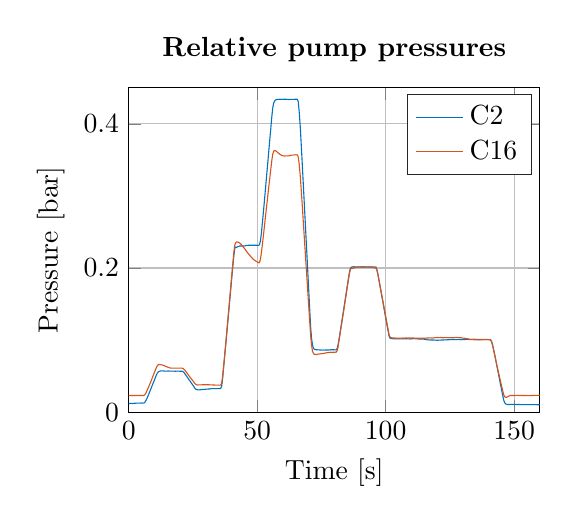
\begin{tikzpicture}

\begin{axis}[%
width=2.0556in,
height=1.62135in,
at={(1.011in,0.642in)},
scale only axis,
xmin=0,
xmax=160,
xlabel={Time [s]},
xmajorgrids,
ymin=0,
ymax=0.45,
ylabel={Pressure [bar]},
ymajorgrids,
axis background/.style={fill=white},
title style={font=\bfseries},
title={Relative pump pressures},
legend style={legend cell align=left,align=left,draw=white!15!black}
]
\addplot [color=mycolor1,solid]
  table[row sep=crcr]{%
0	0.0119562561094821\\
0.15	0.0119379276637343\\
0.35	0.0119990224828936\\
0.4	0.0119990224828936\\
0.75	0.0120967741935485\\
0.85	0.0121639784946238\\
1.15	0.012145650048876\\
1.5	0.012047898338221\\
1.65	0.0119929130009777\\
1.85	0.0120234604105573\\
2.25	0.0122556207233628\\
2.5	0.0123594819159337\\
2.6	0.0123106060606062\\
2.95	0.0124266862170089\\
3.2	0.0124877810361683\\
3.5	0.0124511241446727\\
3.65	0.0125061094819161\\
3.7	0.0125061094819161\\
3.8	0.0124877810361683\\
4.2	0.0125427663734117\\
4.4	0.0124755620723364\\
4.45	0.0124816715542524\\
4.8	0.01269550342131\\
5.2	0.0125855327468232\\
5.5	0.0125183284457479\\
5.55	0.0125244379276638\\
5.9	0.0126099706744869\\
6.3	0.0137829912023461\\
6.65	0.0158663245356794\\
7.05	0.0187194525904204\\
7.4	0.0213770772238515\\
7.75	0.0244440371456501\\
8.15	0.0279630987292278\\
8.5	0.0311766862170088\\
8.85	0.0343658357771261\\
9.25	0.0379093352883676\\
9.6	0.0409824046920822\\
10	0.0445320136852396\\
10.35	0.0476600684261975\\
10.7	0.0508369990224829\\
11.1	0.0539711632453568\\
11.45	0.055608504398827\\
11.8	0.0565371456500489\\
12.2	0.0570136852394917\\
12.55	0.0572030791788856\\
12.85	0.0572519550342131\\
12.9	0.0572458455522971\\
13.3	0.0571542033235581\\
13.65	0.057074780058651\\
13.8	0.0570992179863147\\
14.05	0.0569525904203323\\
14.4	0.056891495601173\\
14.45	0.0568548387096773\\
14.75	0.0569159335288367\\
15.15	0.0570564516129031\\
15.2	0.0570442326490713\\
15.4	0.0570992179863147\\
15.5	0.0570808895405669\\
15.75	0.0569892473118279\\
15.9	0.0570014662756598\\
16.2	0.0569220430107526\\
16.3	0.0569342619745845\\
16.5	0.0568670576735093\\
16.6	0.0568792766373412\\
16.9	0.0568487292277615\\
17.15	0.0568365102639296\\
17.35	0.056897605083089\\
17.45	0.0569220430107528\\
17.7	0.0568792766373414\\
17.95	0.0566898826979474\\
18.1	0.0567021016617793\\
18.45	0.0568059628543502\\
18.75	0.0568731671554256\\
18.85	0.0568609481915937\\
19.1	0.0569037145650054\\
19.25	0.0568853861192576\\
19.5	0.056952590420333\\
19.55	0.0569464809384171\\
19.9	0.056763196480939\\
19.95	0.056763196480939\\
20.2	0.0566715542522002\\
20.3	0.056683773216032\\
20.65	0.0567509775171074\\
20.8	0.0567631964809393\\
21.05	0.0564943792766382\\
21.4	0.0554252199413497\\
21.75	0.0538550830889548\\
22.15	0.0518389540566966\\
22.5	0.0499450146627571\\
22.9	0.0480144183773219\\
23.25	0.046157135874878\\
23.6	0.0443487292277615\\
24	0.0423448191593352\\
24.35	0.0405364125122187\\
24.7	0.0388379765395889\\
25.1	0.0367485337243395\\
25.45	0.0348912512218955\\
25.8	0.0330584066471153\\
26.2	0.0316776637341142\\
26.55	0.0312072336265873\\
26.95	0.0310117302052774\\
27.3	0.0309323069403703\\
27.45	0.0308895405669588\\
27.6	0.0309445259042023\\
27.65	0.0309261974584545\\
28.05	0.0311950146627556\\
28.4	0.0313660801564017\\
28.6	0.0313477517106539\\
28.75	0.0314760508308885\\
28.9	0.0314393939393928\\
29.15	0.0315554740957955\\
29.25	0.0315676930596274\\
29.45	0.0315371456500477\\
29.5	0.0315493646138796\\
29.9	0.0317326490713576\\
30.25	0.0318731671554242\\
30.55	0.0319586999022473\\
30.6	0.0319586999022473\\
30.9	0.0320686705767341\\
31.05	0.0320381231671544\\
31.15	0.0320747800586501\\
31.35	0.0320564516129023\\
31.7	0.0322947214076237\\
32	0.0324718963831859\\
32.1	0.0324718963831859\\
32.4	0.0327040566959913\\
32.55	0.0326673998044957\\
32.85	0.0327284946236551\\
33.1	0.0326429618768318\\
33.2	0.0326429618768318\\
33.5	0.0325940860215044\\
33.65	0.0326490713587478\\
33.8	0.0325879765395883\\
33.95	0.032624633431084\\
34.05	0.0326001955034202\\
34.35	0.0325940860215042\\
34.55	0.0326429618768318\\
34.9	0.0326185239491679\\
35.05	0.0325635386119244\\
35.4	0.0326551808406634\\
35.75	0.0328262463343096\\
36.15	0.0355388563049842\\
36.5	0.0448619257086988\\
36.9	0.060929863147604\\
37.25	0.0741691104594321\\
37.6	0.0875549853372427\\
38	0.102840909090908\\
38.35	0.11649560117302\\
38.7	0.130419110459432\\
39.1	0.146395405669599\\
39.45	0.160355571847507\\
39.85	0.176240224828935\\
40.2	0.190108748778104\\
40.55	0.203714565004889\\
40.95	0.21831622678397\\
41.3	0.227663734115348\\
41.55	0.228885630498535\\
41.75	0.228366324535681\\
42.05	0.228897849462367\\
42.4	0.229521016617793\\
42.8	0.22999144672532\\
43.15	0.230504643206259\\
43.5	0.230620723362661\\
43.9	0.230498533724343\\
44	0.230529081133922\\
44.35	0.230486314760511\\
44.6	0.230571847507334\\
45	0.230632942326493\\
45.35	0.230730694037148\\
45.75	0.231341642228742\\
45.85	0.23146383186706\\
46.1	0.231372189638321\\
46.45	0.23152492668622\\
46.85	0.231634897360706\\
47.2	0.231555474095799\\
47.25	0.231561583577715\\
47.5	0.23152492668622\\
47.55	0.231537145650051\\
47.9	0.231714320625613\\
47.95	0.231695992179866\\
48.3	0.231537145650051\\
48.35	0.231531036168136\\
48.65	0.231586021505379\\
48.9	0.23165933528837\\
49.1	0.231641006842622\\
49.2	0.231665444770286\\
49.4	0.231653225806454\\
49.8	0.231531036168136\\
49.95	0.23149437927664\\
50.35	0.231512707722388\\
50.5	0.231476050830892\\
50.9	0.232355816226786\\
51.25	0.237396138807431\\
51.6	0.247391251221898\\
52	0.261638563049856\\
52.35	0.275146627565985\\
52.75	0.29068914956012\\
53.1	0.30493035190616\\
53.45	0.319061583577714\\
53.85	0.335215053763442\\
54.2	0.349327956989248\\
54.55	0.363599706744868\\
54.95	0.379905913978494\\
55.3	0.393939393939393\\
55.7	0.41005009775171\\
56.05	0.422134652981426\\
56.4	0.428763440860213\\
56.8	0.431885386119255\\
57.15	0.433082844574777\\
57.5	0.433773216031277\\
57.8	0.434029814271746\\
57.95	0.434005376344084\\
58.25	0.434121456500488\\
58.5	0.434145894428154\\
58.6	0.434121456500491\\
59	0.434176441837736\\
59.25	0.434097018572831\\
59.45	0.434139784946244\\
59.65	0.433987047898347\\
59.75	0.434035923753675\\
60.1	0.434176441837744\\
60.4	0.434280303030317\\
60.55	0.434243646138822\\
60.8	0.434304740957984\\
60.85	0.434286412512236\\
61.05	0.434133675464339\\
61.2	0.434188660801584\\
61.55	0.434084799609015\\
61.75	0.434084799609016\\
61.95	0.433956500488783\\
62.1	0.433925953079205\\
62.3	0.433932062561122\\
62.7	0.434017595307948\\
62.75	0.434023704789864\\
63.05	0.433956500488789\\
63.15	0.433919843597293\\
63.4	0.433956500488789\\
63.8	0.434005376344116\\
63.9	0.434072580645192\\
64.15	0.434042033235613\\
64.5	0.43409090909094\\
64.7	0.434261974584586\\
65	0.434213098729259\\
65.2	0.434237536656922\\
65.25	0.434231427175006\\
65.65	0.433974828934536\\
66	0.430321358748804\\
66.35	0.416654447702858\\
66.75	0.396627565982426\\
67.1	0.374272971652023\\
67.45	0.350635386119273\\
67.85	0.323197702834812\\
68.2	0.298869745845562\\
68.6	0.270986070381238\\
68.95	0.246700879765399\\
69.3	0.222330156402738\\
69.7	0.194312072336264\\
70.05	0.170032991202341\\
70.4	0.145747800586502\\
70.8	0.118334555229708\\
71.15	0.102657624633424\\
71.5	0.0935300586510177\\
71.9	0.0883797653958855\\
72.25	0.0873228250244296\\
72.65	0.086772971651996\\
73	0.0865957966764341\\
73.35	0.0865163734115271\\
73.55	0.0864491691104519\\
73.75	0.0864491691104519\\
74.1	0.0863453079178811\\
74.3	0.08627199413489\\
74.45	0.0863208699902174\\
74.85	0.0861620234604032\\
75.2	0.0860826001954962\\
75.45	0.0860764907135803\\
75.6	0.0861131476050758\\
75.85	0.0861681329423192\\
75.95	0.0861436950146555\\
76.25	0.0860887096774121\\
76.3	0.0861131476050758\\
76.7	0.0862475562072262\\
76.9	0.0862231182795625\\
77.05	0.0862781036168059\\
77.1	0.0862842130987218\\
77.2	0.0862536656891422\\
77.55	0.0863025415444696\\
77.8	0.0862108993157307\\
77.9	0.086186461388067\\
78.15	0.0863330889540492\\
78.55	0.0865408113391908\\
78.7	0.0865530303030226\\
78.85	0.0865347018572749\\
78.9	0.0865408113391908\\
79.25	0.0866263440860138\\
79.3	0.0866324535679297\\
79.65	0.0865347018572749\\
79.8	0.0865530303030226\\
80	0.0864858260019474\\
80.15	0.0864247311827882\\
80.35	0.08643695014662\\
80.7	0.0864858260019474\\
80.75	0.0864858260019474\\
81.1	0.0881598240469128\\
81.45	0.0927724828934434\\
81.85	0.101454056695987\\
82.2	0.108993157380252\\
82.6	0.118047409579668\\
82.95	0.126209677419358\\
83.3	0.134133675464327\\
83.7	0.143212365591407\\
84.05	0.151337976539601\\
84.4	0.159543010752702\\
84.8	0.168908846529831\\
85.15	0.177126099706764\\
85.55	0.18627199413492\\
85.9	0.193976050830915\\
86.25	0.199382942326518\\
86.6	0.201038611925738\\
86.65	0.201038611925738\\
87	0.201423509286442\\
87.35	0.201686217008827\\
87.6	0.201747311827987\\
87.75	0.201625122189668\\
87.9	0.201551808406677\\
88.1	0.201570136852425\\
88.5	0.201661779081164\\
88.85	0.201582355816257\\
88.9	0.201588465298173\\
89.2	0.201496823069434\\
89.45	0.201527370479013\\
89.7	0.201539589442845\\
89.85	0.201454056696022\\
90.1	0.201423509286442\\
90.25	0.201466275659854\\
90.4	0.201478494623686\\
90.5	0.20144183773219\\
90.7	0.201466275659854\\
91	0.201386852394947\\
91.05	0.201399071358779\\
91.4	0.201350195503451\\
91.65	0.201380742913031\\
91.8	0.201331867057704\\
92.15	0.20130742913004\\
92.4	0.201325757575788\\
92.55	0.201270772238544\\
92.6	0.201252443792796\\
92.9	0.201295210166208\\
93.15	0.201356304985367\\
93.4	0.201319648093872\\
93.6	0.201374633431115\\
93.85	0.201417399804527\\
94	0.201344086021535\\
94.1	0.201331867057704\\
94.3	0.201405180840695\\
94.35	0.201392961876863\\
94.6	0.201484604105602\\
94.75	0.201454056696022\\
94.85	0.201392961876863\\
95.1	0.201411290322611\\
95.25	0.201460166177938\\
95.5	0.201447947214106\\
95.85	0.201063049853402\\
96	0.200647605083117\\
96.2	0.201454056696019\\
96.6	0.197519550342155\\
96.95	0.191666666666691\\
97.3	0.184927908113418\\
97.7	0.177040566959949\\
98.05	0.170216275659853\\
98.45	0.162286168132972\\
98.8	0.155278592375398\\
99.15	0.148319892473151\\
99.55	0.140298142717532\\
99.9	0.133339442815285\\
100.25	0.12625855327472\\
100.65	0.118310117302092\\
101	0.112017350928684\\
101.4	0.104508797654006\\
101.75	0.102669843597312\\
102.1	0.102046676441887\\
102.5	0.101942815249316\\
102.55	0.101955034213148\\
102.85	0.101863391984409\\
103.2	0.101741202346091\\
103.45	0.101722873900343\\
103.7	0.101735092864175\\
103.95	0.101838954056745\\
104.1	0.101857282502493\\
104.3	0.101747311828007\\
104.5	0.101728983382259\\
104.7	0.101790078201418\\
104.75	0.101808406647166\\
104.85	0.101783968719502\\
105.05	0.101796187683334\\
105.45	0.101722873900343\\
105.7	0.101735092864175\\
105.8	0.101698435972679\\
105.95	0.101667888563099\\
106.25	0.101649560117352\\
106.45	0.101765640273754\\
106.55	0.101722873900343\\
106.85	0.101619012707772\\
106.9	0.101631231671604\\
107.05	0.101765640273754\\
107.25	0.101747311828007\\
107.65	0.101814516129082\\
107.85	0.101851173020577\\
108	0.101820625610998\\
108.35	0.101753421309922\\
108.45	0.101765640273754\\
108.75	0.101661779081184\\
109.1	0.101625122189688\\
109.5	0.101533479960949\\
109.85	0.101588465298192\\
110.2	0.101759530791838\\
110.5	0.101930596285484\\
110.6	0.101906158357821\\
110.85	0.101955034213148\\
110.95	0.1019367057674\\
111.2	0.101979472140812\\
111.35	0.101979472140812\\
111.7	0.101857282502493\\
111.85	0.101863391984409\\
112.05	0.101698435972679\\
112.25	0.101722873900343\\
112.45	0.101667888563099\\
112.8	0.101515151515201\\
113.15	0.101454056696042\\
113.45	0.101392961876883\\
113.55	0.101392961876883\\
113.9	0.101435728250294\\
114.15	0.101454056696042\\
114.25	0.101411290322631\\
114.35	0.101423509286462\\
114.65	0.101368523949219\\
115	0.101197458455573\\
115.35	0.100867546432113\\
115.4	0.100873655914029\\
115.75	0.100714809384215\\
116.1	0.100562072336317\\
116.5	0.100274926686268\\
116.55	0.100281036168184\\
116.85	0.100177174975613\\
116.9	0.100158846529865\\
117.15	0.100207722385193\\
117.2	0.100195503421361\\
117.6	0.10012218963837\\
117.7	0.100152737047949\\
118.15	0.100164956011781\\
118.35	0.100036656891547\\
118.45	0.100006109481967\\
118.65	0.100073313783042\\
118.7	0.100073313783042\\
119.05	0.09992668621706\\
119.35	0.0998594819159848\\
119.45	0.0998717008798167\\
119.8	0.0998167155425733\\
120.1	0.0996639784946751\\
120.15	0.099670087976591\\
120.55	0.0998350439883211\\
120.6	0.0998594819159848\\
121	0.0998350439883211\\
121.3	0.0999633431085556\\
121.65	0.100103861192622\\
121.85	0.100201612903277\\
122	0.100183284457529\\
122.35	0.100085532746874\\
122.4	0.10009164222879\\
122.75	0.100219941349025\\
122.85	0.100250488758604\\
123.2	0.100213831867109\\
123.4	0.100384897360755\\
123.55	0.100354349951175\\
123.65	0.100378787878839\\
123.85	0.100366568915007\\
124.25	0.10045210166183\\
124.5	0.100500977517157\\
124.6	0.100494868035241\\
124.95	0.100592619745896\\
125.35	0.100635386119308\\
125.5	0.100623167155476\\
125.7	0.100684261974635\\
126	0.100788123167206\\
126.1	0.100794232649122\\
126.45	0.100580400782064\\
126.65	0.100555962854401\\
126.75	0.100592619745896\\
126.8	0.100592619745896\\
126.9	0.10061705767356\\
127.3	0.100659824046971\\
127.45	0.100604838709728\\
127.55	0.10061705767356\\
127.65	0.100598729227812\\
127.9	0.10061705767356\\
128.2	0.100678152492719\\
128.3	0.100665933528887\\
128.65	0.100537634408653\\
128.9	0.100604838709728\\
129	0.100568181818232\\
129.2	0.100507086999073\\
129.4	0.100525415444821\\
129.6	0.100555962854401\\
129.75	0.100549853372485\\
130.1	0.100727028348047\\
130.45	0.100861436950197\\
130.5	0.100861436950197\\
130.85	0.100794232649122\\
131.25	0.100983626588516\\
131.45	0.101130254154498\\
131.6	0.101050830889591\\
131.95	0.100928641251272\\
132.3	0.100836999022533\\
132.35	0.100861436950197\\
132.5	0.100983626588516\\
132.7	0.100873655914029\\
132.9	0.100843108504449\\
133.05	0.100855327468281\\
133.45	0.100989736070431\\
133.65	0.10108137829917\\
133.9	0.100995845552347\\
134.15	0.101105816226834\\
134.2	0.101105816226834\\
134.35	0.101044721407675\\
134.55	0.101063049853423\\
134.7	0.101093597263002\\
134.9	0.101069159335339\\
135.3	0.100971407624684\\
135.4	0.100965298142768\\
135.65	0.101032502443843\\
135.95	0.100940860215104\\
136	0.100940860215104\\
136.4	0.100739247311878\\
136.7	0.100885874877861\\
136.75	0.100885874877861\\
136.95	0.100934750733188\\
137.3	0.100971407624684\\
137.5	0.100818670576786\\
137.55	0.100794232649122\\
137.75	0.100849217986365\\
137.85	0.10081256109487\\
138	0.100745356793794\\
138.25	0.100775904203374\\
138.55	0.100702590420383\\
138.6	0.100714809384215\\
138.9	0.100861436950197\\
139	0.100843108504449\\
139.35	0.100891984359777\\
139.4	0.100898093841693\\
139.7	0.100806451612954\\
140.05	0.100672043010803\\
140.45	0.100568181818232\\
140.65	0.10058651026398\\
140.8	0.100384897360755\\
141.2	0.0982282502444242\\
141.55	0.0940493646139196\\
141.9	0.0885508308895744\\
142.3	0.0817143206256397\\
142.65	0.0757209188661044\\
143	0.0694525904203523\\
143.4	0.0621945259042185\\
143.75	0.0556573802541656\\
144.15	0.0483993157380318\\
144.5	0.0420821114369524\\
144.85	0.0358260019550322\\
145.25	0.0287512218963762\\
145.6	0.0223790322580534\\
145.95	0.0165933528836604\\
146.35	0.0128299120234487\\
146.7	0.0114552785923649\\
147.1	0.0108260019550244\\
147.45	0.0106182795698828\\
147.5	0.0106243890517987\\
147.7	0.0105694037145554\\
147.8	0.010599951124135\\
148.15	0.0106671554252102\\
148.3	0.0106121700879669\\
148.55	0.0107160312805377\\
148.85	0.0107771260996969\\
148.95	0.0107649071358651\\
149.2	0.0108015640273607\\
149.3	0.010771016617781\\
149.65	0.0108015640273607\\
149.7	0.0108076735092766\\
149.95	0.0107160312805377\\
150.1	0.0107404692082014\\
150.3	0.010685483870958\\
150.5	0.0107343597262854\\
150.7	0.0106488269794625\\
150.75	0.0106549364613784\\
151.1	0.0105877321603032\\
151.15	0.0105938416422191\\
151.35	0.0106488269794625\\
151.55	0.0106366080156306\\
151.75	0.0105632942326395\\
151.85	0.0105694037145554\\
152	0.0105083088953961\\
152.25	0.0105266373411439\\
152.55	0.0104655425219846\\
152.65	0.0105083088953961\\
152.9	0.0104655425219846\\
153	0.0105021994134802\\
153.15	0.0104716520039005\\
153.35	0.0104777614858165\\
153.5	0.0104227761485731\\
153.7	0.0104594330400687\\
153.85	0.0103983382209094\\
154.15	0.0103983382209094\\
154.3	0.0104594330400687\\
154.6	0.010434995112405\\
154.7	0.0103922287389935\\
154.8	0.010434995112405\\
154.95	0.010514418377312\\
155.35	0.0104411045943209\\
155.55	0.0104655425219846\\
155.7	0.010428885630489\\
155.9	0.0104838709677324\\
156	0.0104716520039005\\
156.15	0.0105327468230598\\
156.3	0.0104716520039005\\
156.6	0.0104166666666572\\
156.65	0.0104227761485731\\
157	0.0104838709677324\\
157.05	0.0104777614858165\\
157.25	0.0104227761485731\\
157.4	0.010428885630489\\
157.6	0.0103800097751616\\
157.75	0.0103922287389935\\
158.15	0.0103555718474979\\
158.2	0.010349462365582\\
158.35	0.0104044477028253\\
158.55	0.0103800097751616\\
158.85	0.0103311339198342\\
159.25	0.0102394916910953\\
159.45	0.0102761485825908\\
159.6	0.0102150537634316\\
159.95	0.010263929618759\\
};
\addlegendentry{C2};

\addplot [color=mycolor2,solid]
  table[row sep=crcr]{%
0	0.0229472140762463\\
0.2	0.022886119257087\\
0.4	0.0229227761485826\\
0.75	0.0230021994134897\\
1	0.0230571847507331\\
1.25	0.0230144183773216\\
1.5	0.0230816226783968\\
1.75	0.023069403714565\\
1.85	0.0231182795698925\\
2.15	0.0230510752688172\\
2.25	0.023069403714565\\
2.3	0.0230938416422287\\
2.6	0.0230755131964809\\
2.95	0.0231304985337244\\
3.35	0.0231915933528837\\
3.65	0.023258797653959\\
3.7	0.023258797653959\\
4.05	0.0231366080156403\\
4.2	0.0231182795698925\\
4.45	0.023161045943304\\
4.65	0.0230938416422287\\
4.9	0.0231671554252199\\
5.05	0.0231060606060606\\
5.2	0.0231427174975562\\
5.55	0.0230510752688171\\
5.6	0.0230449657869012\\
5.9	0.0231671554252198\\
6.3	0.02424853372434\\
6.65	0.0262646627565981\\
7.05	0.0292216520039099\\
7.4	0.0320686705767349\\
7.75	0.0349584555229714\\
8.15	0.0383797653958941\\
8.5	0.0414222873900292\\
8.85	0.0445442326490712\\
9.25	0.0482710166177907\\
9.6	0.0514540566959919\\
10	0.0550769794721405\\
10.35	0.0582783479960897\\
10.7	0.0613453079178884\\
11.1	0.0642961876832845\\
11.45	0.0656830400782014\\
11.8	0.0661412512218964\\
12.2	0.065988514173998\\
12.55	0.0658113391984358\\
12.9	0.0655730694037142\\
13.3	0.065133186705767\\
13.65	0.0647177419354834\\
14.05	0.064094574780058\\
14.4	0.0635691593352876\\
14.75	0.063074291300097\\
15.15	0.0624816715542513\\
15.5	0.0619134897360695\\
15.85	0.061565249266861\\
16.25	0.0611864613880729\\
16.6	0.0609909579667629\\
16.65	0.060978739002931\\
16.85	0.0610276148582584\\
17.05	0.0610031769305947\\
17.15	0.0610276148582584\\
17.35	0.0610031769305947\\
17.7	0.0610642717497541\\
17.9	0.0611070381231657\\
18.1	0.0610459433040063\\
18.45	0.0611070381231656\\
18.5	0.0611131476050815\\
18.6	0.0611009286412497\\
19	0.0611131476050815\\
19.2	0.0610642717497541\\
19.45	0.0609848484848469\\
19.6	0.0610459433040062\\
19.8	0.0609970674486787\\
20.1	0.0609848484848468\\
20.3	0.061064271749754\\
20.45	0.061058162267838\\
20.6	0.0611253665689133\\
20.65	0.0611131476050814\\
21.05	0.0607710166177893\\
21.4	0.0598423753665675\\
21.75	0.0586326979472128\\
22.15	0.0567876344086011\\
22.5	0.0551014173998038\\
22.9	0.0531280547409574\\
23.25	0.0513685239491688\\
23.6	0.0497372922776147\\
24	0.0478372434017596\\
24.35	0.0462487781036171\\
24.7	0.0446603128054746\\
25.1	0.0428824535679381\\
25.45	0.0412084555229725\\
25.8	0.0396016617790822\\
26.2	0.0383980938416432\\
26.55	0.0378665689149571\\
26.75	0.037701612903227\\
26.95	0.0377260508308907\\
27.25	0.0377688172043022\\
27.3	0.0377627077223862\\
27.55	0.0378421309872933\\
27.65	0.0378238025415455\\
28.05	0.0379276637341163\\
28.4	0.0379032258064526\\
28.5	0.0378910068426207\\
28.75	0.0379765395894437\\
29.1	0.0380987292277624\\
29.15	0.0380987292277624\\
29.2	0.0380681818181827\\
29.5	0.0380865102639305\\
29.75	0.0380254154447712\\
30.15	0.0380070869990234\\
30.25	0.0380315249266872\\
30.4	0.0379887585532757\\
30.65	0.0380193059628553\\
30.75	0.0379826490713597\\
31	0.0379887585532757\\
31.25	0.0379215542522005\\
31.4	0.0379459921798642\\
31.65	0.0378543499511252\\
31.8	0.0379093352883686\\
32.05	0.0378115835777137\\
32.1	0.0378115835777137\\
32.45	0.0377382697947226\\
32.5	0.0377443792766385\\
32.8	0.0375855327468244\\
32.85	0.0375916422287403\\
33	0.0376344086021518\\
33.35	0.0376344086021518\\
33.55	0.0375794232649085\\
33.75	0.0375244379276651\\
33.95	0.0375305474095811\\
34.1	0.0375000000000014\\
34.4	0.0375061094819173\\
34.5	0.0375427663734129\\
34.7	0.0375305474095811\\
34.95	0.0374633431085059\\
35.05	0.0375000000000014\\
35.25	0.0375488758553288\\
35.65	0.0375000000000014\\
35.75	0.0375672043010766\\
36.15	0.0396810850439893\\
36.5	0.0480205278592387\\
36.9	0.0617790811339214\\
37.25	0.0750610948191607\\
37.6	0.0888074291300111\\
38	0.104881476050832\\
38.35	0.118884408602151\\
38.7	0.132985092864125\\
39.1	0.149120234604105\\
39.45	0.163257575757575\\
39.85	0.179368279569892\\
40.2	0.193413978494622\\
40.55	0.20740469208211\\
40.95	0.222947214076245\\
41.3	0.232019794721406\\
41.65	0.234915689149558\\
42.05	0.236149804496577\\
42.15	0.236204789833821\\
42.4	0.236021505376343\\
42.8	0.235612170087976\\
43.15	0.234640762463343\\
43.5	0.233760997067448\\
43.9	0.232227517106549\\
44.25	0.230712365591399\\
44.6	0.229032258064518\\
45	0.227339931573805\\
45.35	0.225733137829915\\
45.75	0.223662023460413\\
46.1	0.221963587487782\\
46.45	0.220259042033236\\
46.85	0.218566715542521\\
47.2	0.217106549364612\\
47.55	0.215609726295207\\
47.95	0.21410068426197\\
48.3	0.212689393939388\\
48.65	0.211644672531763\\
49.05	0.210575513196474\\
49.4	0.209781280547401\\
49.8	0.20889540566959\\
50.15	0.208174486803508\\
50.5	0.20756964809383\\
50.65	0.207319159335277\\
50.9	0.207642961876823\\
51.25	0.21203567937438\\
51.6	0.220155180840657\\
52	0.231805962854343\\
52.35	0.242882453567931\\
52.75	0.255694037145645\\
53.1	0.267149315738021\\
53.45	0.278445747800582\\
53.85	0.291477272727269\\
54.2	0.302840909090905\\
54.55	0.313892961876828\\
54.95	0.326460166177904\\
55.3	0.337255620723358\\
55.7	0.349480694037141\\
56.05	0.357887341153466\\
56.4	0.36201124144672\\
56.8	0.363098729227755\\
56.85	0.363159824046915\\
57.15	0.362646627565976\\
57.5	0.362072336265879\\
57.9	0.360532746823063\\
58.25	0.359494134897356\\
58.6	0.358644916911045\\
59	0.357380254154449\\
59.35	0.356763196480942\\
59.75	0.356103372434024\\
60.1	0.355614613880752\\
60.3	0.355675708699913\\
60.45	0.355608504398838\\
60.75	0.355382453567949\\
60.85	0.355504643206268\\
61	0.355694037145663\\
61.35	0.355571847507347\\
61.45	0.355541300097767\\
61.7	0.355657380254171\\
61.85	0.355522971652022\\
61.95	0.355559628543518\\
62.3	0.355724584555251\\
62.7	0.355962854349975\\
63.05	0.35640884652984\\
63.4	0.356695992179888\\
63.65	0.356604349951149\\
63.8	0.356683773216056\\
63.9	0.356732649071384\\
64.15	0.356732649071384\\
64.45	0.357025904203351\\
64.7	0.357019794721434\\
64.9	0.356952590420358\\
65.1	0.357245845552322\\
65.25	0.357062561094843\\
65.35	0.356946480938441\\
65.65	0.357044232649096\\
66	0.353885630498555\\
66.35	0.344312072336286\\
66.75	0.328512952101683\\
67.1	0.310703812316734\\
67.45	0.291947702834815\\
67.85	0.26971529814273\\
68.2	0.249993890518095\\
68.6	0.227718719452599\\
68.95	0.20846774193549\\
69.3	0.188966275659828\\
69.7	0.16681329423265\\
70.05	0.147403470185729\\
70.4	0.128164711632453\\
70.8	0.106286656891495\\
71.15	0.093407869012708\\
71.5	0.0847690615835759\\
71.9	0.0813660801563998\\
72.25	0.0802908113391965\\
72.55	0.079905913978493\\
72.65	0.079905913978493\\
73	0.0800097751710638\\
73.35	0.0802113880742894\\
73.75	0.0805046432062539\\
74.1	0.0807001466275636\\
74.45	0.0807978983382185\\
74.5	0.0807856793743866\\
74.85	0.0810483870967715\\
75.2	0.0812377810361653\\
75.35	0.0812194525904175\\
75.6	0.0813782991202316\\
75.95	0.0815676930596254\\
76.3	0.0818365102639262\\
76.7	0.0820931085043952\\
77.05	0.0823863636363598\\
77.1	0.0823802541544438\\
77.4	0.082532991202342\\
77.8	0.0827162756598199\\
78.15	0.0829484359726251\\
78.55	0.0830889540566915\\
78.65	0.0830950635386074\\
78.9	0.0829545454545411\\
79.15	0.0829239980449614\\
79.25	0.0829912023460366\\
79.6	0.083125610948187\\
79.65	0.0831195014662711\\
79.75	0.0830645161290278\\
80	0.0831133919843552\\
80.35	0.0831622678396826\\
80.65	0.0832294721407578\\
80.75	0.0832050342130941\\
81.1	0.0850195503421258\\
81.45	0.0898582600195457\\
81.85	0.0993279569892451\\
82.2	0.107233626588463\\
82.6	0.116410068426197\\
82.95	0.124346285434996\\
83.3	0.13250244379277\\
83.7	0.141752199413496\\
84.05	0.149841153470194\\
84.4	0.15794843597264\\
84.8	0.167271505376358\\
85.15	0.175543743890534\\
85.55	0.184799608993176\\
85.9	0.192436461388096\\
86.25	0.197880009775195\\
86.5	0.199456256109507\\
86.65	0.199291300097777\\
87	0.199389051808433\\
87.35	0.199835043988298\\
87.75	0.200268817204331\\
88.1	0.200507086999053\\
88.5	0.200775904203353\\
88.85	0.201056940371487\\
89.2	0.201325757575788\\
89.5	0.201368523949199\\
89.65	0.201356304985367\\
89.95	0.201197458455553\\
90.3	0.20147238514177\\
90.5	0.201619012707752\\
90.7	0.201588465298173\\
90.85	0.201728983382239\\
91.1	0.201570136852425\\
91.4	0.20166788856308\\
91.5	0.201722873900323\\
91.75	0.201527370479013\\
91.8	0.201527370479013\\
92	0.201698435972659\\
92.15	0.201692326490743\\
92.45	0.201521260997097\\
92.75	0.201655669599248\\
92.9	0.201551808406677\\
93.2	0.20144183773219\\
93.25	0.201447947214106\\
93.65	0.201179130009805\\
94	0.201014173998075\\
94.15	0.201087487781066\\
94.35	0.200946969696999\\
94.5	0.200934750733168\\
94.75	0.201020283479991\\
94.8	0.201026392961906\\
95.1	0.200861436950176\\
95.45	0.200647605083119\\
95.5	0.200647605083119\\
95.85	0.20020772238517\\
95.9	0.200109970674515\\
96.15	0.200610948191621\\
96.2	0.200568181818209\\
96.6	0.197244623655938\\
96.95	0.191813294232672\\
97.3	0.185282258064535\\
97.7	0.177419354838725\\
98.05	0.170815004887596\\
98.45	0.162872678396879\\
98.8	0.156231671554255\\
99.15	0.149370723362658\\
99.55	0.141721652003906\\
99.9	0.134811827956981\\
100.25	0.12812194525903\\
100.65	0.120387341153454\\
101	0.113697458455506\\
101.4	0.106304985337225\\
101.75	0.104184995112393\\
102.1	0.103250244379254\\
102.5	0.103018084066449\\
102.7	0.103054740957944\\
102.85	0.102908113391962\\
102.95	0.102847018572803\\
103.5	0.102956989247289\\
103.6	0.102871456500466\\
103.95	0.102706500488737\\
104.3	0.102578201368507\\
104.7	0.102633186705756\\
104.75	0.102633186705757\\
105	0.102565982404685\\
105.2	0.102510997067445\\
105.45	0.102578201368524\\
105.6	0.10260263929619\\
105.75	0.102535434995117\\
105.8	0.102535434995117\\
106.15	0.102682062561104\\
106.55	0.102798142717513\\
106.7	0.102853128054758\\
106.9	0.102767595307938\\
107.05	0.102816471163268\\
107.2	0.102737047898363\\
107.25	0.102737047898363\\
107.65	0.10287145650052\\
107.7	0.102865347018604\\
107.95	0.102938660801599\\
108	0.102914222873936\\
108.4	0.102773704789875\\
108.5	0.102761485826045\\
108.75	0.102956989247358\\
108.8	0.102993646138854\\
109	0.102950879765444\\
109.15	0.102975317693108\\
109.5	0.102920332355865\\
109.7	0.10282258064521\\
109.85	0.102883675464369\\
109.95	0.102950879765444\\
110.2	0.102932551319697\\
110.6	0.102834799609042\\
110.85	0.102840909090958\\
110.95	0.102785923753714\\
111.3	0.102547653958993\\
111.4	0.102584310850489\\
111.7	0.102486559139834\\
111.75	0.102474340176002\\
112.05	0.102523216031329\\
112.2	0.102596529814321\\
112.45	0.102584310850489\\
112.65	0.102480449657918\\
112.8	0.102529325513245\\
113.15	0.102633186705816\\
113.2	0.102663734115396\\
113.55	0.102639296187732\\
113.8	0.102498778103666\\
113.9	0.102504887585582\\
114.25	0.102468230694086\\
114.35	0.102443792766422\\
114.65	0.102523216031329\\
114.75	0.102584310850489\\
115	0.102504887585582\\
115.35	0.102584310850489\\
115.4	0.102578201368573\\
115.75	0.102743157380303\\
116.1	0.102938660801613\\
116.3	0.103005865102688\\
116.45	0.102889784946285\\
116.65	0.102895894428201\\
116.85	0.102932551319697\\
117.2	0.103042521994183\\
117.5	0.102993646138856\\
117.65	0.103048631476099\\
117.95	0.102902003910117\\
118.15	0.102816471163294\\
118.35	0.102914222873949\\
118.7	0.103024193548436\\
119.05	0.103207478005913\\
119.4	0.103354105571896\\
119.45	0.103354105571896\\
119.8	0.103457966764466\\
120	0.103549608993205\\
120.25	0.103519061583626\\
120.55	0.103464076246382\\
120.7	0.103506842619794\\
120.85	0.103439638318719\\
120.9	0.10345185728255\\
121.2	0.10351295210171\\
121.5	0.103488514174046\\
121.65	0.103549608993205\\
122	0.103384652981475\\
122.25	0.103231915933577\\
122.45	0.103280791788904\\
122.75	0.103354105571896\\
122.95	0.103427419354887\\
123.1	0.103421309872971\\
123.4	0.103506842619794\\
123.55	0.103464076246382\\
123.85	0.103537390029373\\
124.25	0.103335777126148\\
124.4	0.103311339198484\\
124.6	0.1033174486804\\
124.75	0.103280791788904\\
124.95	0.103299120234652\\
125.2	0.103366324535727\\
125.55	0.103360215053812\\
125.7	0.10328690127082\\
125.8	0.103225806451661\\
126.1	0.103231915933577\\
126.45	0.10334799608998\\
126.6	0.103299120234652\\
126.8	0.103360215053812\\
127.15	0.103622922776196\\
127.45	0.103696236559188\\
127.55	0.103635141740028\\
127.9	0.103555718475121\\
128.05	0.103629032258112\\
128.3	0.10345185728255\\
128.65	0.10334799608998\\
129	0.103164711632502\\
129.25	0.103231915933577\\
129.4	0.103170821114418\\
129.75	0.102963098729276\\
130.1	0.102694281524975\\
130.5	0.102535434995161\\
130.85	0.102510997067498\\
131.25	0.102181085044037\\
131.6	0.102040566959971\\
131.95	0.101790078201418\\
132.35	0.101392961876883\\
132.7	0.101099706744918\\
133.05	0.100910312805524\\
133.45	0.100794232649122\\
133.8	0.100629276637392\\
134	0.100672043010803\\
134.2	0.100555962854401\\
134.55	0.100482649071409\\
134.75	0.100397116324586\\
135	0.100354349951175\\
135.2	0.100445992179914\\
135.3	0.100384897360755\\
135.65	0.100305474095848\\
136	0.100329912023511\\
136.1	0.100311583577763\\
136.3	0.100372678396923\\
136.4	0.100372678396923\\
136.55	0.100439882697998\\
136.75	0.100378787878839\\
136.95	0.100415444770334\\
137.2	0.100488758553325\\
137.4	0.100391006842671\\
137.5	0.100403225806502\\
137.85	0.100568181818232\\
137.95	0.100543743890569\\
138.25	0.100568181818232\\
138.45	0.100690371456551\\
138.65	0.100690371456551\\
138.95	0.100568181818232\\
139.2	0.100574291300148\\
139.35	0.100525415444821\\
139.6	0.100635386119308\\
139.75	0.10064760508314\\
140.05	0.100537634408653\\
140.4	0.100439882697998\\
140.45	0.100445992179914\\
140.8	0.100219941349025\\
141.2	0.0978739002933018\\
141.55	0.0936827956989653\\
141.9	0.0884836265885006\\
142.3	0.0819342619746145\\
142.65	0.0759958455523226\\
143	0.0697214076246546\\
143.4	0.062952101661795\\
143.75	0.0574108015640384\\
144.15	0.0512463343108557\\
144.5	0.045796676441838\\
144.85	0.0404447702834752\\
145.25	0.0343291788856199\\
145.6	0.0289283968719296\\
145.95	0.024065249266841\\
146.35	0.0213037634408408\\
146.7	0.0205767350928454\\
147.05	0.0207416911045755\\
147.1	0.0207294721407436\\
147.45	0.0211937927663541\\
147.8	0.0219147116324336\\
148.2	0.0227272727272521\\
148.55	0.0229533235581414\\
148.9	0.0231366080156192\\
149.05	0.0230999511241237\\
149.35	0.0231304985337033\\
149.6	0.023069403714544\\
149.65	0.02307551319646\\
149.8	0.0231488269794511\\
150.15	0.0231182795698714\\
150.4	0.0232099217986104\\
150.65	0.0232832355816015\\
150.85	0.0232710166177696\\
150.95	0.0233015640273493\\
151.15	0.0232710166177696\\
151.5	0.0233015640273493\\
151.85	0.0231427174975352\\
151.9	0.0231121700879555\\
152.25	0.0232160312805263\\
152.3	0.0232343597262741\\
152.6	0.0231304985337033\\
152.95	0.0230510752687962\\
153.3	0.0230877321602918\\
153.35	0.0230816226783759\\
153.5	0.0231243890517874\\
153.8	0.0231182795698714\\
154.1	0.0230571847507122\\
154.15	0.0230388563049644\\
154.4	0.023069403714544\\
154.45	0.023069403714544\\
154.8	0.0229960899315529\\
155.05	0.0229411045943095\\
155.2	0.0229716520038892\\
155.4	0.022904447702814\\
155.6	0.0229105571847299\\
155.85	0.0229594330400573\\
155.9	0.0229594330400573\\
156.3	0.022989980449637\\
156.45	0.022983870967721\\
156.65	0.0230388563049644\\
156.95	0.0230938416422077\\
157.3	0.02307551319646\\
157.4	0.0231121700879555\\
157.7	0.0232038123166944\\
157.8	0.0231915933528626\\
158	0.02324046920819\\
158.15	0.02324046920819\\
158.5	0.0231732649071148\\
158.7	0.0232465786901059\\
158.85	0.0232221407624422\\
159.2	0.0233015640273493\\
159.25	0.0233015640273493\\
159.55	0.0233748778103404\\
159.95	0.023411534701836\\
};
\addlegendentry{C16};

\end{axis}
\end{tikzpicture}% 
    \caption{Output pressure measurements}
  \end{minipage}
  \label{fig:nonlinearpumps}
\end{figure}

%The estimation process, based on the applied input data, tries to fit the established output signal data to the simulation output. In the physical setup $8$ 
%different pressure relative sensors are available which are used as output signals. \figref{systemdiagram1} shows the pressure measurements in the different 
%nodes.


Together with the inputs from the lab and the nonlinear differential model the nonlinear parameter estimation is carried out. 

\begin{figure}[H]
  \centering
  \begin{minipage}[b]{0.45\textwidth}
    % This file was created by matlab2tikz.
%
%The latest updates can be retrieved from
%  http://www.mathworks.com/matlabcentral/fileexchange/22022-matlab2tikz-matlab2tikz
%where you can also make suggestions and rate matlab2tikz.
%
\definecolor{mycolor1}{rgb}{0.00000,0.44700,0.74100}%
\definecolor{mycolor2}{rgb}{0.85000,0.32500,0.09800}%
%
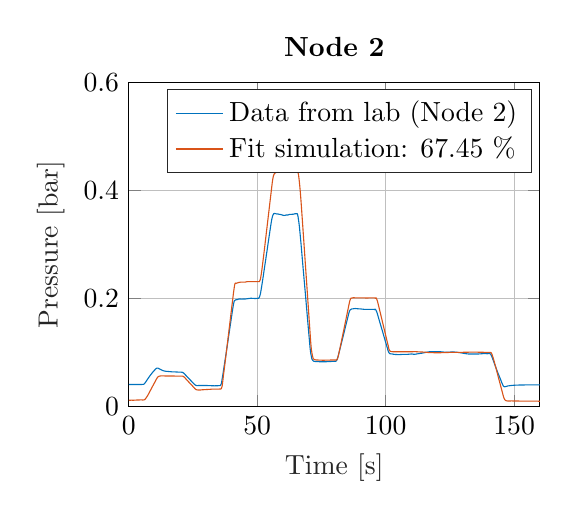
\begin{tikzpicture}

\begin{axis}[%
width=2.0556in,
height=1.62135in,
at={(0.766in,0.486in)},
scale only axis,
xmin=0,
xmax=160,
xlabel style={font=\color{white!15!black}},
xlabel={Time [s]},
ymin=0,
ymax=0.6,
ylabel style={font=\color{white!15!black}},
ylabel={Pressure [bar]},
axis background/.style={fill=white},
title style={font=\bfseries},
title={Node 2},
xmajorgrids,
ymajorgrids,
legend style={legend cell align=left, align=left, draw=white!15!black}
]
\addplot [color=mycolor1]
  table[row sep=crcr]{%
0.0500000000000114	0.0411290322580555\\
5.65000000000001	0.0412878787878697\\
5.84999999999999	0.0417094330400687\\
6.09999999999999	0.0426502932551216\\
6.40000000000001	0.0443242913000859\\
6.65000000000001	0.046010508308882\\
7.90000000000001	0.0548753665689219\\
8.59999999999999	0.0594330400782042\\
9.25	0.0633308895405662\\
9.69999999999999	0.0658235581622648\\
10.6	0.0703995601172949\\
10.8	0.0710471652003832\\
11	0.0714565004887504\\
11.15	0.0715237047898256\\
11.45	0.0712548875855248\\
11.85	0.0703384652981356\\
12.25	0.0693120723362597\\
12.65	0.0683162267839634\\
13.25	0.0669904692082071\\
13.9	0.0661107038123134\\
14.35	0.0657013685239463\\
16.95	0.0645772238514155\\
18.2	0.0644244868035173\\
19.7	0.064027370478982\\
20.3	0.0640945747800572\\
20.8	0.0637768817204289\\
21.05	0.0633247800586503\\
21.3	0.0625427663734115\\
21.65	0.0610703812316729\\
22.5	0.0567509775171118\\
23.15	0.0535801564027452\\
23.85	0.0500794232649184\\
24.75	0.0455156402736918\\
25.35	0.0424364613880641\\
25.75	0.0407380254154361\\
26.05	0.0398338220918788\\
26.3	0.0394061583577638\\
26.65	0.0391556695992108\\
27.55	0.0393206256109409\\
28.95	0.0393328445747727\\
30.45	0.039308406647109\\
30.8	0.0391984359726223\\
33.35	0.0387402248289277\\
35.55	0.0390884652981356\\
35.7	0.0395283479960824\\
35.85	0.0405608504398742\\
36	0.0421554252199314\\
36.05	0.0428274682306835\\
36.1	0.0438172043010638\\
36.2	0.0466092375366713\\
36.3	0.0496395405669716\\
36.55	0.0567509775171118\\
36.65	0.0597629521016643\\
36.8	0.0645039100684244\\
37.05	0.0724828934506263\\
37.35	0.0816898826979582\\
37.65	0.090780791788859\\
37.9	0.0984848484848442\\
38.15	0.106537145650037\\
38.35	0.112994868035202\\
38.7	0.124230205278593\\
38.95	0.132361925708693\\
39.25	0.141843841642242\\
39.45	0.148289345063546\\
40.25	0.173765884652994\\
40.65	0.186070381231673\\
40.75	0.188728005865102\\
40.9	0.192289833822088\\
41.05	0.195326246334304\\
41.1	0.195912756598233\\
41.2	0.1963220918866\\
41.35	0.196768084066463\\
41.55	0.197525659824038\\
41.7	0.19783724340175\\
42.3	0.198350439882688\\
42.85	0.199334066471152\\
42.95	0.199425708699891\\
43.4	0.199315738025405\\
44.15	0.199260752688161\\
44.3	0.199309628543489\\
45.35	0.199450146627555\\
45.65	0.199511241446714\\
45.8	0.19968230694036\\
47.5	0.20076368523948\\
48.05	0.200635386119245\\
48.35	0.200507086999011\\
49.1	0.200354349951112\\
49.45	0.200262707722374\\
49.7	0.200415444770272\\
49.8	0.200415444770272\\
50	0.200464320625599\\
50.55	0.200818670576723\\
50.75	0.201845063538599\\
50.95	0.203910068426183\\
51.05	0.205290811339182\\
51.15	0.207093108504381\\
51.35	0.211375855327475\\
51.45	0.214155669599222\\
51.75	0.222776148582597\\
52.4	0.242876344086028\\
52.6	0.249444037145651\\
52.8	0.255797898338216\\
52.95	0.260716031280538\\
53.1	0.265371456500475\\
53.2	0.268585043988253\\
53.35	0.273191593352891\\
53.4	0.274804496578696\\
53.55	0.280028103616814\\
53.8	0.287616080156397\\
53.95	0.292534213098719\\
54.1	0.297666177908098\\
54.25	0.302413245356803\\
54.35	0.305816226783975\\
54.7	0.31688049853372\\
54.95	0.324932795698913\\
55.15	0.331188905180824\\
55.25	0.334310850439891\\
55.45	0.340499755620726\\
55.55	0.343401759530792\\
55.75	0.34846041055718\\
55.9	0.351270772238507\\
56	0.352950879765388\\
56.15	0.354820381231661\\
56.4	0.357032013685227\\
56.55	0.357386363636351\\
56.65	0.357349706744856\\
56.75	0.357655180840652\\
57	0.357410801564015\\
57.2	0.357380254154435\\
57.5	0.356744868035179\\
57.7	0.356836510263918\\
57.85	0.356836510263918\\
57.95	0.356720430107515\\
58.05	0.356738758553263\\
58.45	0.356213343108493\\
58.5	0.356011730205267\\
58.95	0.355999511241436\\
59.05	0.355645161290312\\
59.75	0.354875366568905\\
59.95	0.354356060606051\\
60.05	0.354453812316706\\
60.25	0.354148338220909\\
60.4	0.353965053763432\\
60.6	0.354209433040069\\
60.8	0.354136119257078\\
61.25	0.354814271749774\\
61.5	0.35462487781038\\
61.65	0.354924242424261\\
61.75	0.354728739002951\\
61.95	0.35498533724342\\
62.05	0.355009775171084\\
62.1	0.354960899315756\\
62.35	0.355559628543517\\
62.7	0.355920087976557\\
62.95	0.356011730205296\\
63.3	0.356048387096791\\
63.7	0.356146138807446\\
63.75	0.356280547409597\\
63.95	0.356225562072353\\
64.4	0.356683773216048\\
64.5	0.356799853372451\\
64.65	0.357196969696986\\
64.75	0.357196969696986\\
64.85	0.357435239491707\\
64.95	0.357465786901287\\
65.05	0.357203079178902\\
65.2	0.35719086021507\\
65.35	0.357410801564043\\
65.55	0.357215298142734\\
65.7	0.355938416422305\\
65.75	0.355156402737066\\
65.85	0.352963098729248\\
65.9	0.351631231671576\\
66	0.348454301075293\\
66.1	0.345197947214075\\
66.2	0.342106549364615\\
66.25	0.34038978494624\\
66.35	0.336412512218971\\
66.45	0.331970918866091\\
66.6	0.324822825024455\\
66.75	0.317546432062585\\
67.05	0.301942815249276\\
67.15	0.296480938416437\\
67.3	0.288184261974607\\
67.5	0.277144428152496\\
67.65	0.268811094819171\\
67.75	0.263257575757592\\
67.85	0.257710166177901\\
68	0.249590664711633\\
68.1	0.244354838709683\\
68.3	0.233522727272742\\
68.65	0.21469941348974\\
68.9	0.200995845552313\\
69.6	0.162115102639291\\
69.7	0.156592130987292\\
70.1	0.13487292277614\\
70.25	0.126887829912022\\
70.35	0.121419843597266\\
70.45	0.115976295210174\\
70.5	0.113214809384147\\
70.55	0.110722140762448\\
70.7	0.104062805474086\\
70.75	0.102132209188653\\
70.85	0.0989736070381184\\
70.95	0.0962671065493623\\
71.15	0.0916666666666686\\
71.25	0.089510019550346\\
71.3	0.0887096774193594\\
71.4	0.087561094819165\\
71.55	0.0863453079178953\\
71.75	0.0851111925708778\\
71.9	0.0845246823069488\\
72.05	0.0842069892473205\\
72.4	0.0838648582600285\\
74.5	0.0832416911046039\\
75.7	0.083229472140772\\
76.65	0.0832600195503517\\
78.3	0.0837121212121303\\
79.05	0.0838770772238604\\
80.6	0.0842069892473205\\
80.75	0.084671309872931\\
80.9	0.0855266373411609\\
81.05	0.0868035190615899\\
81.15	0.0879032258064569\\
81.5	0.0936217008797655\\
81.7	0.0971285434995082\\
82.4	0.110282258064501\\
82.85	0.118749999999977\\
83.3	0.127437683284455\\
83.8	0.137237292277604\\
84.05	0.141990469208196\\
84.55	0.151686217008773\\
84.65	0.153696236559114\\
84.8	0.156573802541516\\
85.65	0.172770039100669\\
85.75	0.174468475073297\\
85.9	0.176472385141722\\
86	0.17761485826\\
86.15	0.179111681329402\\
86.7	0.180834555229694\\
87.15	0.181231671554229\\
87.3	0.181231671554229\\
87.7	0.181579912023437\\
88.2	0.181769305962831\\
89.65	0.181127810361659\\
89.75	0.181182795698902\\
90.2	0.180993401759508\\
90.6	0.18081011730203\\
90.85	0.180669599217964\\
91.05	0.180602394916889\\
91.2	0.180437438905159\\
91.85	0.180193059628522\\
92.35	0.180290811339177\\
92.55	0.180272482893429\\
92.9	0.180217497556185\\
93.65	0.180089198435951\\
94.95	0.180266373411513\\
95.4	0.180254154447681\\
95.55	0.180193059628522\\
95.7	0.179734848484827\\
95.75	0.179899804496557\\
95.8	0.180321358748756\\
95.85	0.180522971651982\\
95.95	0.18034579667642\\
96.05	0.179936461388053\\
96.2	0.178934506353841\\
96.45	0.176515151515133\\
96.55	0.175262707722368\\
96.75	0.172403470185714\\
96.9	0.169904692082099\\
97.7	0.15673264907133\\
97.95	0.152755376344061\\
98.85	0.138306451612891\\
99.1	0.13412145650048\\
99.4	0.129062805474092\\
100.5	0.11103372434016\\
100.6	0.109567448680338\\
100.7	0.108253910068413\\
100.75	0.107221407624621\\
100.8	0.105975073313772\\
100.85	0.104960899315728\\
100.95	0.103494623655905\\
101.05	0.102260508308888\\
101.25	0.100360459433034\\
101.4	0.0992974095796626\\
101.55	0.0985703812316672\\
101.75	0.0980388563049814\\
101.95	0.0979533235581584\\
102.55	0.0976417399804461\\
103.25	0.0969330400781985\\
103.5	0.0968719452590392\\
103.95	0.0967069892473091\\
105.15	0.0964198435972605\\
106.3	0.0968291788856561\\
108.45	0.0969758064516668\\
110.15	0.0976906158358304\\
110.75	0.0971896383187243\\
111.2	0.0970185728250783\\
111.65	0.0973423753666225\\
113.55	0.0988330889541089\\
113.85	0.0989369501466797\\
116.5	0.101392961876883\\
116.75	0.101557917888613\\
117.5	0.102040566959971\\
121.1	0.101900048875905\\
121.5	0.101722873900343\\
122.7	0.101154692082162\\
123.95	0.101148582600246\\
124.2	0.101148582600246\\
124.65	0.101191348973657\\
126.7	0.101282991202396\\
127.7	0.100885874877861\\
128.35	0.100336021505427\\
128.75	0.10009164222879\\
128.95	0.0999938905181352\\
129.25	0.0997861681329937\\
129.8	0.0993707233627106\\
131	0.0983443304008347\\
131.3	0.098148826979525\\
132.1	0.097727272727326\\
132.4	0.0975317693060163\\
132.65	0.0975745356794278\\
133.05	0.0976539589443348\\
134.4	0.0976600684262507\\
135.4	0.0975745356794278\\
136.45	0.0977394916911578\\
136.8	0.0979349951124675\\
137	0.0979411045943834\\
137.3	0.0980816226784498\\
137.6	0.0981732649071887\\
138.2	0.0983260019550869\\
139.55	0.0981366080156931\\
140.15	0.0984115347019099\\
140.5	0.0983870967742462\\
140.6	0.0981854838710206\\
140.75	0.097641739980503\\
140.95	0.0964076246334855\\
141.15	0.0946603128055301\\
141.35	0.0924731182795995\\
141.65	0.0886730205278923\\
141.95	0.0846652003910435\\
143.05	0.0704484359726507\\
143.6	0.063605816226783\\
144.2	0.0565371456500543\\
144.45	0.0536656891495397\\
144.9	0.0482465786901116\\
145.2	0.0445808895405548\\
145.6	0.0400659824046556\\
145.75	0.0388135386118904\\
145.95	0.0377077223851074\\
146.15	0.0371456500488421\\
146.35	0.0370234604105235\\
146.65	0.0372922776148243\\
147.6	0.0385386119256736\\
149.15	0.0395222385141381\\
151.2	0.0401087487780671\\
155.6	0.0404814271749387\\
160	0.0404386608015272\\
};
\addlegendentry{Data from lab (Node 2)}

\addplot [color=mycolor2]
  table[row sep=crcr]{%
0.0500000000000114	0.011956256109471\\
0.800000000000011	0.0120967741935374\\
1.05000000000001	0.0121639784946126\\
2	0.0120601173020418\\
2.55000000000001	0.0123594819159223\\
2.84999999999999	0.0123350439882586\\
3.09999999999999	0.0124389051808294\\
3.69999999999999	0.0125061094819046\\
4.80000000000001	0.0126710654936346\\
5	0.0126466275659709\\
5.55000000000001	0.0125183284457364\\
6	0.0127016129032143\\
6.19999999999999	0.0131659335288248\\
6.5	0.0145833333333201\\
7	0.0179802052786044\\
7.5	0.0217436461388161\\
7.69999999999999	0.0235581622678467\\
9.55000000000001	0.0401392961876752\\
9.94999999999999	0.0436094819159223\\
10.8	0.0512402248289447\\
11.1	0.0536168132942407\\
11.25	0.0545332355816299\\
11.45	0.0554496578690191\\
11.8	0.0564455034213154\\
12.05	0.0567693059628596\\
12.65	0.0572152981427223\\
13.45	0.057154203323563\\
14.25	0.0569159335288418\\
14.45	0.0568914956011781\\
14.65	0.0568853861192622\\
16.35	0.0569342619745896\\
17	0.0568487292277666\\
17.75	0.0568792766373463\\
18.1	0.0566959921798684\\
20	0.0567631964809436\\
20.55	0.0567204301075321\\
21	0.0566410068426251\\
21.2	0.0562622189638375\\
21.45	0.0554252199413554\\
21.65	0.0545576735092936\\
22	0.0528653470185816\\
22.35	0.0510141739980554\\
22.75	0.0489491691104718\\
23.1	0.0472385141740119\\
23.4	0.0456256109481785\\
24.4	0.0405364125122105\\
24.8	0.0385813782991136\\
25.65	0.0340603616813269\\
26.05	0.0322091886608007\\
26.25	0.031677663734115\\
26.55	0.0312438905180841\\
27.1	0.0309811827956992\\
27.95	0.0310422776148584\\
28.35	0.0313233137829911\\
31.9	0.0323252688172033\\
32.2	0.0324963343108493\\
32.8	0.0326979472140749\\
33.1	0.0326490713587475\\
34.55	0.0326368523949156\\
35.85	0.0328506842619731\\
35.95	0.0332661290322562\\
36.1	0.0342069892473091\\
36.15	0.0347446236559108\\
36.3	0.0371334310850386\\
36.35	0.0381109481915871\\
36.4	0.039558895405662\\
36.55	0.0448619257086875\\
36.6	0.046768084066457\\
36.85	0.0571847507331427\\
37.65	0.087554985337249\\
38.4	0.116495601173028\\
38.85	0.134420821114361\\
39.55	0.162328934506348\\
39.8	0.172275171065507\\
40.4	0.19602272727272\\
40.8	0.211265884652988\\
40.9	0.214937683284461\\
41.1	0.221676441837729\\
41.15	0.223118279569889\\
41.3	0.226649560117295\\
41.35	0.227663734115339\\
41.4	0.228201368523941\\
41.55	0.228824535679365\\
41.6	0.228885630498525\\
41.85	0.228366324535671\\
42.35	0.229319403714555\\
42.75	0.229887585532737\\
43.55	0.230620723362648\\
45.4	0.230730694037135\\
46.05	0.231396627565999\\
46.25	0.23145772238513\\
46.6	0.231561583577729\\
47.1	0.231579912023477\\
47.75	0.231641006842636\\
48.05	0.231653225806468\\
48.45	0.231555474095813\\
49.45	0.231653225806468\\
50.05	0.231500488758542\\
50.45	0.23150048875857\\
50.7	0.231573802541561\\
50.85	0.231702101661796\\
50.9	0.231928152492685\\
51.05	0.23321114369503\\
51.1	0.233858748778118\\
51.3	0.237396138807441\\
51.35	0.238526392961887\\
51.6	0.245692815249271\\
51.8	0.252559872922774\\
52.05	0.261638563049843\\
52.8	0.290689149560109\\
53.1	0.302883675464329\\
53.45	0.31704545454545\\
54.55	0.361528592375379\\
54.9	0.375873655913978\\
55.4	0.395931085043998\\
55.85	0.414002932551313\\
55.9	0.415811339198427\\
56.05	0.420717253176917\\
56.1	0.422134652981413\\
56.3	0.426625122189648\\
56.35	0.427517106549374\\
56.6	0.430467986314767\\
56.9	0.432123655913983\\
57.05	0.432746823069408\\
57.55	0.433773216031284\\
57.8	0.434011485826005\\
58.55	0.434145894428156\\
58.95	0.434133675464324\\
59.2	0.434158113391987\\
59.7	0.433987047898341\\
60.9	0.43428641251225\\
61.2	0.434188660801595\\
61.85	0.434054252199445\\
62.15	0.433925953079211\\
64.55	0.434090909090941\\
64.85	0.434231427175007\\
65.75	0.433877077223883\\
65.85	0.433565493646171\\
65.9	0.432942326490746\\
66.05	0.430321358748813\\
66.1	0.428897849462402\\
66.35	0.418908846529831\\
66.55	0.409762952101687\\
66.75	0.399499022482928\\
66.8	0.396627565982413\\
67.05	0.380828445747824\\
67.25	0.367656402737055\\
67.5	0.350635386119279\\
68.1	0.309347507331381\\
70.7	0.128427419354836\\
70.85	0.118334555229723\\
70.9	0.11547531769304\\
71.05	0.107740713587475\\
71.1	0.105687927663723\\
71.3	0.0996334310850386\\
71.4	0.0970369012707692\\
71.55	0.0935300586510266\\
71.75	0.089931573802545\\
71.8	0.0893450635386159\\
72	0.088147605083094\\
72.3	0.0873228250244438\\
72.55	0.0869562561094881\\
73.1	0.0865713587487846\\
73.65	0.086455278592382\\
74	0.0863758553274749\\
74.8	0.0862414467253245\\
75	0.0861498044965856\\
76.1	0.0861253665688935\\
76.5	0.0861742424242493\\
76.9	0.0862353372433802\\
77.45	0.0862597751710723\\
77.8	0.0862353372434086\\
78.05	0.0862475562072405\\
78.5	0.0864674975562139\\
78.8	0.0865469208211209\\
80.7	0.0864797165200457\\
80.85	0.0865652492668687\\
81.05	0.0873350439882756\\
81.15	0.0881598240469259\\
81.3	0.0897360703812353\\
81.5	0.0927724828934515\\
81.6	0.0948435972629511\\
81.95	0.102547653958936\\
82.3	0.110111192570855\\
83.5	0.137524437927681\\
83.8	0.144354838709688\\
85.8	0.190915200391032\\
85.95	0.193976050830912\\
86.1	0.196786412512239\\
86.3	0.199382942326508\\
86.5	0.200830889540583\\
86.6	0.201020283479977\\
86.95	0.20130131964811\\
87.3	0.201637341153514\\
87.75	0.201667888563094\\
88.05	0.201557917888607\\
89.65	0.201521260997112\\
90.05	0.201454056696036\\
92.75	0.201289100684306\\
94.55	0.201454056696036\\
94.8	0.201454056696036\\
95.1	0.201405180840709\\
95.75	0.201325757575802\\
95.85	0.201228005865119\\
96.05	0.200647605083105\\
96.25	0.201454056696008\\
96.3	0.201362414467269\\
96.5	0.199657869012725\\
96.8	0.195204056696014\\
96.95	0.192625855327492\\
97.55	0.180962854349985\\
99.65	0.139259530791833\\
99.85	0.135294477028395\\
100	0.132306940371507\\
100.85	0.115408113392022\\
101	0.113013196480978\\
101.05	0.112017350928681\\
101.25	0.107209188660846\\
101.3	0.106329423264953\\
101.5	0.104062805474143\\
101.8	0.102669843597312\\
102	0.102254398827029\\
102.3	0.10196725317698\\
103	0.101814516129082\\
103.5	0.101722873900343\\
105.2	0.101765640273754\\
107	0.101686217008847\\
107.15	0.101759530791838\\
107.85	0.10183284457483\\
108.2	0.101814516129082\\
110.2	0.101728983382259\\
110.8	0.101930596285484\\
111.35	0.101979472140812\\
111.95	0.101857282502493\\
112.25	0.101710654936511\\
112.6	0.101655669599268\\
113.45	0.101399071358799\\
115.2	0.101069159335339\\
115.4	0.100867546432113\\
115.65	0.100745356793794\\
117.1	0.100183284457529\\
117.6	0.100140518084118\\
118.05	0.10012218963837\\
118.35	0.100073313783042\\
118.6	0.100048875855379\\
118.95	0.0999694525904715\\
121.2	0.0998350439883211\\
121.7	0.100103861192622\\
122.35	0.100103861192622\\
122.65	0.100152737047949\\
123.1	0.100238269794772\\
123.35	0.100299364613932\\
123.55	0.100360459433091\\
124.25	0.100433773216082\\
125.2	0.100623167155476\\
126.1	0.100775904203374\\
126.3	0.100702590420383\\
127.05	0.100592619745896\\
127.75	0.100598729227812\\
128.65	0.100568181818232\\
128.85	0.100568181818232\\
129.1	0.100543743890569\\
129.45	0.100525415444821\\
130.2	0.100757575757626\\
130.55	0.100861436950197\\
131.1	0.100873655914029\\
132	0.100928641251272\\
134.15	0.101093597263002\\
134.8	0.101087487781086\\
136.1	0.100928641251272\\
136.55	0.10078201368529\\
136.85	0.100898093841693\\
137.45	0.100891984359777\\
137.7	0.100824780058701\\
138	0.100769794721458\\
138.45	0.100708699902299\\
139.95	0.100727028348047\\
140.6	0.100568181818232\\
140.8	0.100470430107578\\
141	0.100085532746874\\
141.2	0.09874144672537\\
141.45	0.096114369501521\\
141.65	0.0933162267839975\\
142	0.0877199413490075\\
142.15	0.0852333822092248\\
142.45	0.0800586510264338\\
142.8	0.0739186217008978\\
143.5	0.0612658846529825\\
143.85	0.0547226295210237\\
145.05	0.0331744868035173\\
145.5	0.025109970674464\\
145.75	0.0206072825024251\\
146	0.0165933528836604\\
146.2	0.0143450635385989\\
146.45	0.0125366568914842\\
146.65	0.0116752199413384\\
147.05	0.0109237536656792\\
147.3	0.0107832355816129\\
147.7	0.0105816226783872\\
148.1	0.0106427174975465\\
148.9	0.0107771260996969\\
150.95	0.0106121700879669\\
151.55	0.0106304985337147\\
152	0.0105266373411439\\
152.6	0.0104655425219846\\
152.9	0.0104716520039005\\
154.35	0.0104594330400687\\
159.15	0.0103066959921705\\
159.7	0.0102333822091794\\
159.95	0.0102761485825908\\
160	0.010263929618759\\
};
\addlegendentry{Fit simulation: 67.45 \%}

\end{axis}
\end{tikzpicture}%
    \caption{Estimation comparison for node 2.}
  \end{minipage}
  \hfill
  \begin{minipage}[b]{0.45\textwidth}
    % This file was created by matlab2tikz.
%
%The latest updates can be retrieved from
%  http://www.mathworks.com/matlabcentral/fileexchange/22022-matlab2tikz-matlab2tikz
%where you can also make suggestions and rate matlab2tikz.
%
\definecolor{mycolor1}{rgb}{0.00000,0.44700,0.74100}%
\definecolor{mycolor2}{rgb}{0.85000,0.32500,0.09800}%
%
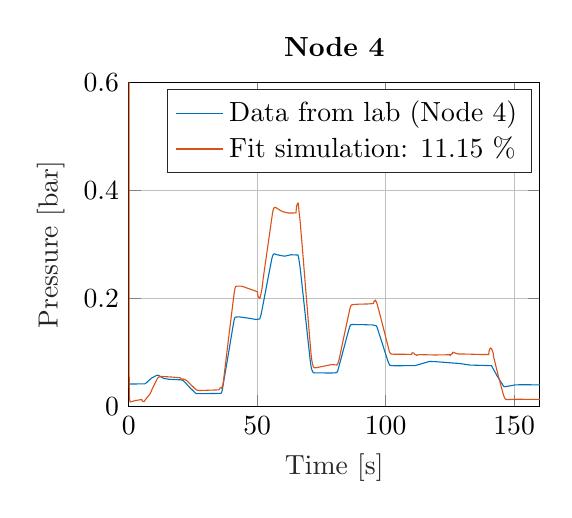
\begin{tikzpicture}

\begin{axis}[%
width=2.0556in,
height=1.62135in,
at={(0.766in,0.486in)},
scale only axis,
xmin=0,
xmax=160,
xlabel style={font=\color{white!15!black}},
xlabel={Time [s]},
ymin=0,
ymax=0.6,
ylabel style={font=\color{white!15!black}},
ylabel={Pressure [bar]},
axis background/.style={fill=white},
title style={font=\bfseries},
title={Node 4},
xmajorgrids,
ymajorgrids,
legend style={legend cell align=left, align=left, draw=white!15!black}
]
\addplot [color=mycolor1]
  table[row sep=crcr]{%
0.0500000000000114	0.0420454545454447\\
6.30000000000001	0.0423326001954933\\
7.05000000000001	0.0451185239491565\\
8.94999999999999	0.0532807917888647\\
10.85	0.0579545454545496\\
11.5	0.0583088954056734\\
12.4	0.0557612414467314\\
13.65	0.0524132453568029\\
15.65	0.0508553274682413\\
20	0.0498533724340291\\
21.1	0.0488636363636488\\
21.85	0.0453812316715414\\
24.15	0.0335838220918845\\
26.2	0.0243890518084129\\
27.2	0.024382942326497\\
30.1	0.0243340664711695\\
35.9	0.0247372922776208\\
36.15	0.0263990713587532\\
36.4	0.0308651026392965\\
36.7	0.0390334799608922\\
37.3	0.0559567448680411\\
38.25	0.0824474584555333\\
40.55	0.147996089931581\\
41.05	0.160764907135871\\
41.25	0.164161779081127\\
41.5	0.165860215053755\\
42.85	0.16642228739002\\
44	0.165603616813286\\
47.35	0.163453079178879\\
48.6	0.16220674486803\\
49.85	0.161455278592371\\
50.95	0.16250610948191\\
51.25	0.165786901270764\\
51.55	0.171407624633417\\
52.2	0.187096774193549\\
54.4	0.242253176930603\\
55.65	0.272763929618748\\
56	0.279142228739005\\
56.3	0.282044232649071\\
56.65	0.283058406647115\\
57.35	0.281738758553274\\
58.2	0.280791788856305\\
59.7	0.279356060606062\\
60.65	0.278586265884655\\
63.2	0.281256109481916\\
65.85	0.280712365591398\\
66.05	0.277535434995116\\
66.3	0.271065493646148\\
66.65	0.25932917888565\\
67	0.245521749755625\\
67.55	0.221169354838736\\
68.5	0.179313294232657\\
69.35	0.142088220918879\\
70.35	0.0980877321603089\\
70.75	0.0814760508309007\\
70.95	0.0748961388074463\\
71.2	0.06932429130012\\
71.6	0.0646994134897625\\
71.95	0.0629948680352186\\
72.6	0.0626466275660107\\
77.75	0.0625122189638603\\
80.1	0.0625610948191877\\
80.95	0.0633247800586787\\
81.25	0.0654081133920101\\
81.6	0.0706378299120445\\
85.55	0.140774682306954\\
86.05	0.148759775171072\\
86.35	0.151374633431089\\
86.75	0.152119990224833\\
90.95	0.152046676441842\\
92.45	0.15167399804497\\
94.85	0.151441837732165\\
96.45	0.149529569892479\\
96.85	0.144330400782025\\
100.75	0.0863208699902316\\
101.5	0.0771749755620874\\
101.9	0.0764846041055876\\
103.55	0.075763685239508\\
109.45	0.0761485826002115\\
110.85	0.0761119257087159\\
111.6	0.0763257575757734\\
117	0.0838037634408693\\
119.2	0.0834799608993251\\
128.75	0.0800158846529939\\
132.85	0.0771016617790963\\
141.15	0.0760813782991363\\
141.7	0.0715909090909008\\
143.35	0.0571725317692824\\
144.75	0.0464992668621562\\
145.95	0.0376282991202004\\
146.4	0.0370295698924394\\
150.55	0.0404814271749387\\
153.5	0.0407930107526511\\
160	0.0404081133919476\\
};
\addlegendentry{Data from lab (Node 4)}

\addplot [color=mycolor2]
  table[row sep=crcr]{%
0.0500000000000114	2.87707747843922\\
0.0999999999999943	0.263649529930916\\
0.150000000000006	0.091497572129839\\
0.199999999999989	0.0452379667079299\\
0.25	0.0270880262064566\\
0.300000000000011	0.0185412293807019\\
0.349999999999994	0.0140836632764376\\
0.449999999999989	0.0102819838409403\\
0.599999999999994	0.00887711426236137\\
0.949999999999989	0.00930013155607412\\
2.34999999999999	0.0112239631609725\\
5.05000000000001	0.013433653955957\\
5.09999999999999	0.0134424671839497\\
5.19999999999999	0.0111297151408962\\
5.34999999999999	0.0102355679974835\\
6	0.00954448752295889\\
6.19999999999999	0.0112418704499078\\
8.19999999999999	0.023271589523489\\
8.80000000000001	0.0286274967850773\\
9.09999999999999	0.0324096773759379\\
11.15	0.0522211657988692\\
11.7	0.054890622736707\\
12.45	0.0560480615677363\\
13.95	0.0557795314013845\\
17.1	0.0548710256818765\\
20.15	0.0535140742142346\\
20.3	0.0521367798952213\\
21	0.0504251019724791\\
21.15	0.0515529413933393\\
21.55	0.0509708142774059\\
22.15	0.0496145054118244\\
22.65	0.0481604085518086\\
25.75	0.03350308746991\\
26.55	0.0306900021199112\\
27.5	0.0300220042901742\\
35.15	0.0312370872850636\\
35.55	0.0346447653953135\\
36	0.0359709543546671\\
36.2	0.0343526919276087\\
36.4	0.0354150288764004\\
36.6	0.0393870322603789\\
36.9	0.0486491980218489\\
37.7	0.0807418994431259\\
39.35	0.145208979577745\\
40.85	0.203209260863787\\
41.2	0.215072864899298\\
41.4	0.219886719561259\\
41.6	0.222195828975231\\
42.05	0.223177353909193\\
43.95	0.223162435944886\\
49.2	0.214430116231568\\
50.1	0.212652391337087\\
50.2	0.207859035942363\\
50.35	0.204532060803757\\
50.7	0.201436698920077\\
51	0.200449526224219\\
51.2	0.204128613945102\\
51.55	0.210506040430971\\
51.85	0.218167021782193\\
51.95	0.221886148357299\\
52.2	0.232266345540467\\
52.65	0.247871749224061\\
55.95	0.357823426835353\\
56.2	0.363729532658709\\
56.45	0.367254685052302\\
56.75	0.368824316062984\\
57.25	0.368677163402594\\
59.15	0.362884355717227\\
60.45	0.36020757408545\\
62.3	0.35841655841017\\
64.4	0.358611294085165\\
65.1	0.358715339183959\\
65.2	0.365165147155153\\
65.3	0.369306201761333\\
65.45	0.372855816858817\\
65.7	0.375942021659711\\
65.95	0.376911120451553\\
66	0.376632194530913\\
66.1	0.369981507467259\\
66.3	0.360897239604213\\
66.6	0.348484218528966\\
66.85	0.336149664653448\\
66.9	0.333358263791837\\
66.95	0.329269423869931\\
67.5	0.298883501771229\\
68.65	0.2308523030392\\
70.55	0.120333832531969\\
70.95	0.0982216638363695\\
71.15	0.0896887479705697\\
71.4	0.082148559540542\\
71.65	0.0768124553414111\\
71.9	0.073783572971422\\
72.25	0.0722155977798877\\
72.9	0.0721769772812024\\
79	0.0780725836005445\\
80.75	0.0773534274079282\\
81.05	0.0773402569705297\\
81.45	0.0806140649421536\\
81.7	0.0843877941200333\\
82.25	0.0955614297302816\\
83.15	0.116450206885418\\
86.15	0.183015793463539\\
86.45	0.186874462757174\\
86.7	0.18830934851934\\
87.5	0.189206914774161\\
89.75	0.189892827340742\\
92.8	0.190132467817989\\
95.2	0.190973964150743\\
95.3	0.192880996713171\\
95.4	0.194122251654989\\
95.55	0.195643091504195\\
95.7	0.195731384587219\\
95.85	0.196208979409136\\
96	0.195501470136151\\
96.05	0.196451577780408\\
96.45	0.193492297209048\\
96.9	0.1871522734954\\
97	0.18433550528394\\
97.95	0.167531215339494\\
100.1	0.127091141525028\\
101.45	0.102110747073567\\
101.75	0.0992938855214618\\
102.15	0.0976885336776547\\
103.15	0.0971679003995973\\
107	0.0970671298743184\\
109.05	0.0970188203601197\\
110.1	0.0970149416945674\\
110.2	0.0993749442153558\\
110.45	0.099827356300068\\
111	0.099435893707664\\
111.1	0.0977786455460432\\
111.45	0.0967550150519969\\
111.9	0.0960372622790544\\
112	0.0950871411506569\\
112.95	0.0964944054075261\\
119.1	0.0957679417689121\\
122.8	0.0960600547285253\\
125.1	0.0962949444237324\\
125.15	0.0950753944568703\\
126	0.0988538737977933\\
126.05	0.100443555811808\\
126.2	0.100872389476535\\
128	0.0977182521800444\\
132	0.0974101265185539\\
136.5	0.0967629955093514\\
140.1	0.0966572788670419\\
140.2	0.101356910842213\\
140.35	0.104924403215335\\
140.55	0.107283259195469\\
140.85	0.108563394216532\\
141.25	0.107211680299059\\
141.8	0.10009203285955\\
141.9	0.0982443519762342\\
141.95	0.0947577381906228\\
142.1	0.0908425116551541\\
143.65	0.0605115003986896\\
145.75	0.0233570142181918\\
146.2	0.0170353357065665\\
146.6	0.0142565079273993\\
147.15	0.0132486303558892\\
150.4	0.0137732874013636\\
151.65	0.0138461249967463\\
157.75	0.013611905149304\\
159.3	0.0135764475834321\\
160	0.0135845159283861\\
};
\addlegendentry{Fit simulation: 11.15 \%}

\end{axis}
\end{tikzpicture}%
    \caption{Estimation comparison for node 4.}
  \end{minipage}
\end{figure}

\begin{figure}[H]
  \centering
  \begin{minipage}[b]{0.45\textwidth}
    % This file was created by matlab2tikz.
%
%The latest updates can be retrieved from
%  http://www.mathworks.com/matlabcentral/fileexchange/22022-matlab2tikz-matlab2tikz
%where you can also make suggestions and rate matlab2tikz.
%
\definecolor{mycolor1}{rgb}{0.00000,0.44700,0.74100}%
\definecolor{mycolor2}{rgb}{0.85000,0.32500,0.09800}%
%
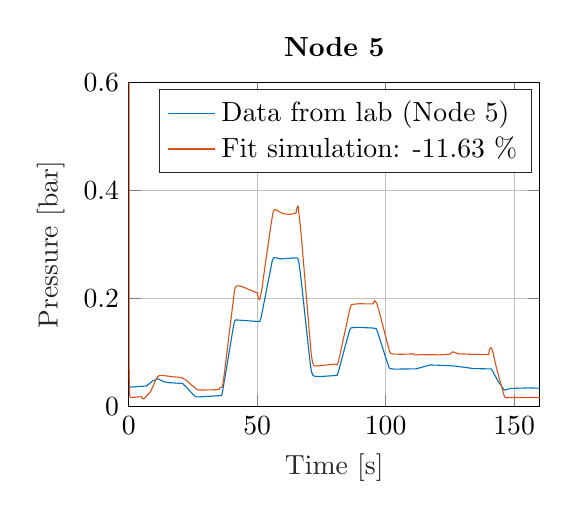
\begin{tikzpicture}

\begin{axis}[%
width=2.0556in,
height=1.62135in,
at={(0.766in,0.486in)},
scale only axis,
xmin=0,
xmax=160,
xlabel style={font=\color{white!15!black}},
xlabel={Time [s]},
ymin=0,
ymax=0.6,
ylabel style={font=\color{white!15!black}},
ylabel={Pressure [bar]},
axis background/.style={fill=white},
title style={font=\bfseries},
title={Node 5},
xmajorgrids,
ymajorgrids,
legend style={legend cell align=left, align=left, draw=white!15!black}
]
\addplot [color=mycolor1]
  table[row sep=crcr]{%
0.0500000000000114	0.0362231182795654\\
6.90000000000001	0.0383980938416357\\
9.5	0.048332111436963\\
11.45	0.0517106549364712\\
12.45	0.0490347018572947\\
13.95	0.045705034213114\\
16.2	0.0444525904203203\\
20.95	0.0430229716519932\\
21.9	0.0389112903225737\\
25.55	0.0203445747800686\\
26.3	0.0182612414467371\\
27.75	0.0183467741935601\\
36.15	0.0207905669599313\\
36.5	0.0273826979472176\\
36.95	0.0402614858259938\\
40.8	0.149822825024444\\
41.15	0.157325268817203\\
41.5	0.160703812316711\\
41.95	0.160551075268813\\
51	0.157594086021504\\
51.35	0.162133431085039\\
51.8	0.171425953079165\\
53.3	0.208088954056706\\
55.85	0.269550342130998\\
56.15	0.273466520039108\\
56.55	0.275898093841647\\
57.1	0.275696480938421\\
58.95	0.273796432062568\\
62.35	0.274450146627572\\
63.5	0.275207722385147\\
64.5	0.275287145650054\\
65.65	0.275549853372439\\
65.95	0.272617302052794\\
66.25	0.26617179863149\\
66.75	0.249236314760509\\
67.3	0.226380742912994\\
70	0.107441348973623\\
70.75	0.0760752688172204\\
71	0.0684567448680582\\
71.25	0.0630620723362938\\
71.7	0.0582783479961222\\
72.2	0.0565860215054101\\
74.3	0.0557612414467599\\
81.1	0.0580461876833169\\
81.45	0.0622922776148869\\
82.1	0.0735276148582784\\
85.1	0.1270711143695\\
86.05	0.142803030303043\\
86.4	0.145423998044976\\
86.85	0.146267106549374\\
89.4	0.146969696969705\\
95.05	0.145680596285445\\
96.3	0.144544232649082\\
96.6	0.141935483870981\\
97.15	0.13389540566962\\
98.2	0.11818792766374\\
99.9	0.0928091397849471\\
101.35	0.0722568426197654\\
101.7	0.07050953079181\\
103.45	0.0696236559140004\\
111.8	0.0700940860215269\\
117.3	0.0773582600195653\\
124.9	0.0760447214076407\\
127	0.0753299120234772\\
134.2	0.0706561583577923\\
141.05	0.0700085532747039\\
141.6	0.0659946236559108\\
143.6	0.0486620234603947\\
146.1	0.0309445259041752\\
146.65	0.0312561094818875\\
148.6	0.0338648582599888\\
155.4	0.034860703812285\\
160	0.0343780547409267\\
};
\addlegendentry{Data from lab (Node 5)}

\addplot [color=mycolor2]
  table[row sep=crcr]{%
0.0500000000000114	3.82183922500244\\
0.0999999999999943	0.276676402994013\\
0.150000000000006	0.104787143988091\\
0.199999999999989	0.058047327977107\\
0.25	0.0392739630695189\\
0.300000000000011	0.0301208295873039\\
0.349999999999994	0.0251240538277386\\
0.449999999999989	0.0203770596337165\\
0.599999999999994	0.0179389039132332\\
0.949999999999989	0.0169619099793294\\
3.05000000000001	0.0179374080923651\\
5.09999999999999	0.0184621098745197\\
5.25	0.0159305204320503\\
5.69999999999999	0.0146649483818919\\
6.15000000000001	0.0152535402844194\\
8.59999999999999	0.0287911715316511\\
8.90000000000001	0.0321648665274097\\
9.55000000000001	0.0385060699697135\\
9.84999999999999	0.042323981862495\\
10.6	0.0503512604374805\\
11.45	0.0566295759956859\\
12.2	0.0581741525921302\\
13.65	0.05770182671111\\
17.15	0.0555570925772599\\
20.25	0.0542007435054188\\
21.15	0.0523737843410004\\
21.65	0.0511605016012311\\
22.6	0.0482093092953733\\
23.9	0.0426300364363215\\
26.75	0.0312140244468253\\
28.4	0.0309302196525607\\
33.95	0.0314541836244757\\
35.2	0.0324100064932509\\
35.6	0.0354006006227507\\
36.1	0.0360059363650294\\
36.3	0.0360742786970434\\
36.5	0.0386718284306653\\
36.8	0.046620210441489\\
37.1	0.0568320834229326\\
39	0.130719208218039\\
41.05	0.210206810432112\\
41.35	0.218632839941733\\
41.55	0.221553614569586\\
42	0.223300955944495\\
43.1	0.223904289606963\\
44.75	0.22104479956576\\
50.1	0.210418045125692\\
50.15	0.207095173779123\\
50.3	0.202936967032429\\
50.55	0.199940496547896\\
51	0.198201901639948\\
51.1	0.201538617251771\\
51.7	0.213532798981959\\
52	0.223029857561016\\
52.4	0.23807647060994\\
55.15	0.329507295992244\\
56.05	0.356813537438256\\
56.3	0.361569506302374\\
56.6	0.364314597187757\\
57.1	0.365073998870457\\
58.7	0.360542193845902\\
60.2	0.3571097048914\\
62.85	0.355915890157974\\
65.15	0.358546682281343\\
65.3	0.364439772109307\\
65.5	0.368299401344984\\
65.85	0.371099590162146\\
66	0.370395279817558\\
66.1	0.364113729070937\\
66.4	0.351094274191809\\
66.7	0.33840533733553\\
67.25	0.311223095666378\\
68	0.2685693271319\\
70.95	0.101652339886613\\
71.2	0.0917362723325823\\
71.5	0.0837014510512688\\
71.75	0.0792922193554091\\
72.05	0.0766957944490798\\
72.65	0.0751795555712818\\
73.95	0.0758188348552551\\
80.2	0.0789109885612049\\
80.85	0.0772817342101177\\
81.15	0.0785132862552018\\
81.6	0.0832891132211842\\
82.1	0.0930976315280816\\
83.2	0.118307581623526\\
86.25	0.184965821104555\\
86.6	0.188238273968608\\
87.4	0.189675461069754\\
89.7	0.190575698096353\\
95.15	0.190293426523255\\
95.65	0.196145195233981\\
96.35	0.192866479447616\\
96.8	0.187435559497487\\
97.8	0.170638090421448\\
100.15	0.126815085328701\\
101.55	0.101855973052466\\
102.05	0.0986494907950259\\
102.95	0.0975011809577779\\
106	0.0970896506505881\\
111	0.0977346187480066\\
111.2	0.096188708580371\\
112.35	0.0957962707120714\\
113.65	0.0963792915596287\\
121.25	0.0960733535974612\\
125.25	0.0974644565331459\\
125.6	0.10039177989492\\
126.2	0.101615502098184\\
128.25	0.0980372625614052\\
133.9	0.0968803205231552\\
140.1	0.0967770681942\\
140.25	0.102504900463828\\
140.45	0.1063939257063\\
140.75	0.108678388725252\\
141	0.109048430497722\\
141.35	0.106768661344688\\
141.9	0.0990312575410144\\
142	0.0953019307828811\\
142.35	0.0878789654078673\\
142.95	0.0755363504925128\\
143.6	0.0632706925558182\\
146.05	0.0212299687878215\\
146.5	0.0175800342550474\\
147.05	0.016427594115811\\
148.2	0.017040462102841\\
150.2	0.017224401374051\\
160	0.0167107640661754\\
};
\addlegendentry{Fit simulation: -11.63 \%}

\end{axis}
\end{tikzpicture}%
    \caption{Estimation comparison for node 5.}
  \end{minipage}
  \hfill
  \begin{minipage}[b]{0.45\textwidth}
    % This file was created by matlab2tikz.
%
%The latest updates can be retrieved from
%  http://www.mathworks.com/matlabcentral/fileexchange/22022-matlab2tikz-matlab2tikz
%where you can also make suggestions and rate matlab2tikz.
%
\definecolor{mycolor1}{rgb}{0.00000,0.44700,0.74100}%
\definecolor{mycolor2}{rgb}{0.85000,0.32500,0.09800}%
%
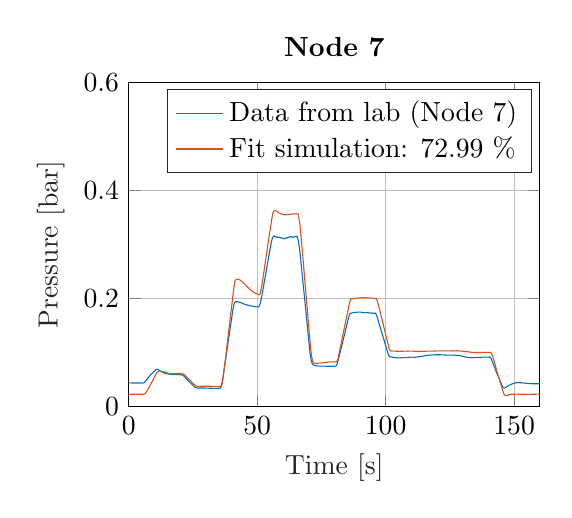
\begin{tikzpicture}

\begin{axis}[%
width=2.0556in,
height=1.62135in,
at={(0.766in,0.486in)},
scale only axis,
xmin=0,
xmax=160,
xlabel style={font=\color{white!15!black}},
xlabel={Time [s]},
ymin=0,
ymax=0.6,
ylabel style={font=\color{white!15!black}},
ylabel={Pressure [bar]},
axis background/.style={fill=white},
title style={font=\bfseries},
title={Node 7},
xmajorgrids,
ymajorgrids,
legend style={legend cell align=left, align=left, draw=white!15!black}
]
\addplot [color=mycolor1]
  table[row sep=crcr]{%
0.0500000000000114	0.0440493646138691\\
0.75	0.0440799120234487\\
2.65000000000001	0.0439821603127939\\
3.19999999999999	0.043969941348962\\
5.09999999999999	0.0438294232648957\\
5.44999999999999	0.0438294232648957\\
5.75	0.0440860215053647\\
5.94999999999999	0.0445075757575637\\
6.15000000000001	0.0452407135874751\\
6.40000000000001	0.0464687194525766\\
6.69999999999999	0.0482893450635515\\
8	0.0562500000000057\\
8.69999999999999	0.0600562072336288\\
9.30000000000001	0.0629337732160309\\
10.55	0.0683101173020475\\
10.8	0.0690676930596226\\
11	0.0693609481915871\\
11.15	0.0693242913000915\\
11.35	0.0690432551319589\\
11.6	0.0683467741935431\\
12.2	0.0663795210166143\\
12.45	0.0655730694037118\\
13.7	0.0625\\
14.5	0.0613758553274693\\
16.15	0.0599034701857306\\
17.2	0.0596529814271776\\
17.55	0.0596407624633457\\
18.7	0.0596346529814298\\
19.05	0.0594758064516157\\
19.55	0.0594330400782042\\
20.15	0.0592253176930626\\
20.4	0.0591825513196511\\
20.7	0.0589626099706777\\
20.95	0.0584799608993194\\
21.2	0.0577590420332399\\
21.6	0.0561461388074349\\
22.4	0.0522727272727366\\
22.65	0.0510263929618873\\
23.35	0.047489002932565\\
23.95	0.0446297653958823\\
25.55	0.0369501466275608\\
25.8	0.0359665200390964\\
26	0.0354777614858222\\
26.35	0.0349034701857249\\
26.65	0.0347690615835745\\
27.55	0.0347996089931542\\
28.05	0.0347751710654904\\
29.25	0.03464076246334\\
29.7	0.0345674486803489\\
30.1	0.0345185728250215\\
31.05	0.0343719452590392\\
31.7	0.0341947702834773\\
34.05	0.034048142717495\\
34.8	0.0341825513196454\\
35.5	0.0342864125122162\\
35.6	0.0344452590420303\\
35.7	0.0349156891495568\\
35.8	0.0355510752688133\\
35.9	0.0364736070381184\\
36	0.0376405180840607\\
36.05	0.0384775171065428\\
36.15	0.0407074780058565\\
36.45	0.0479411045943436\\
36.55	0.0507636852395024\\
36.65	0.0537573313783071\\
36.9	0.0618096285435001\\
37.15	0.0698069403714499\\
37.4	0.0775537634408749\\
38.1	0.100140518084061\\
38.3	0.106702101661767\\
38.45	0.111644672531781\\
38.7	0.119806940371461\\
38.95	0.127779814271747\\
39.65	0.150336021505382\\
39.85	0.156830400782013\\
40.2	0.168053519061573\\
40.4	0.174535679374401\\
40.6	0.180535190615842\\
40.7	0.18322336265885\\
40.85	0.186986803519062\\
40.95	0.189051808406646\\
41	0.189980449657867\\
41.05	0.19069525904203\\
41.15	0.191623900293251\\
41.45	0.194018817204295\\
41.55	0.194348729227755\\
41.7	0.194397605083083\\
41.9	0.194305962854344\\
42.05	0.194244868035184\\
42.45	0.194379276637335\\
43.1	0.193609481915928\\
43.3	0.19323069403714\\
43.4	0.193035190615831\\
43.7	0.192173753665685\\
43.85	0.192082111436946\\
44.15	0.191544477028344\\
44.4	0.191012952101659\\
44.8	0.190255376344084\\
44.9	0.189962121212119\\
45.15	0.189632209188659\\
45.35	0.188996823069402\\
45.5	0.188966275659823\\
45.65	0.188886852394916\\
45.8	0.188581378299119\\
45.9	0.18835532746823\\
46.25	0.188312561094818\\
46.35	0.18799486803519\\
46.65	0.187518328445748\\
46.85	0.187445014662757\\
47.35	0.186821847507332\\
47.5	0.186687438905182\\
47.95	0.186217008797655\\
48.2	0.186052052785925\\
48.5	0.185410557184753\\
48.75	0.185386119257089\\
48.9	0.185227272727275\\
49.1	0.185184506353863\\
49.25	0.185153958944284\\
49.5	0.185043988269797\\
50.1	0.184671309872925\\
50.5	0.184732404692085\\
50.6	0.184946236559142\\
50.75	0.185807673509288\\
50.85	0.186766862170089\\
51.1	0.189778836754641\\
51.2	0.191275659824043\\
51.25	0.192253176930592\\
51.35	0.19447702834799\\
51.45	0.19665200391006\\
51.7	0.202376588465313\\
51.8	0.204967008797666\\
51.9	0.207759042033246\\
52.1	0.212713831867063\\
52.3	0.218230694037146\\
52.75	0.230577956989237\\
52.95	0.235606060606074\\
53.1	0.239503910068436\\
53.2	0.24200268817205\\
53.45	0.249028592375367\\
53.9	0.261601906158347\\
54.05	0.265554740957981\\
54.25	0.271053274682316\\
54.45	0.276441837732165\\
54.9	0.288892961876826\\
55.05	0.293071847507321\\
55.25	0.298075513196466\\
55.35	0.300635386119268\\
55.6	0.306414956011736\\
55.85	0.310746578690129\\
55.95	0.311980694037146\\
56.05	0.31302541544477\\
56.2	0.314192326490712\\
56.3	0.314516129032256\\
56.4	0.315108748778101\\
56.55	0.315829667644181\\
56.65	0.316165689149557\\
56.7	0.316196236559136\\
56.75	0.316043499511238\\
56.9	0.315224828934504\\
57	0.315212609970672\\
57.05	0.315243157380252\\
57.3	0.314595552297163\\
57.5	0.314070136852393\\
57.6	0.313954056695991\\
57.65	0.313721896383186\\
57.7	0.31365469208211\\
57.8	0.313825757575756\\
57.9	0.313874633431084\\
58.05	0.31352028347996\\
58.2	0.313996823069402\\
58.55	0.313477517106548\\
58.7	0.313288123167155\\
58.9	0.313141495601172\\
59.2	0.312707722385142\\
59.3	0.312866568914956\\
59.95	0.311418621700881\\
60.05	0.311241446725319\\
60.15	0.311394183773217\\
60.45	0.310685483870969\\
60.6	0.311162023460412\\
60.7	0.31167521994135\\
60.9	0.311540811339199\\
61.15	0.31213954056696\\
61.3	0.312640518084066\\
61.5	0.312316715542522\\
61.7	0.312090664711633\\
61.85	0.312805474095796\\
61.95	0.313172043010752\\
62.05	0.313165933528836\\
62.15	0.313367546432062\\
62.25	0.313477517106548\\
62.55	0.314222873900292\\
62.8	0.314516129032256\\
62.9	0.314668866080154\\
62.95	0.31487047898338\\
63.05	0.31470552297165\\
63.25	0.314064027370478\\
63.6	0.314057917888562\\
63.75	0.313673020527858\\
63.95	0.313758553274681\\
64.2	0.31421065493646\\
64.35	0.314155669599216\\
64.5	0.314412267839685\\
64.7	0.315163734115345\\
64.75	0.315304252199411\\
65	0.31473607038123\\
65.15	0.314412267839685\\
65.25	0.314797165200389\\
65.35	0.315298142717495\\
65.4	0.315347018572822\\
65.55	0.314809384164221\\
65.6	0.314235092864124\\
65.7	0.312768817204301\\
65.75	0.31217008797654\\
65.8	0.311418621700881\\
65.9	0.309433040078204\\
66	0.307368035190621\\
66.05	0.306482160312811\\
66.1	0.305419110459439\\
66.15	0.303946725317701\\
66.3	0.298478739002945\\
66.65	0.28513563049853\\
66.7	0.283058406647115\\
66.95	0.271505376344095\\
67.1	0.264705522971639\\
67.2	0.260092864125113\\
67.35	0.252755376344084\\
67.45	0.247702834799611\\
67.6	0.240505865102648\\
68.05	0.219086021505376\\
68.35	0.20532135874879\\
68.95	0.17719330400783\\
69.35	0.157612414467252\\
69.5	0.150421554252205\\
69.7	0.140463098729242\\
69.9	0.131054496578685\\
70	0.126429618768327\\
70.15	0.119556451612908\\
70.4	0.107685728250232\\
70.55	0.100928641251215\\
70.6	0.0989491691104547\\
70.75	0.0937683284457478\\
70.85	0.0908846529814298\\
71	0.0869440371456562\\
71.05	0.0854899804496654\\
71.1	0.0842069892473205\\
71.15	0.0832050342131083\\
71.25	0.0817693059628652\\
71.4	0.0803641251222018\\
71.65	0.0782807917888704\\
71.8	0.0776576246334457\\
72.05	0.0769000488758707\\
72.25	0.0765151515151672\\
72.45	0.0764296187683442\\
72.7	0.0761180351906319\\
72.9	0.0759103128054903\\
73.15	0.0758858748778266\\
73.75	0.0754704301075435\\
73.95	0.075262707722402\\
75.55	0.0751221896383356\\
76.1	0.0750488758553445\\
76.4	0.0750427663734285\\
77	0.0748228250244551\\
77.65	0.0748900293255303\\
77.9	0.0750366568915126\\
78.1	0.0749572336266056\\
78.3	0.0749572336266056\\
78.7	0.074835043988287\\
78.95	0.0750244379276808\\
80.1	0.0749022482893622\\
80.3	0.0748228250244551\\
80.6	0.0752749266862338\\
80.75	0.0759042033235744\\
81	0.0778409090909236\\
81.1	0.0788673020527995\\
81.15	0.0795149071358878\\
81.25	0.0813172043010866\\
81.95	0.0945381231671547\\
82.65	0.107844574780046\\
82.95	0.113489736070392\\
83.6	0.126264662756597\\
83.75	0.129227761485822\\
84.05	0.134793499511233\\
84.25	0.138746334310838\\
84.65	0.146761974584535\\
85.35	0.160752688172039\\
85.6	0.165438660801556\\
85.75	0.167870234604095\\
85.95	0.17047287390028\\
86.1	0.172030791788842\\
86.15	0.172391251221882\\
86.25	0.172672287390014\\
86.65	0.173380987292262\\
87.1	0.173912512218948\\
87.25	0.174040811339182\\
87.45	0.174248533724324\\
87.65	0.174334066471147\\
88.2	0.174725073313766\\
88.45	0.174773949169094\\
88.65	0.174859481915917\\
88.75	0.17474951124143\\
89.25	0.175158846529797\\
89.6	0.175042766373394\\
89.9	0.17521383186704\\
90.2	0.175091642228722\\
90.5	0.174963343108487\\
90.85	0.174608993157364\\
91.2	0.174266862170072\\
91.4	0.174004154447687\\
91.75	0.174236314760492\\
91.9	0.17408968719451\\
92.1	0.17408968719451\\
92.25	0.174211876832828\\
92.65	0.174144672531753\\
92.8	0.17408968719451\\
93.15	0.173949169110443\\
93.65	0.173655913978479\\
93.8	0.173710899315722\\
94.15	0.173497067448665\\
94.4	0.173478739002917\\
94.55	0.173380987292262\\
94.7	0.173216031280532\\
94.9	0.173032746823054\\
95.2	0.173099951124129\\
95.35	0.173112170087961\\
95.55	0.173112170087961\\
95.75	0.172696725317678\\
95.8	0.173148826979457\\
95.85	0.173411534701842\\
95.9	0.173484848484833\\
96	0.173002199413475\\
96.35	0.170570625610935\\
96.45	0.16945259042032\\
96.55	0.168084066471152\\
96.8	0.164235092864118\\
96.95	0.161895161290317\\
97.15	0.158528836754641\\
97.3	0.156017839687195\\
97.85	0.147360703812296\\
98	0.145002443792748\\
98.65	0.135025659824038\\
98.9	0.131042277614853\\
99.15	0.127034457478004\\
99.45	0.121945259042036\\
99.9	0.114870478983363\\
100.1	0.111583577712594\\
100.6	0.103500733137821\\
100.7	0.102352150537627\\
100.75	0.10138685239491\\
100.8	0.100134408602145\\
100.85	0.0990835777126051\\
100.9	0.0981915933528796\\
101	0.0970063538611896\\
101.3	0.0940738025415442\\
101.4	0.0933834310850443\\
101.55	0.0927236070381241\\
101.7	0.0924547898338233\\
102	0.0921309872922791\\
102.35	0.0920271260997083\\
102.75	0.0916849951124163\\
104	0.0907502443792794\\
104.55	0.0905486314760537\\
104.9	0.090438660801567\\
105.2	0.0904569892473148\\
105.55	0.0905486314760537\\
105.7	0.0906341642228767\\
108.3	0.0910862658846554\\
108.5	0.0911045943304032\\
108.65	0.0911351417399828\\
109.1	0.0914650537634429\\
109.3	0.0915139296187704\\
109.6	0.0917827468230712\\
109.8	0.0918316226783986\\
110.15	0.0918682795698942\\
111.3	0.091373411534704\\
111.7	0.0917827468230712\\
112.5	0.0922287390029339\\
112.8	0.0924425708699914\\
113.15	0.092735826001956\\
113.5	0.0928274682306949\\
113.7	0.0929618768328453\\
114.05	0.093157380254155\\
114.25	0.0934384164222877\\
115.6	0.0945320136852388\\
115.8	0.0948252688172033\\
116.3	0.0952590420332342\\
118.45	0.095906647116351\\
118.7	0.0960349462365855\\
119.05	0.0961143695014925\\
120.35	0.0962609970675032\\
120.75	0.0963282013685784\\
122.15	0.0959371945259591\\
122.55	0.0959188660802113\\
122.8	0.0958516617791361\\
122.95	0.0958638807429679\\
124.05	0.095436217008853\\
124.65	0.09551564027376\\
125.4	0.0954606549365167\\
125.95	0.0954545454546007\\
126.55	0.0954850928641804\\
127.3	0.095265151515207\\
127.85	0.0951735092864681\\
128.1	0.094923020527915\\
128.3	0.0949657869013265\\
128.6	0.0946419843597823\\
128.8	0.0945442326491275\\
128.95	0.0945686705767912\\
130.3	0.0928946725318269\\
130.6	0.0925708699902827\\
130.8	0.0923631476051412\\
131	0.0922715053764023\\
131.25	0.0919477028348581\\
131.4	0.0918377321603714\\
131.65	0.0916849951124732\\
132.5	0.0910801564027963\\
133.85	0.0909518572825618\\
134.1	0.0909762952102255\\
134.5	0.090933528836814\\
134.7	0.0909762952102255\\
134.9	0.0908907624634026\\
135.05	0.0908174486804114\\
136.05	0.0913245356794334\\
136.6	0.0912573313783582\\
137.2	0.091532258064575\\
137.55	0.0916911045943891\\
137.85	0.091703323558221\\
138.4	0.0917644183773803\\
138.55	0.091788856305044\\
138.7	0.0918316226784555\\
138.9	0.0917094330401369\\
139.9	0.0919660312806059\\
140.2	0.0920882209189244\\
140.45	0.0919293743891103\\
140.65	0.091446725317752\\
140.85	0.0903958944282124\\
141.1	0.0885569403715181\\
141.25	0.0871212121212466\\
141.45	0.0847812805474462\\
141.7	0.0816654447703229\\
142.25	0.0746151026393136\\
142.85	0.067027126099731\\
143.1	0.0639540566960193\\
143.35	0.0610520527859251\\
143.95	0.0543866080156477\\
144.25	0.051014173998027\\
144.65	0.0466703323558022\\
144.9	0.0437744379276523\\
145.5	0.0373411534701518\\
145.65	0.0361986803518732\\
145.8	0.0353372434017274\\
145.95	0.0347812805473779\\
146.1	0.034518572824993\\
146.3	0.0346590909090594\\
146.5	0.0350989736070062\\
148.2	0.0401576246333946\\
149.4	0.0425158846529428\\
150.6	0.0443059628543097\\
151.15	0.0445808895405264\\
152.1	0.0445503421309468\\
153.05	0.0442937438904778\\
155.2	0.0431207233626196\\
157	0.0426075268816817\\
159.35	0.0424670087976153\\
160	0.0425586510263543\\
};
\addlegendentry{Data from lab (Node 7)}

\addplot [color=mycolor2]
  table[row sep=crcr]{%
0.0500000000000114	0.0229472140762539\\
0.449999999999989	0.0229227761485902\\
1.15000000000001	0.0230388563049928\\
1.44999999999999	0.0230510752688247\\
1.94999999999999	0.0231121700879839\\
2.65000000000001	0.0230755131964884\\
3.84999999999999	0.0232465786901344\\
4.30000000000001	0.0231182795698999\\
6	0.0232404692082184\\
6.19999999999999	0.0237292277614927\\
6.40000000000001	0.0244745845552359\\
6.65000000000001	0.0259164222873949\\
7.05000000000001	0.0288062072336288\\
8.5	0.0409885141739892\\
8.94999999999999	0.0450146627565857\\
9.65000000000001	0.0514540566960022\\
10.7	0.0609359726295224\\
11	0.0632881231671547\\
11.2	0.0645405669599199\\
11.4	0.0654325513196454\\
11.6	0.0659152003910037\\
11.85	0.0661412512218931\\
12.35	0.0659396383186674\\
12.95	0.0655730694037118\\
13.75	0.0646444281524907\\
15.65	0.0617668621700886\\
16.1	0.0613453079178896\\
16.7	0.0609787390029339\\
18.85	0.0611009286412525\\
20.35	0.0610642717497569\\
20.85	0.0610398338220932\\
21.3	0.0603250244379296\\
21.65	0.0592008797653989\\
21.95	0.0579239980449699\\
22.45	0.0555779569892536\\
24.2	0.0471529814271605\\
24.45	0.0460410557184616\\
25.05	0.0433223362658737\\
25.3	0.0421126588465199\\
25.8	0.0397971652003832\\
26.1	0.0387280058650958\\
26.4	0.0381353861192508\\
26.75	0.0377321603127996\\
27	0.0377260508308837\\
27.65	0.0378360215053704\\
27.95	0.0379093352883615\\
30.05	0.0380193059628482\\
35.2	0.037524437927658\\
35.6	0.037530547409574\\
35.8	0.0375672043010695\\
36	0.0379154447702774\\
36.05	0.0382270283479897\\
36.2	0.0396810850439806\\
36.25	0.0404630987292194\\
36.45	0.0448497067448557\\
36.5	0.0462793255131828\\
36.8	0.0566043499511295\\
36.9	0.0599767839687217\\
37.05	0.0655180840664684\\
37.2	0.0711388074291222\\
37.75	0.0927847018572834\\
37.95	0.100775904203317\\
38.2	0.110929863147618\\
38.4	0.118884408602156\\
40.55	0.205431329423249\\
40.7	0.211455278592382\\
40.8	0.215444770283483\\
41	0.222947214076243\\
41.05	0.224621212121207\\
41.2	0.229099462365582\\
41.25	0.230296920821104\\
41.45	0.233657135874864\\
41.5	0.23415811339197\\
41.85	0.235581622678382\\
41.95	0.235978739002917\\
42.25	0.236162023460395\\
42.95	0.23534335288366\\
43.15	0.234738514173984\\
43.45	0.234060361681315\\
43.9	0.232484115347006\\
44.15	0.231341642228728\\
44.45	0.230058651026383\\
44.9	0.228018084066463\\
45.05	0.227339931573795\\
45.2	0.226710654936454\\
45.4	0.225733137829906\\
45.7	0.224272971651999\\
45.9	0.223148826979468\\
46.15	0.221963587487778\\
46.35	0.220894428152491\\
46.55	0.220075757575756\\
46.7	0.219477028347995\\
47.9	0.214467253176934\\
48.1	0.213660801564032\\
48.4	0.212518328445753\\
49.25	0.210166177908093\\
50.65	0.20738025415443\\
50.75	0.207343597262934\\
50.95	0.207642961876815\\
51.1	0.208913734115328\\
51.15	0.209384164222854\\
51.2	0.210117302052765\\
51.4	0.21397849462366\\
51.5	0.21634897360704\\
51.65	0.220155180840663\\
52	0.230333577712599\\
52.1	0.233321114369488\\
52.35	0.241342864125102\\
52.65	0.250702590420332\\
52.85	0.257313049853366\\
53.05	0.263850195503409\\
53.3	0.271975806451621\\
53.8	0.288147605083083\\
54.1	0.298081622678382\\
54.25	0.302840909090918\\
54.55	0.312273949169111\\
54.85	0.32184750733137\\
55.35	0.337255620723369\\
55.65	0.346505376344084\\
55.75	0.34948069403714\\
55.9	0.353580156402728\\
55.95	0.354814271749746\\
56.15	0.358913734115333\\
56.2	0.359707966764404\\
56.4	0.361705767350912\\
56.5	0.362188416422271\\
56.65	0.362732160312788\\
57	0.363123167155408\\
57.1	0.363013196480921\\
57.3	0.362365591397833\\
57.45	0.362182306940355\\
57.55	0.362072336265868\\
57.7	0.361485826001939\\
57.9	0.360697702834784\\
58.3	0.359494134897346\\
58.85	0.35797287390028\\
59.05	0.357380254154435\\
59.3	0.356958699902236\\
59.45	0.356598240469197\\
59.85	0.356048387096791\\
60.3	0.355663489736088\\
60.55	0.355596285435013\\
60.75	0.355419110459451\\
60.85	0.355419110459451\\
61.05	0.355694037145668\\
61.5	0.355541300097769\\
62.3	0.355669599218004\\
62.5	0.355749022482911\\
62.7	0.355852883675482\\
62.9	0.356188905180858\\
63.6	0.356647116324552\\
63.8	0.3566654447703\\
65.25	0.357123655913995\\
65.5	0.356952590420349\\
65.85	0.35699535679376\\
65.9	0.35650048875857\\
66.1	0.353030303030323\\
66.15	0.351838954056717\\
66.45	0.342833577712639\\
66.55	0.33984604105575\\
66.6	0.337933773216065\\
66.8	0.328512952101676\\
66.9	0.32357038123169\\
67.1	0.313330889540595\\
67.35	0.300085532746834\\
67.55	0.28922898338223\\
67.7	0.28105449657869\\
68.55	0.233198924731198\\
69.35	0.188966275659823\\
69.9	0.158577712609969\\
70.05	0.150226050830895\\
70.25	0.139076246334298\\
70.85	0.106286656891484\\
70.9	0.103995601173011\\
71.1	0.0962304496578668\\
71.15	0.0946419843597255\\
71.55	0.0847690615835859\\
71.6	0.0838954056696082\\
71.85	0.0818059628543324\\
72.1	0.0807978983382043\\
72.6	0.0799059139784788\\
73.1	0.0800158846529655\\
74	0.0806390518083901\\
74.8	0.0809567448680184\\
75.3	0.081243890518067\\
75.55	0.0812927663733944\\
76.35	0.081836510263912\\
76.8	0.0821358748777925\\
77.1	0.0823863636363455\\
77.35	0.0824718963831685\\
78	0.0828079178885446\\
78.75	0.0830828445747613\\
79.15	0.0829362170087791\\
79.35	0.0830034213098543\\
79.7	0.0831195014662569\\
79.85	0.0830889540566773\\
80.45	0.0831805962854162\\
80.8	0.0832050342130799\\
80.9	0.0835532746822878\\
81.1	0.0845002443792566\\
81.3	0.086711876832851\\
81.5	0.0898582600195539\\
81.55	0.0908846529814298\\
81.75	0.0958822091886589\\
82.15	0.104997556207223\\
82.55	0.114125122189648\\
82.8	0.119721407624638\\
82.95	0.123161045943306\\
83.35	0.13250244379276\\
85.85	0.190499755620749\\
86.1	0.195326246334332\\
86.25	0.197360703812336\\
86.35	0.198258797653978\\
86.5	0.199340175953097\\
86.55	0.199456256109499\\
86.75	0.199297409579685\\
87.4	0.199835043988287\\
87.95	0.200409335288384\\
88.35	0.200568181818198\\
88.7	0.200867546432079\\
88.95	0.201087487781052\\
89.4	0.201337976539605\\
90.2	0.201380742913017\\
90.5	0.201594574780074\\
91	0.201692326490729\\
91.3	0.201606793743906\\
91.65	0.201643450635402\\
91.85	0.201527370478999\\
92.3	0.201643450635402\\
92.6	0.201588465298158\\
92.85	0.20163123167157\\
93.1	0.201490713587503\\
93.55	0.20130131964811\\
94.1	0.201026392961893\\
94.25	0.201056940371473\\
94.55	0.200934750733154\\
94.95	0.201008064516145\\
95.8	0.200476539589459\\
95.95	0.200109970674504\\
96.05	0.200256598240486\\
96.2	0.20061094819161\\
96.25	0.200568181818198\\
96.45	0.199828934506371\\
96.5	0.199364613880761\\
96.9	0.193578934506377\\
97	0.191813294232674\\
98.2	0.168811094819176\\
98.65	0.160013440860212\\
98.95	0.154313294232651\\
99.3	0.147519550342139\\
99.45	0.144672531769288\\
99.65	0.140719696969683\\
100.6	0.122262952101636\\
101	0.114803274682288\\
101.2	0.110428885630483\\
101.3	0.108706011730192\\
101.45	0.106304985337232\\
101.5	0.105785679374378\\
101.75	0.104423264907126\\
101.95	0.103561827956952\\
102.3	0.103128054740921\\
102.65	0.103048631476014\\
102.95	0.102877565982368\\
103.15	0.102883675464284\\
103.65	0.102871456500452\\
103.95	0.10272482893447\\
104.6	0.102614858260011\\
105	0.102578201368516\\
105.55	0.102584310850432\\
106.9	0.10281036168135\\
107.05	0.10281036168135\\
108.35	0.102840909090958\\
108.55	0.102761485826051\\
109.25	0.10295698924736\\
109.65	0.102865347018621\\
109.9	0.102883675464369\\
110.2	0.102950879765444\\
111.9	0.102474340176002\\
112.55	0.102572091886657\\
112.75	0.102498778103666\\
113.5	0.102633186705816\\
114.2	0.102486559139834\\
114.75	0.102559872922825\\
114.95	0.102529325513245\\
115.3	0.102547653958993\\
115.9	0.102840909090958\\
116.45	0.102908113392033\\
116.8	0.102908113392033\\
117.95	0.102950879765444\\
118.2	0.102816471163294\\
120.4	0.103494623655962\\
121.6	0.103488514174046\\
121.85	0.10351295210171\\
122.2	0.103293010752736\\
122.35	0.103256353861241\\
122.65	0.103329667644232\\
122.85	0.103384652981475\\
123.95	0.103531280547458\\
124.75	0.10328690127082\\
125.45	0.103341886608064\\
125.8	0.103244134897409\\
126.15	0.103231915933577\\
127.6	0.103635141740028\\
127.8	0.103592375366617\\
129.8	0.102963098729276\\
130.05	0.102773704789882\\
130.6	0.102517106549413\\
131	0.102419354838759\\
131.35	0.102156647116374\\
131.7	0.102028347996139\\
132.1	0.101698435972679\\
132.45	0.101356304985387\\
133.35	0.100830889540617\\
133.7	0.100714809384215\\
133.95	0.100641495601224\\
134.35	0.100543743890569\\
134.95	0.100409335288418\\
135.15	0.100415444770334\\
135.45	0.100360459433091\\
135.95	0.100323802541595\\
137.2	0.10045210166183\\
137.35	0.10045210166183\\
137.6	0.100433773216082\\
137.9	0.100568181818232\\
138.3	0.100568181818232\\
138.5	0.100690371456551\\
139.5	0.100580400782064\\
139.75	0.100635386119308\\
140.05	0.100574291300148\\
140.4	0.100445992179914\\
140.8	0.100311583577763\\
140.95	0.0998900293255645\\
141.05	0.0994623655914495\\
141.3	0.0973607038123703\\
141.5	0.0950696480938689\\
141.8	0.0907991202346352\\
142	0.0876955034213438\\
142.4	0.0811094819159734\\
142.65	0.0768817204301229\\
143.35	0.0645833333333599\\
143.65	0.0597751710654961\\
144.05	0.0535373900293337\\
144.4	0.0481304985337374\\
145.85	0.0259469696969461\\
146.05	0.0235642717497342\\
146.3	0.0217680840664514\\
146.5	0.0209066471163055\\
146.7	0.0205828445747613\\
147	0.0206561583577525\\
147.7	0.021548142717478\\
148.1	0.0224951124144468\\
148.4	0.0229105571847299\\
149.05	0.0231060606060396\\
150.05	0.0231304985337033\\
150.65	0.0232771260996856\\
151.65	0.0232587976539378\\
152.2	0.0231977028347785\\
154.15	0.0230571847507122\\
154.5	0.023069403714544\\
155.4	0.0229288856304777\\
155.7	0.0229166666666458\\
156.1	0.0229655425219732\\
160	0.023411534701836\\
};
\addlegendentry{Fit simulation: 72.99 \%}

\end{axis}
\end{tikzpicture}%
    \caption{Estimation comparison for node 7.}
  \end{minipage}
\end{figure}

\begin{figure}[H]
  \centering
  \begin{minipage}[b]{0.45\textwidth}
    % This file was created by matlab2tikz.
%
%The latest updates can be retrieved from
%  http://www.mathworks.com/matlabcentral/fileexchange/22022-matlab2tikz-matlab2tikz
%where you can also make suggestions and rate matlab2tikz.
%
\definecolor{mycolor1}{rgb}{0.00000,0.44700,0.74100}%
\definecolor{mycolor2}{rgb}{0.85000,0.32500,0.09800}%
%
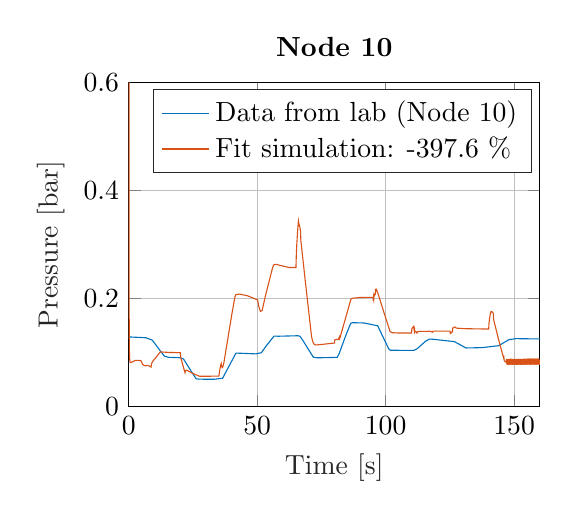
\begin{tikzpicture}

\begin{axis}[%
width=2.0556in,
height=1.62135in,
at={(0.766in,0.486in)},
scale only axis,
xmin=0,
xmax=160,
xlabel style={font=\color{white!15!black}},
xlabel={Time [s]},
ymin=0,
ymax=0.6,
ylabel style={font=\color{white!15!black}},
ylabel={Pressure [bar]},
axis background/.style={fill=white},
title style={font=\bfseries},
title={Node 10},
xmajorgrids,
ymajorgrids,
legend style={legend cell align=left, align=left, draw=white!15!black}
]
\addplot [color=mycolor1]
  table[row sep=crcr]{%
0.0500000000000114	0.129247487781043\\
6.69999999999999	0.127654535679369\\
9.15000000000001	0.123324594330398\\
12	0.105223577712621\\
13.9	0.0935256891495726\\
15.6	0.0914368426197427\\
20.05	0.0907278005865066\\
21.35	0.0882431085044004\\
22.95	0.0759344868035043\\
26.2	0.0518505474095718\\
27.4	0.0510257966764414\\
33.3	0.0508674584555138\\
36.55	0.0527535972629494\\
37.65	0.0627550048875776\\
41.75	0.0993059042033337\\
49.4	0.0978652003909986\\
51.6	0.0999201173020481\\
53.6	0.113062189638327\\
56.55	0.130669051808411\\
58.35	0.130504623655924\\
65.9	0.13140680351907\\
66.7	0.130314965786908\\
67.9	0.121802111436949\\
71.85	0.0916430303030324\\
73.55	0.0905886021505466\\
81.1	0.0913689833822104\\
81.75	0.0965454252199436\\
84.75	0.135220840664715\\
86.4	0.1543380058651\\
87.1	0.155563822091892\\
91.6	0.154992238514183\\
96.9	0.149808836754659\\
101.15	0.107477722385141\\
101.8	0.104587614858275\\
110.95	0.104193509286404\\
112.2	0.107182795698918\\
115.6	0.121521104594336\\
117.05	0.12521508308896\\
118.65	0.124785307917904\\
126.8	0.120445796676449\\
131.25	0.108748778103632\\
137.55	0.109400400782022\\
144	0.113024780058652\\
147.95	0.124133685239485\\
150.7	0.126004164222877\\
160	0.125475210166172\\
};
\addlegendentry{Data from lab (Node 10)}

\addplot [color=mycolor2]
  table[row sep=crcr]{%
0.0500000000000114	6.25508391238557\\
0.0999999999999943	0.527827712429939\\
0.150000000000006	0.225306397698262\\
0.199999999999989	0.144598185290704\\
0.25	0.113053169762708\\
0.300000000000011	0.0984595621127937\\
0.400000000000006	0.0864269265481425\\
0.550000000000011	0.0818627858579362\\
0.900000000000006	0.0818632895341409\\
2.65000000000001	0.0858975226077803\\
3.19999999999999	0.0857482283952038\\
3.65000000000001	0.0858842940624527\\
4.19999999999999	0.0854063924610102\\
4.75	0.085480576517881\\
5.19999999999999	0.0807640402943548\\
5.34999999999999	0.0784092301410908\\
6.19999999999999	0.075732352086618\\
7.44999999999999	0.0764350252007659\\
8.65000000000001	0.0737652271603793\\
8.69999999999999	0.0735132056768464\\
8.84999999999999	0.0791254223369435\\
9.19999999999999	0.0830472032755551\\
12.3	0.101476498013227\\
15.55	0.10053775735696\\
20.1	0.0999912911644287\\
20.2	0.0933468561705979\\
20.4	0.088291022604011\\
21.9	0.0631468328124924\\
22.1	0.0669244564625728\\
22.6	0.0676975768119235\\
24.7	0.0621169863557043\\
27.55	0.0564531592286244\\
35.1	0.0565940863274932\\
35.35	0.0658496216431956\\
35.8	0.0764627181108324\\
36	0.0798406467007737\\
36.15	0.0746797468667353\\
36.4	0.072439167612032\\
36.7	0.0745451522797111\\
37.05	0.0817907359519836\\
40.2	0.172906844730505\\
41.35	0.203663000994794\\
41.7	0.207342191754066\\
43.1	0.208445987200292\\
46.15	0.205465029606955\\
50.2	0.197736868868759\\
50.6	0.185638397187944\\
51.25	0.176510754464516\\
51.95	0.178308796307846\\
53.25	0.206054511627144\\
56.05	0.258319852971312\\
56.55	0.262972463921301\\
57.3	0.263481094406757\\
62.45	0.257574172461034\\
65.1	0.257756041464035\\
65.15	0.26884294653297\\
65.25	0.283322146652182\\
65.4	0.299016390964283\\
65.65	0.319267904767514\\
65.95	0.338901533738749\\
66.05	0.343741272631775\\
66.15	0.340863366344195\\
66.3	0.33739848503069\\
66.5	0.334322131803702\\
66.7	0.330314612257155\\
66.9	0.324562257351005\\
66.95	0.311003136952792\\
67.05	0.305235595370675\\
68.8	0.229153160589306\\
71.15	0.130381879341428\\
71.55	0.121666167613824\\
72	0.116256519147271\\
72.7	0.114308440063212\\
74.95	0.115213556625662\\
80.1	0.117916045483923\\
80.15	0.122197519776449\\
80.3	0.123990233438633\\
81.65	0.125026410312302\\
81.9	0.128166097604861\\
81.95	0.124761962687472\\
82.1	0.125664970765939\\
86.5	0.199267841090347\\
87.15	0.200865283275334\\
89.9	0.20216147644399\\
95.1	0.202410224154278\\
95.2	0.195906413978065\\
95.25	0.199955738489081\\
95.3	0.198807689279249\\
95.35	0.202791141219762\\
95.4	0.201231006147026\\
95.45	0.204982550041564\\
95.5	0.203121077136814\\
95.55	0.206693305765526\\
95.6	0.204622357997692\\
95.65	0.208025602774939\\
95.7	0.205776427408921\\
95.75	0.20904480999846\\
95.8	0.206673880396323\\
95.85	0.209809245198016\\
95.9	0.207300452251616\\
95.95	0.210285592329257\\
96	0.20763427639605\\
96.05	0.217080607010473\\
96.25	0.217896809754819\\
96.5	0.216233120028562\\
97.25	0.206085986594303\\
98.85	0.181750593345555\\
101.7	0.139433864850162\\
102.45	0.137048818006576\\
105	0.136441594610972\\
110.1	0.136521497731877\\
110.15	0.14163946734152\\
110.25	0.1450009117859\\
110.65	0.147318186494147\\
111	0.148916195788757\\
111.05	0.143313728513419\\
111.2	0.138937795211945\\
111.3	0.140784109690088\\
111.35	0.138129939901802\\
111.5	0.139526186773395\\
111.75	0.139307291533441\\
111.95	0.138228974863893\\
112.2	0.136365509671236\\
112.35	0.138488733958297\\
113	0.13941871066919\\
116.5	0.139455571373475\\
116.85	0.139696042643919\\
117.2	0.139927470926096\\
118.3	0.13788375546406\\
118.45	0.14003685077364\\
125.1	0.140052834356084\\
125.15	0.135400017644457\\
125.3	0.135772616250961\\
125.8	0.138468668838897\\
126	0.138362816315208\\
126.05	0.14345435753583\\
126.15	0.145960127945216\\
126.95	0.147699854787703\\
127.5	0.145454287793257\\
130.9	0.14444769776668\\
140.1	0.143741121797007\\
140.2	0.153283761892538\\
140.4	0.162360105498493\\
140.8	0.173045350586619\\
140.9	0.173822134666324\\
140.95	0.176280455327856\\
141.2	0.17595147550449\\
141.45	0.175564091817506\\
141.9	0.172920963001275\\
141.95	0.164443440333173\\
142.1	0.159469046517614\\
144.05	0.122366040426328\\
146	0.0884182478242792\\
146.05	0.0897171232657286\\
146.15	0.0860916433510113\\
146.55	0.083039159149024\\
146.9	0.0823953675891289\\
146.95	0.0840041288771545\\
147.05	0.0822658383881674\\
147.1	0.083887680927262\\
147.2	0.0821840523462072\\
147.25	0.0838054240814756\\
147.35	0.0821599765366727\\
147.4	0.0837929519414331\\
147.5	0.0821283083689934\\
147.55	0.0837470214518987\\
147.65	0.0820931646439931\\
147.7	0.0837229841912404\\
147.8	0.0821012063948672\\
147.85	0.0837571315015566\\
147.95	0.0821787048084559\\
148	0.083859483154697\\
148.1	0.0822595161294259\\
148.15	0.0839417193636791\\
148.25	0.0823485488296001\\
148.3	0.0840316502130918\\
148.4	0.082390446776742\\
148.45	0.0840735091589124\\
148.55	0.0824006777878026\\
148.6	0.084054482987284\\
148.7	0.0823772323423952\\
148.75	0.0840299442859305\\
148.85	0.0823661954266868\\
148.9	0.0840386355902467\\
149	0.0823862615084465\\
149.05	0.0840429677810448\\
149.15	0.0823652940189561\\
149.2	0.0840155718403253\\
149.3	0.082337588225073\\
149.35	0.0839708251447462\\
149.45	0.0822688587380185\\
149.5	0.0838980126673619\\
149.6	0.0822177201287673\\
149.65	0.0838443324634852\\
149.75	0.0821917284435187\\
149.8	0.083847835550614\\
149.9	0.0822027530333003\\
149.95	0.0838472021798964\\
150.05	0.0822068468956161\\
150.1	0.0838571882413248\\
150.2	0.0822127060941682\\
150.25	0.0838586591704313\\
150.35	0.0821931858589835\\
150.4	0.0838333922180823\\
150.5	0.082180397285299\\
150.55	0.0838333218841001\\
150.65	0.0822220175063251\\
150.7	0.0838703797522555\\
150.8	0.0822225892367783\\
150.85	0.0838799412520075\\
150.95	0.0822399146956343\\
151	0.0838944774384629\\
151.1	0.0822573042671308\\
151.15	0.0839177409824003\\
151.25	0.0822643231474842\\
151.3	0.0839213242250594\\
151.4	0.0822951252842472\\
151.45	0.083959229209654\\
151.55	0.082307751975577\\
151.6	0.0839713819733277\\
151.7	0.0823127427352404\\
151.75	0.0839562974293813\\
151.85	0.0822692216442249\\
151.9	0.0839032878363071\\
152	0.0822316565672736\\
152.05	0.0838657839103973\\
152.15	0.0822058355198578\\
152.2	0.0838463641080409\\
152.3	0.0821962570958021\\
152.35	0.0838451295840912\\
152.45	0.0822079311493553\\
152.5	0.0838497016540884\\
152.6	0.0822172756475936\\
152.65	0.0838696989910659\\
152.75	0.0822428636688528\\
152.8	0.0838986591664366\\
152.9	0.0822527607182337\\
152.95	0.0838943176695466\\
153.05	0.0822379089973708\\
153.1	0.0839092346495534\\
153.2	0.0822877674674203\\
153.25	0.0839425661842199\\
153.35	0.0823154365278072\\
153.4	0.0839942899192181\\
153.5	0.0823668632503427\\
153.55	0.0840527745019131\\
153.65	0.0824360175512879\\
153.7	0.0841317932902825\\
153.8	0.0825123254976745\\
153.85	0.0842023389922986\\
153.95	0.0825257887660769\\
154	0.0842043855112138\\
154.1	0.0825264669503838\\
154.15	0.0842056304358039\\
154.25	0.0825397473844305\\
154.3	0.0842300294595475\\
154.4	0.0825739759714565\\
154.45	0.0842620965775041\\
154.55	0.0825891715511773\\
154.6	0.084283185823864\\
154.7	0.0826198933411888\\
154.75	0.0843023467041633\\
154.85	0.0826135516079205\\
154.9	0.0843143512259417\\
155	0.082657599809437\\
155.05	0.0843606482171708\\
155.15	0.0826662484483336\\
155.2	0.0843526615123551\\
155.3	0.0826675307237679\\
155.35	0.0843605877171854\\
155.45	0.0826725570815938\\
155.5	0.0843670907525507\\
155.6	0.0826736321057524\\
155.65	0.0843597582502582\\
155.75	0.0826499761172101\\
155.8	0.0843339945625701\\
155.9	0.0826453341717013\\
155.95	0.0843410620148859\\
156.05	0.0826514032600301\\
156.1	0.0843387215803943\\
156.2	0.0826573865700766\\
156.25	0.0843617576502993\\
156.35	0.0826700024130105\\
156.4	0.0843524690982349\\
156.5	0.0826626601320299\\
156.55	0.0843552476247282\\
156.65	0.0826773653236899\\
156.7	0.0843712172865594\\
156.8	0.082685626361922\\
156.85	0.0843832597623191\\
156.95	0.0826825573658994\\
157	0.0843764826926474\\
157.1	0.0826959940460483\\
157.15	0.0843914291868657\\
157.25	0.0826923396366794\\
157.3	0.0843768932614353\\
157.4	0.0826707361908348\\
157.45	0.0843551749371443\\
157.55	0.0826576733559534\\
157.6	0.0843397903741163\\
157.7	0.0826367084765138\\
157.75	0.0843300092793697\\
157.85	0.082630393199338\\
157.9	0.0843061321044729\\
158	0.0826352181728112\\
158.05	0.0843285012419983\\
158.15	0.0826393456371193\\
158.2	0.084331493637535\\
158.3	0.0826448412013576\\
158.35	0.0843329472144774\\
158.45	0.082648885981996\\
158.5	0.0843364896811636\\
158.6	0.0826434543327537\\
158.65	0.0843277579148491\\
158.75	0.0826339441381094\\
158.8	0.0843270534078897\\
158.9	0.0826421348454573\\
158.95	0.0843274386687938\\
159.05	0.0826454431023365\\
159.1	0.0843515860265427\\
159.2	0.082676402763866\\
159.25	0.0843633599578766\\
159.35	0.0826498121352017\\
159.4	0.0843360485107496\\
159.5	0.0826410917680107\\
159.55	0.0843275117115354\\
159.65	0.0826206480024041\\
159.7	0.0842897760736321\\
159.8	0.0825903977724636\\
159.85	0.084274824785183\\
159.95	0.0825905001343017\\
160	0.0842732918809759\\
};
\addlegendentry{Fit simulation: -397.6 \%}

\end{axis}
\end{tikzpicture}%
    \caption{Estimation comparison for node 10.}
  \end{minipage}
  \hfill
  \begin{minipage}[b]{0.45\textwidth}
   % This file was created by matlab2tikz.
%
%The latest updates can be retrieved from
%  http://www.mathworks.com/matlabcentral/fileexchange/22022-matlab2tikz-matlab2tikz
%where you can also make suggestions and rate matlab2tikz.
%
\definecolor{mycolor1}{rgb}{0.00000,0.44700,0.74100}%
\definecolor{mycolor2}{rgb}{0.85000,0.32500,0.09800}%
%
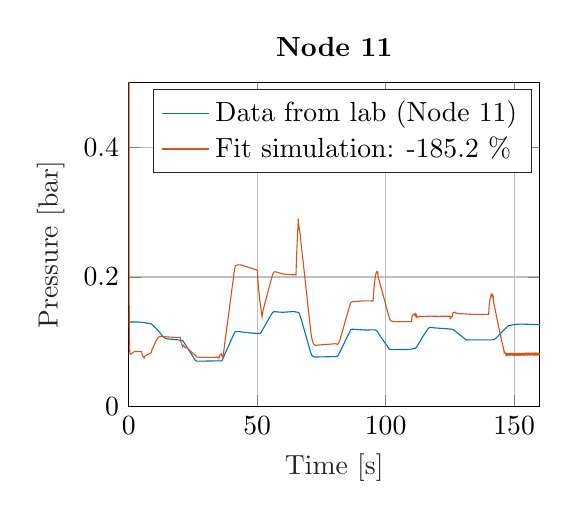
\begin{tikzpicture}

\begin{axis}[%
width=2.0556in,
height=1.62135in,
at={(0.766in,0.486in)},
scale only axis,
xmin=0,
xmax=160,
xlabel style={font=\color{white!15!black}},
xlabel={Time [s]},
ymin=0,
ymax=0.5,
ylabel style={font=\color{white!15!black}},
ylabel={Pressure [bar]},
axis background/.style={fill=white},
title style={font=\bfseries},
title={Node 11},
xmajorgrids,
ymajorgrids,
legend style={legend cell align=left, align=left, draw=white!15!black}
]
\addplot [color=mycolor1]
  table[row sep=crcr]{%
0.0500000000000114	0.130694281524939\\
3.69999999999999	0.130651652003905\\
6.19999999999999	0.129741642228737\\
7.05000000000001	0.128711573802548\\
8.34999999999999	0.128618484848488\\
9.09999999999999	0.126835874877798\\
10	0.123143636363636\\
11.35	0.117936744868047\\
12.25	0.113769491691102\\
13	0.10960571847508\\
14	0.105916959921785\\
15.05	0.104589354838708\\
19	0.103262619745834\\
21.1	0.101674887585546\\
21.75	0.0978756402737133\\
26	0.0709816324535666\\
26.75	0.0702499706744959\\
36.05	0.0708328641251228\\
36.4	0.0720186608015752\\
36.8	0.0753716031280476\\
37.7	0.0836208504398712\\
41.25	0.115023147605086\\
41.6	0.116038426197463\\
43.15	0.115747849462366\\
45.35	0.114654271749743\\
47.45	0.11378167155425\\
48.35	0.113434545454538\\
51.1	0.113014340175965\\
51.6	0.114988347996103\\
52.35	0.120243958944286\\
54.45	0.135279130009792\\
56	0.145293587487799\\
56.6	0.146802150537638\\
57.45	0.146352365591412\\
58.5	0.14594521016619\\
60.1	0.145665073313779\\
64.05	0.146789100684259\\
66.15	0.145436265884655\\
66.5	0.142530498533716\\
67.2	0.134222961876844\\
69.35	0.104163929618778\\
70.4	0.0894837145650058\\
71.05	0.0813319061583684\\
71.45	0.0785679472140828\\
72	0.0770237145650015\\
72.8	0.0766670185728344\\
81.1	0.0774613196481084\\
81.6	0.0799025122189789\\
82.65	0.0883153176930591\\
86.45	0.118985953079175\\
87.15	0.119535786901281\\
92.35	0.118275171065505\\
95.1	0.118541388074277\\
95.9	0.118535298142717\\
96.6	0.117141573802542\\
97.25	0.112934301075285\\
98.4	0.105976119257093\\
101.45	0.0886676637341282\\
102.1	0.0884875757575685\\
103.1	0.0883892668621797\\
105.3	0.0881978690127028\\
107.45	0.0883100977517017\\
109.4	0.0883979667644326\\
111.65	0.0902806256109443\\
112.4	0.0940842228739029\\
114.45	0.1081284750733\\
116.6	0.120942561094807\\
117.35	0.122468523949181\\
119.25	0.12153676441838\\
125.4	0.119798523949157\\
126.35	0.118824134897352\\
131.45	0.102863294232662\\
132.35	0.103089491691122\\
138.55	0.103152130987297\\
141.5	0.103189540566973\\
142.3	0.103776783968726\\
143.35	0.107388113392005\\
144.75	0.113558954056685\\
147.8	0.125048914956011\\
149.95	0.1266984164223\\
152.45	0.127498807429134\\
159.15	0.126689716520048\\
160	0.126654046920834\\
};
\addlegendentry{Data from lab (Node 11)}

\addplot [color=mycolor2]
  table[row sep=crcr]{%
0.0500000000000114	2.00785248408209\\
0.0999999999999943	0.495954452939998\\
0.150000000000006	0.214822120013139\\
0.199999999999989	0.139892764121015\\
0.25	0.110624109735994\\
0.300000000000011	0.0968201191140565\\
0.349999999999994	0.089240649874796\\
0.400000000000006	0.0857984666619416\\
0.449999999999989	0.0835589653930242\\
0.550000000000011	0.081613391808304\\
0.699999999999989	0.0808105199786837\\
1.05000000000001	0.0822181549039271\\
2.40000000000001	0.0852589920745572\\
2.84999999999999	0.0852824383850361\\
3.19999999999999	0.0854674512690963\\
3.65000000000001	0.085227686097852\\
4	0.0851989783129454\\
4.34999999999999	0.0849219552197269\\
4.80000000000001	0.0849531081254042\\
5.09999999999999	0.0848985592749614\\
5.15000000000001	0.0818656255914902\\
5.25	0.0792590091787986\\
6	0.0752076836893139\\
6.09999999999999	0.0774368444951676\\
6.34999999999999	0.0784657035187024\\
8.69999999999999	0.0830443683090323\\
9.09999999999999	0.0883737186031794\\
10.6	0.10100666963524\\
11.35	0.106240358555681\\
11.9	0.108100021973314\\
12.7	0.108624857489389\\
15.3	0.107596274445598\\
18.05	0.106924576822308\\
20.1	0.106916696130043\\
20.15	0.103738303295813\\
20.25	0.101147753296146\\
20.5	0.0982381166617188\\
21	0.0929039508237111\\
21.05	0.094598240930253\\
21.2	0.0950400760627303\\
21.55	0.0933922150539388\\
22	0.0908373487058043\\
22.3	0.0915426700041451\\
22.85	0.0904453332024673\\
24.55	0.0839875357556537\\
26.65	0.0766632873681203\\
27.8	0.0760494148437658\\
35.1	0.076303425806401\\
35.15	0.0751981660429806\\
35.35	0.077753076121553\\
35.65	0.0805668097838463\\
36	0.0818564902548928\\
36.45	0.0770588185064298\\
36.65	0.0780859581606705\\
36.9	0.0810628828230051\\
37	0.0856512467164805\\
37.25	0.0936725446374282\\
41	0.206235546631973\\
41.3	0.213595391139876\\
41.5	0.216663574249566\\
41.7	0.217863760228511\\
42.75	0.218896835578448\\
43.9	0.218466659127301\\
49.05	0.211822861043146\\
50.1	0.210492249806521\\
50.15	0.204443240178932\\
50.25	0.196904143285394\\
50.45	0.186734398310932\\
51.05	0.162031413145229\\
51.4	0.152815184447377\\
51.9	0.139065143099486\\
52.05	0.143490992555087\\
52.35	0.149202585231336\\
53.35	0.164783340210704\\
55.85	0.201857805295475\\
56.2	0.205817797670591\\
56.55	0.207768064526761\\
57.05	0.208254159096924\\
58.2	0.20683785173739\\
61	0.203814499130573\\
64.85	0.20352569066219\\
65.1	0.203546869064439\\
65.2	0.216505323575092\\
65.35	0.233088089602433\\
65.55	0.252348180291307\\
65.8	0.274242879091787\\
66	0.289946264467261\\
66.05	0.285314882487086\\
66.15	0.280800108464859\\
66.3	0.276487073207818\\
66.75	0.264936661974673\\
66.9	0.260109303009102\\
66.95	0.256865933847763\\
67.1	0.251317104061258\\
67.65	0.23183116503526\\
70.65	0.123787524883653\\
71.05	0.110597466904323\\
71.25	0.105787148074796\\
71.55	0.10081509009558\\
71.85	0.0974386981781947\\
72.2	0.0956253600754735\\
72.85	0.0947865458151966\\
74.45	0.0953965018816518\\
80.65	0.0972324937155236\\
81.15	0.0959379135056224\\
81.6	0.097543168382316\\
82.2	0.102614908997538\\
84.55	0.135844321602633\\
86.25	0.158793927092148\\
86.55	0.160893224529246\\
87	0.161694308960932\\
88.6	0.162486260221129\\
92.05	0.163338337501045\\
95.1	0.163083593939774\\
95.3	0.174864465627849\\
95.45	0.182149406640775\\
95.7	0.191747320860401\\
96.1	0.204059551876384\\
96.6	0.208497521669983\\
96.9	0.208390058457951\\
96.95	0.203594255422871\\
97.05	0.200749833362408\\
99.05	0.17171783656886\\
101.5	0.135761793645742\\
101.8	0.133518822899077\\
102.3	0.132057196053893\\
103.3	0.131285814442492\\
109.1	0.131316207076594\\
110.1	0.131336463405205\\
110.15	0.135419357058822\\
110.25	0.138699315564082\\
110.45	0.14083370482328\\
110.85	0.142814491498484\\
111.1	0.142926725097368\\
111.15	0.142212257151755\\
111.25	0.142553701719606\\
111.3	0.141878338166009\\
111.4	0.142342164572057\\
111.45	0.141628303648332\\
111.5	0.142015948752999\\
111.55	0.141456112943644\\
111.6	0.142237085785609\\
111.65	0.141449102840795\\
111.8	0.141662496065948\\
111.85	0.140928014210346\\
111.9	0.141287757054243\\
111.95	0.137635178807102\\
112.05	0.137442312735374\\
112.5	0.13935269639785\\
112.65	0.138756631886622\\
113.3	0.139397573476941\\
113.45	0.139107623982369\\
114.15	0.139134938219769\\
117.5	0.139737987253881\\
117.75	0.139559996469984\\
118.4	0.13960357847057\\
118.65	0.139563669302674\\
119.1	0.139634548526629\\
119.35	0.139494182550976\\
120.1	0.139562084402144\\
120.35	0.139359871749065\\
120.7	0.139295704625482\\
121.85	0.139545720065314\\
122.1	0.139434064211258\\
123.15	0.139659676145925\\
123.55	0.139581315031961\\
123.7	0.139653630916996\\
123.85	0.139489356601928\\
124.1	0.139503012599874\\
124.4	0.139593115931461\\
124.6	0.13943068600625\\
125.1	0.139593109242128\\
125.15	0.136068215062295\\
125.25	0.136199967781408\\
125.55	0.138477899574156\\
125.9	0.139052554288725\\
126	0.138890936099557\\
126.05	0.14283070072716\\
126.15	0.144789037052249\\
126.55	0.145661545621692\\
127	0.145850108881604\\
127.3	0.144421136992321\\
128.05	0.143873830821292\\
132.85	0.142604646193149\\
135.35	0.142201099821335\\
140.1	0.142427021597172\\
140.15	0.147512657037055\\
140.25	0.153781800518857\\
140.4	0.15992452050827\\
140.6	0.165446826546372\\
140.85	0.170343025421772\\
141	0.17204614439413\\
141.1	0.173578565853063\\
141.35	0.173595115835724\\
141.4	0.171687535426202\\
141.45	0.173487815146586\\
141.6	0.172982874192144\\
141.9	0.169534031447739\\
141.95	0.163664337550927\\
142.05	0.160540639562271\\
142.25	0.156495514471857\\
142.5	0.15159738926809\\
142.7	0.148512407989983\\
142.9	0.144117443025948\\
143.2	0.137761116915044\\
144.35	0.116640519328399\\
144.65	0.111257193448211\\
144.9	0.106079934800817\\
145.65	0.0931337369363519\\
145.7	0.0916901560873669\\
145.8	0.0907051451764289\\
146	0.0872852871761438\\
146.05	0.0854227703960078\\
146.1	0.0861682912130277\\
146.5	0.0824671436496942\\
146.75	0.081570225823242\\
146.8	0.0805675385979612\\
146.85	0.0816024694625241\\
147.1	0.0802201851909388\\
147.15	0.0813570984040268\\
147.4	0.0801391909618019\\
147.45	0.0812892223949859\\
147.7	0.0800823668236319\\
147.75	0.08124061006734\\
148	0.0801995946976319\\
148.05	0.0813885100350831\\
148.3	0.0803425390934649\\
148.35	0.0815279774160729\\
148.6	0.0803632609393787\\
148.65	0.081531852590615\\
148.9	0.0803521670203224\\
148.95	0.081534819019339\\
149.2	0.0803303516507867\\
149.25	0.0814964140994334\\
149.5	0.0802298615365373\\
149.55	0.0813795329224547\\
149.8	0.080188737091504\\
149.85	0.0813547553835861\\
150.1	0.0801950865443644\\
150.15	0.0813593834229209\\
150.4	0.080175310201156\\
150.45	0.0813326056395454\\
150.7	0.0802038358965547\\
150.75	0.081366991541671\\
151	0.0802284042288477\\
151.05	0.0814004437438598\\
151.3	0.080253772564248\\
151.35	0.0814322030000199\\
151.6	0.0802925336009537\\
151.65	0.0814649620240289\\
151.9	0.0802354380577697\\
151.95	0.081390731127243\\
152.2	0.080186236957843\\
152.25	0.0813464040962799\\
152.5	0.0801894331940503\\
152.55	0.0813586189009072\\
152.8	0.0802320463354818\\
152.85	0.0814026897717781\\
153.1	0.0802454759246132\\
153.15	0.0814309412143643\\
153.4	0.0803139720020738\\
153.45	0.0815011928910963\\
153.7	0.0804323440281962\\
153.75	0.0816401066469439\\
154	0.0804909902042823\\
154.05	0.0816752757070276\\
154.3	0.0805140056257869\\
154.35	0.0817124188596381\\
154.6	0.0805589149647972\\
154.65	0.0817603557377424\\
154.9	0.0805868052923699\\
154.95	0.0817926755691758\\
155.2	0.0806169997302391\\
155.25	0.0818111300487203\\
155.5	0.0806270060579948\\
155.55	0.0818214220942082\\
155.8	0.0806009105674548\\
155.85	0.0817911847398136\\
156.1	0.0806049732195504\\
156.15	0.0817983344981883\\
156.4	0.0806152848072088\\
156.45	0.0818077944267657\\
156.7	0.0806314530076122\\
156.75	0.0818283667529727\\
157	0.0806389479105292\\
157.05	0.0818395700776477\\
157.3	0.080635978179231\\
157.35	0.0818237925463166\\
157.6	0.0806026824860453\\
157.65	0.0817865618811595\\
157.9	0.0805784158754079\\
157.95	0.0817721967035254\\
158.2	0.0805989337164306\\
158.25	0.0817926474936712\\
158.5	0.0806014097032346\\
158.55	0.0817920580415432\\
158.8	0.0805950016283532\\
158.85	0.0817890766887501\\
159.1	0.0806156692213449\\
159.15	0.0818183250543711\\
159.4	0.0806018856726496\\
159.45	0.0817899643030273\\
159.7	0.0805625651047706\\
159.75	0.0817422094887377\\
160	0.080549161511442\\
};
\addlegendentry{Fit simulation: -185.2 \%}

\end{axis}
\end{tikzpicture}%
    \caption{Estimation comparison for node 11.}
  \end{minipage}
\end{figure}

\begin{figure}[H]
  \centering
  \begin{minipage}[b]{0.45\textwidth}
    % This file was created by matlab2tikz.
%
%The latest updates can be retrieved from
%  http://www.mathworks.com/matlabcentral/fileexchange/22022-matlab2tikz-matlab2tikz
%where you can also make suggestions and rate matlab2tikz.
%
\definecolor{mycolor1}{rgb}{0.00000,0.44700,0.74100}%
\definecolor{mycolor2}{rgb}{0.85000,0.32500,0.09800}%
%
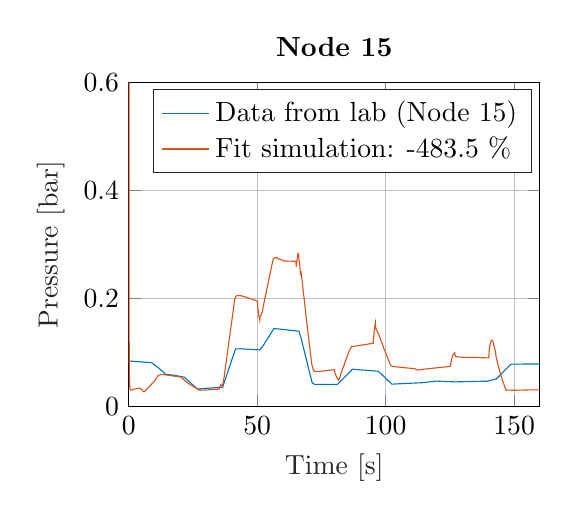
\begin{tikzpicture}

\begin{axis}[%
width=2.0556in,
height=1.62135in,
at={(0.766in,0.486in)},
scale only axis,
xmin=0,
xmax=160,
xlabel style={font=\color{white!15!black}},
xlabel={Time [s]},
ymin=0,
ymax=0.6,
ylabel style={font=\color{white!15!black}},
ylabel={Pressure [bar]},
axis background/.style={fill=white},
title style={font=\bfseries},
title={Node 15},
xmajorgrids,
ymajorgrids,
legend style={legend cell align=left, align=left, draw=white!15!black}
]
\addplot [color=mycolor1]
  table[row sep=crcr]{%
0.0500000000000114	0.0845804496578637\\
8.84999999999999	0.0816346627565849\\
11.95	0.0706084066471249\\
14.45	0.0599231867057597\\
17.5	0.0584589931573873\\
21.6	0.054695415444769\\
26.7	0.0329552297165208\\
36.55	0.0360610948191606\\
38	0.0570348191593268\\
41.6	0.106960078201382\\
43.55	0.107266314760523\\
50.95	0.105078289345073\\
52.05	0.110984652981415\\
56.45	0.144457526881723\\
57.9	0.144153030303016\\
66.3	0.139736959921805\\
67.2	0.124550410557191\\
71.4	0.0442581427174957\\
72.35	0.0414767839687329\\
81.25	0.041502883675463\\
82.6	0.0476215249266829\\
87.1	0.0694365298142827\\
97.15	0.0657007917888563\\
102.4	0.0418195601173181\\
114.2	0.0445356695992132\\
119.75	0.0473901075268941\\
127.05	0.0460729423265036\\
139.45	0.0472448191593458\\
143.05	0.0513711827956911\\
148.75	0.0788533040078221\\
160	0.0792230498533684\\
};
\addlegendentry{Data from lab (Node 15)}

\addplot [color=mycolor2]
  table[row sep=crcr]{%
0.0500000000000114	9.65583948912268\\
0.0999999999999943	0.497739745062006\\
0.150000000000006	0.184910944604326\\
0.199999999999989	0.100894856102343\\
0.25	0.0675119874345\\
0.300000000000011	0.0514005048865442\\
0.400000000000006	0.0378149451047989\\
0.550000000000011	0.0320158005750955\\
0.900000000000006	0.0309547850295075\\
4.05000000000001	0.0347081168541195\\
5.19999999999999	0.03131369765768\\
5.59999999999999	0.0279126597350228\\
6.25	0.0286625960735023\\
10.1	0.0478055629008054\\
11.5	0.058166076660882\\
12.85	0.05992449253921\\
20.25	0.0550638130074503\\
22.3	0.0463594168655845\\
23.95	0.0409047684521795\\
27.6	0.0304011742361183\\
35.2	0.0325981451582322\\
35.8	0.0406308455723376\\
36.15	0.0394962664888681\\
36.5	0.039275679861106\\
36.9	0.0474681490297257\\
37.35	0.0626687703682478\\
41.3	0.199861244146263\\
41.85	0.204988717217162\\
42.6	0.205656638605063\\
42.75	0.205678942620324\\
43.8	0.20535019597213\\
43.9	0.205063124053396\\
48.45	0.198433238458904\\
48.8	0.197269671815775\\
49.15	0.197387898772149\\
49.45	0.196969647185171\\
49.8	0.195839751827464\\
50.1	0.195414831410091\\
50.15	0.188573282989211\\
50.55	0.171215491381361\\
51	0.160297695441926\\
51.1	0.167062320403744\\
51.55	0.169979939941442\\
52.05	0.176844257413478\\
52.75	0.19479048041336\\
56.1	0.270942515744309\\
56.6	0.275498777446188\\
57.7	0.275786704326492\\
58.2	0.273960718716921\\
59.8	0.271306079137105\\
60.1	0.269820759522446\\
65.1	0.269118694005982\\
65.15	0.258851863286338\\
65.9	0.283829563681763\\
66.1	0.28322243802549\\
66.25	0.274701059929271\\
66.6	0.259140844037319\\
66.9	0.243212988592859\\
66.95	0.249920766714098\\
67.05	0.249915050810188\\
67.55	0.230441869609649\\
69.45	0.150068597566985\\
71.2	0.080299700155706\\
71.7	0.0701767986901984\\
72.3	0.0655052323882614\\
73.75	0.065204322876923\\
80.1	0.0685557177792759\\
80.25	0.0629159354867568\\
80.9	0.0546978906295408\\
81.7	0.048948265954607\\
82	0.0510488175005719\\
82.55	0.0607008013298582\\
85.7	0.101935059827525\\
86.7	0.111400935427241\\
88.65	0.112510290171997\\
95.15	0.117516444292789\\
95.35	0.130364842457141\\
95.65	0.143816899160157\\
96	0.154994425756655\\
96.1	0.147287889526979\\
96.35	0.143120060619935\\
97.3	0.133974056277168\\
99.35	0.107364414405254\\
102.05	0.0755245683119483\\
103.7	0.0740518597806101\\
111.4	0.0702982464933655\\
112.35	0.0677805886062117\\
114.15	0.0691097282988835\\
125.2	0.0747240202889827\\
125.6	0.0869039396214077\\
126.15	0.0958307330879791\\
126.9	0.0999827572929632\\
127	0.0951177455772552\\
127.4	0.0925976309382008\\
129.95	0.0915247565368986\\
140.1	0.0904543256477268\\
140.35	0.10615325174021\\
140.65	0.115931595904556\\
141.15	0.123377491709306\\
141.75	0.121316985669637\\
142.15	0.11277863909001\\
142.8	0.100918120047737\\
142.9	0.0944519204483072\\
143.6	0.0799804818790335\\
143.95	0.0738470948553243\\
144.05	0.0712208267260053\\
144.25	0.0684041213786486\\
144.35	0.0658326534488367\\
144.55	0.0631399719402737\\
144.65	0.060563784654903\\
146.75	0.0310799494015725\\
149.6	0.0304512253810856\\
157.2	0.0313209718199801\\
160	0.0312800983863042\\
};
\addlegendentry{Fit simulation: -483.5 \%}

\end{axis}
\end{tikzpicture}%
    \caption{Estimation comparison for node 15.}
  \end{minipage}
  \hfill
  \begin{minipage}[b]{0.45\textwidth}
    % This file was created by matlab2tikz.
%
%The latest updates can be retrieved from
%  http://www.mathworks.com/matlabcentral/fileexchange/22022-matlab2tikz-matlab2tikz
%where you can also make suggestions and rate matlab2tikz.
%
\definecolor{mycolor1}{rgb}{0.00000,0.44700,0.74100}%
\definecolor{mycolor2}{rgb}{0.85000,0.32500,0.09800}%
%
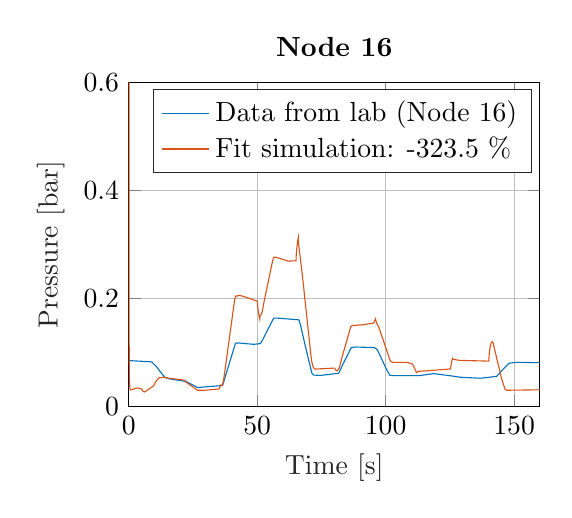
\begin{tikzpicture}

\begin{axis}[%
width=2.0556in,
height=1.62135in,
at={(0.766in,0.486in)},
scale only axis,
xmin=0,
xmax=160,
xlabel style={font=\color{white!15!black}},
xlabel={Time [s]},
ymin=0,
ymax=0.6,
ylabel style={font=\color{white!15!black}},
ylabel={Pressure [bar]},
axis background/.style={fill=white},
title style={font=\bfseries},
title={Node 16},
xmajorgrids,
ymajorgrids,
legend style={legend cell align=left, align=left, draw=white!15!black}
]
\addplot [color=mycolor1]
  table[row sep=crcr]{%
0.0500000000000114	0.0854469599217964\\
9	0.0830370869990134\\
10.85	0.0740700977517008\\
12.5	0.0634353372433907\\
14	0.0549346627566081\\
15.75	0.0516765493646005\\
22.35	0.0467776344086133\\
26.75	0.035629579667642\\
36.55	0.0392696187683157\\
37.55	0.0552174095796545\\
41.55	0.117548729227764\\
42.55	0.118078553274671\\
48.6	0.11549729227761\\
51.3	0.116937126099714\\
52.4	0.126468739002945\\
56.4	0.163987067448687\\
57.5	0.164062756598241\\
60.95	0.162792570869982\\
66.25	0.16080986314762\\
66.9	0.150622277614872\\
68.6	0.114903088954065\\
71.3	0.0618884946236449\\
72	0.0585912316715564\\
74.6	0.0579822385141711\\
81.7	0.0618867546432114\\
83.55	0.0803383773215955\\
86.6	0.109338631476049\\
88.15	0.11052268817204\\
95.7	0.109487399804493\\
96.8	0.105386265884647\\
100.05	0.0719316617790753\\
101.65	0.0582371456500539\\
103	0.0576046627566029\\
113.1	0.0576046627566029\\
118.65	0.0612942913001007\\
125.6	0.0570435190615797\\
129.05	0.0546066764418356\\
136.8	0.0527562072336423\\
143.2	0.0561735288367515\\
145.6	0.0688962658846606\\
148.05	0.0804288563049909\\
150.6	0.0822210361681357\\
160	0.08157202346041\\
};
\addlegendentry{Data from lab (Node 16)}

\addplot [color=mycolor2]
  table[row sep=crcr]{%
0.0500000000000114	7.81748507041465\\
0.0999999999999943	0.465512167911328\\
0.150000000000006	0.173770260157823\\
0.199999999999989	0.0955721356373829\\
0.25	0.0645843143310287\\
0.300000000000011	0.0496835521292951\\
0.349999999999994	0.0417245195478415\\
0.449999999999989	0.0344778646394559\\
0.650000000000006	0.0310002202077158\\
1.25	0.0319119134991013\\
3.40000000000001	0.0349006951418289\\
5.15000000000001	0.0326740938036494\\
5.34999999999999	0.0294165771533983\\
6.09999999999999	0.0271978998252109\\
6.84999999999999	0.0293221199800371\\
9.75	0.0389614788549295\\
10.4	0.0457648055505615\\
11.75	0.0535423492885627\\
13.3	0.0543203295787293\\
21.9	0.0490283622173138\\
22.05	0.0464255770514796\\
26.75	0.0306389341515967\\
29.4	0.030331260571586\\
35.25	0.0330500089906138\\
35.8	0.0401053281937891\\
36.15	0.0402962331764058\\
36.5	0.0403315446254169\\
36.85	0.0475666434650464\\
37.45	0.0667624636546407\\
41.25	0.198761717535461\\
41.7	0.204890675883178\\
42.3	0.204982155107274\\
42.5	0.205840200224344\\
43.35	0.205793077516432\\
44.4	0.204429285497184\\
44.55	0.204288296106029\\
47.2	0.20005598663812\\
47.65	0.199089745962624\\
48.1	0.198649226337636\\
48.55	0.1975432879604\\
49	0.197181478857914\\
49.45	0.196236322493718\\
49.9	0.19589740052777\\
50.1	0.195616968647386\\
50.2	0.185019992324982\\
50.4	0.177669742856125\\
50.7	0.169536132597756\\
51	0.162467159617734\\
51.1	0.167961298719149\\
51.55	0.170779840308569\\
52	0.176436655462823\\
52.6	0.192414876626856\\
56.1	0.272185659261112\\
56.6	0.276797475367005\\
57.45	0.276502030362565\\
62.1	0.269321622212061\\
62.75	0.269719366293458\\
65.1	0.269960377618389\\
65.2	0.280556138050997\\
65.45	0.295066485233036\\
65.75	0.306359062171452\\
66	0.312918448390292\\
66.05	0.304936753688196\\
66.3	0.293672257826842\\
66.7	0.279045972314805\\
68	0.225565158637949\\
68.65	0.195741508493995\\
71	0.0912209107730746\\
71.35	0.0808832201269922\\
71.85	0.0725564327337338\\
72.45	0.0696686458908573\\
74.1	0.0701523371992039\\
80.15	0.0715287667857751\\
80.5	0.068004733381855\\
81.1	0.0663771199500047\\
82	0.0721845637498859\\
83.1	0.0930893991442474\\
86.4	0.147990372379951\\
87	0.150148125050407\\
91.1	0.151700845405713\\
95.35	0.154926460835867\\
96.05	0.162631684645021\\
96.3	0.157776136348303\\
96.65	0.153387060800384\\
96.95	0.150331070370555\\
97.15	0.149605927818925\\
98.25	0.134483879221648\\
101.85	0.0842559727217065\\
102.85	0.0822239600503281\\
108.55	0.0819430542063344\\
110.4	0.0789906153822244\\
111.15	0.0721538482435733\\
112	0.0631748115218329\\
112.65	0.065489998480416\\
116.3	0.0666174458243063\\
125.2	0.0699624094023932\\
125.65	0.082783249631035\\
126	0.0893952408953851\\
126.2	0.0878773069876786\\
128.7	0.0858256327078379\\
140.1	0.0844237223077187\\
140.35	0.0996088814561915\\
140.65	0.110319284099376\\
141.1	0.118854788573913\\
141.5	0.120295388863155\\
141.9	0.117348853531666\\
142.35	0.107149456255598\\
142.9	0.0962827094722627\\
143.45	0.0847355462387611\\
144.35	0.0683420372826617\\
145.05	0.0529834227285448\\
146.45	0.0324518585455564\\
147.2	0.0305368799956796\\
160	0.0312906253486176\\
};
\addlegendentry{Fit simulation: -323.5 \%}

\end{axis}
\end{tikzpicture}%
    \caption{Estimation comparison for node 16.}
  \end{minipage}
\end{figure}

